%versi 3 (22-07-2020)
\chapter{Analisis}
\label{chap:analisis}
Pada bab ini menjelaskan analisis aplikasi WSDC 2017 Bali saat ini dan aplikasi WSDC yang akan dibangun, dan tantangan pada pengembangan sistem usulan. Analisis yang akan dibahas meliputi analisis {\it use case}, analisis kebutuhan sistem, dan analisis pembangunan aplikasi Android WSDC 2017 Bali menggunakan Ionic.

\section{Analisis Sistem Kini dan Sistem Usulan}
\label{sec:analisisSistemKini}
\label{sec:analisisSistemUsulan}

Aplikasi WSDC 2017 Bali digunakan untuk menunjang keberlangsungan acara WSDC 2017 yang diselenggarakan di Bali, Indonesia. Pada halaman utama, pengguna dapat melihat berita-berita terkait acara WSDC 2017 Bali dan tombol {\it read more} yang apabila ditekan akan mengarahkan pengguna untuk melihat berita terkait acara WSDC 2017 Bali dengan format pdf. Aplikasi WSDC 2017 Bali dapat digunakan untuk melihat berita acara, pengumuman, jadwal peserta, lokasi acara, hasil pengundian, info, serta pengumuman pemenang dari acara WSDC 2017 Bali (Gambar~\ref{fig:useCaseDiagram}). 

\begin{figure}[H]
		\centering
	    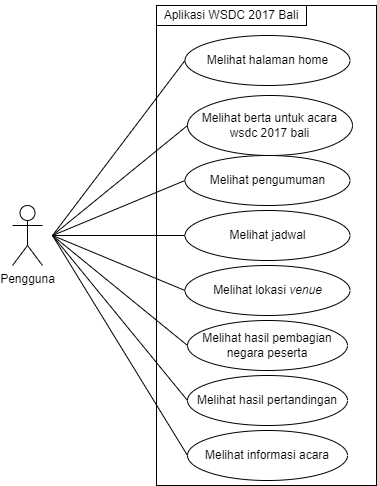
\includegraphics[scale=0.45]{Gambar/useCaseDiagram.png}
	    \caption{{\it Use Case Diagram} Aplikasi WSDC 2017 Bali}
	    \label{fig:useCaseDiagram}
\end{figure}

Terdapat {\it sidemenu} untuk pengguna agar dapat bernavigasi ke dalam menu-menu yang terdapat pada aplikasi WSDC 2017 Bali. Untuk mengakses {\it sidemenu}, pengguna dapat menekan tombol navigasi berada di sebelah kiri atas aplikasi WSDC 2017 Bali. Selain cara tersebut dapat juga dengan cara mengusap layar dari kiri ke kanan. Untuk menutup {\it sidemenu}, pengguna dapat menekan area di luar {\it sidemenu}, atau dengan cara menekan tombol silang di sebelah kiri atas {\it sidemenu}. Terdapat fitur-fitur yang ada pada aplikasi WSDC 2017 Bali yang dapat diakses melalui {\it sidemenu}. Fitur-fitur tersebut adalah sebagai berikut :

\begin{enumerate}
	\item \textit{Home} \\
	Pada halaman ini, pengguna dapat melihat halaman utama aplikasi WSDC 2017 Bali yang berisi berita acara WSDC 2017 Bali, serta pemberitahuan terakhir terkait acara WSDC 2017 Bali. Halaman ini merupakan halaman awal yang ditampilkan saat aplikasi WSDC 2017 Bali pertama kali dibuka (Tabel~\ref{table:skenarioHalamanUtama}). Untuk mengakses halaman ini, dapat melalui \textit{sidemenu}.
		\begin{table}[H]
			\centering
			\caption{Tabel Skenario dari Halaman \textit{Home}}
			\begin{tabular}{|p{0.5cm}|p{7cm}|p{7cm}|}
				\hline
				No & Aksi Aktor                               & Reaksi Sistem                                          \\ \hline
				1  & Pengguna membuka aplikasi WSDC 2017 Bali & Aplikasi WSDC 2017 Bali menampilkan halaman selamat datang. \\ \hline
				2  &                                          & Aplikasi WSDC 2017 Bali menampilkan halaman \textit{Home}           \\ \hline
				3  & Pengguna mengklik {\it card} Announcements & Aplikasi WSDC 2017 Bali menampilkan halaman \textit{Announcement}. \\ \hline
			\end{tabular}
			\label{table:skenarioHalamanUtama}
		\end{table}
	%\end{itemize}
	\item \textit{Newsletter} \\ 
	Pada \textit{bagian newsletter} yang terdapat di \textit{home}, pengguna dapat melihat berita-berita terkait acara WSDC 2017 Bali dengan format pdf. Untuk mengakses halaman ini, dapat melalui \textit{sidemenu} (Tabel~\ref{table:skenarioBerita}).
		\begin{table}[H]
			\centering
			\caption{Tabel Skenario dari \textit{Newsletter}}
			\begin{tabular}{|p{0.5cm}|p{7cm}|p{7cm}|}
				\hline
				No & Aksi Aktor                               & Reaksi Sistem                                          \\ \hline
				1  & Pengguna menekan tombol {\it read more} pada berita di halaman utama aplikasi WSDC 2017 Bali. & Aplikasi WSDC 2017 Bali menampilkan berita pada acara WSDC 2017 Bali \\ \hline
			\end{tabular}
			\label{table:skenarioBerita}
		\end{table}
	%\end{itemize}
	\item \textit{Announcement} \\ 
	Pengguna dapat melihat berbagai pengumuman mengenai keberlangsungan acara WSDC 2017 Bali yang tersusun berdasarkan tanggal dirilisnya pengumuman tersebut. Untuk mengakses halaman ini, dapat melalui \textit{sidemenu} (Tabel~\ref{table:skenarioHalamanPemberitahuan}).
		\begin{table}[H]
			\centering
			\caption{Tabel Skenario dari Halaman \textit{Announcement}}
			\begin{tabular}{|p{0.5cm}|p{7cm}|p{7cm}|}
				\hline
				No & Aksi Aktor                               & Reaksi Sistem                                          \\ \hline
				1  & Pengguna menekan tombol Announcement pada \textit{sidemenu} & Aplikasi WSDC 2017 Bali menampilkan halaman \textit{Announcement}. \\ \hline
			\end{tabular}
			\label{table:skenarioHalamanPemberitahuan}
		\end{table}
	%\end{itemize}
	\item \textit{Schedule} \\ 
	Pada halaman ini, pengguna dapat melihat jadwal acara WSDC 2017 Bali yang ditampilkan berkelompok berdasarkan tanggal dan hari. Jadwal yang ditampilkan berupa waktu mulai dan waktu selesai, lokasi acara, serta nama acara. Untuk mengakses halaman ini, dapat melalui \textit{sidemenu} (Tabel~\ref{table:skenarioHalamanJadwal}).
		\begin{table}[H]
			\centering
			\caption{Tabel Skenario dari Halaman \textit{Schedule}}
			\begin{tabular}{|p{0.5cm}|p{7cm}|p{7cm}|}
				\hline
				No & Aksi Aktor                               & Reaksi Sistem                                          \\ \hline
				1  & Pengguna menekan tombol Schedule pada \textit{sidemenu} & Aplikasi WSDC 2017 Bali menampilkan halaman \textit{Schedule}. \\ \hline
				2  & Pengguna menekan tanggal yang berada di atas halaman jadwal & Aplikasi WSDC 2017 Bali menampilkan jadwal berdasarkan tanggal yang dipilih oleh pengguna dengan detail waktu, lokasi, dan nama kegiatan. \\ \hline
			\end{tabular}
			\label{table:skenarioHalamanJadwal}
		\end{table}
	%\end{itemize}
	\item {\it Venues} \\ 
	Pada halaman ini, pengguna dapat melihat lokasi dari berlangsungnya acara WSDC 2017 Bali. Untuk mengakses halaman ini, dapat melalui sidemenu (Tabel~\ref{table:skenarioHalamanVenues}).
		 \begin{table}[H]
			\centering
			\caption{Tabel Skenario dari Halaman {\it Venues}}
			\begin{tabular}{|p{0.5cm}|p{7cm}|p{7cm}|}
				\hline
				No & Aksi Aktor                               & Reaksi Sistem                                          \\ \hline
				1  & Pengguna menekan tombol \textit{Venues} pada \textit{sidemenu} & Aplikasi WSDC 2017 Bali menampilkan halaman \textit{Venues} yang berisi {\it Ceremony Venues}, {\it Competition Venues}, {\it Delegates Accomodation}, dan {\it Educational Tour}.\\ \hline
				2  & Pengguna menekan kategori {\it venues} yang diinginkan. & Aplikasi WSDC 2017 Bali menampilkan peta, nama lokasi acara dengan disertai penanda yang ada di dalam peta, dan jarak antara lokasi pengguna saat ini dan lokasi acara.\\ \hline
			\end{tabular}
			\label{table:skenarioHalamanVenues}
		\end{table}
	%\end{itemize}

	\item {\it Draw} \\ 
	Pada halaman ini, pengguna dapat melihat pembagian {\it venue} serta pembagian kubu proposisi dan oposisi dari hasil pengundian untuk para negara peserta WSDC 2017 Bali. Untuk mengakses halaman ini, dapat melalui \textit{sidemenu} (Tabel~\ref{table:skenarioHalamanDraw}).
		\begin{table}[H]
			\centering
			\caption{Tabel Skenario dari Halaman {\it Draw}}
			\begin{tabular}{|p{0.5cm}|p{7cm}|p{7cm}|}
				\hline
				No & Aksi Aktor                               & Reaksi Sistem                                          \\ \hline
				1  & Pengguna menekan tombol \textit{Draw} pada \textit{sidemenu} & Aplikasi WSDC 2017 Bali menampilkan halaman \textit{Draw} yang dapat digulir kebawah untuk menampilkan keseluruhan tabel. \\ \hline
			\end{tabular}
			\label{table:skenarioHalamanDraw}
		\end{table}

	\item \textit{Result} \\ 
	Pada halaman ini, pengguna dapat melihat pemenang dari kompetisi WSDC 2017 Bali. Untuk mengakses halaman ini, dapat melalui \textit{sidemenu} (Tabel~\ref{table:skenarioHalamanHasil}).
		\begin{table}[H]
			\centering
			\caption{Tabel Skenario dari Halaman \textit{Result}}
			\begin{tabular}{|p{0.5cm}|p{7cm}|p{7cm}|}
				\hline
				No & Aksi Aktor                               & Reaksi Sistem                                          \\ \hline
				1  & Pengguna menekan tombol \textit{Result} pada \textit{sidemenu} & Aplikasi WSDC 2017 Bali menampilkan halaman \textit{Result} yang berisi pemenang dari babak semifinal, seperempatfinal, dan seperdelapanfinal. \\ \hline
			\end{tabular}
			\label{table:skenarioHalamanHasil}
		\end{table}

	\item Info \\
	Pada halaman ini, pengguna dapat melihat info-info seputar kontak-kontak penting yang dapat dihubungi, kosa kata dalam Bahasa Indonesia sehari-hari, serta {\it credits} kepada pembuat aplikasi WSDC 2017 Bali. Untuk mengakses halaman ini, dapat melalui \textit{sidemenu} (Tabel~\ref{table:skenarioHalamanInfo}).
		\begin{table}[H]
			\centering
			\caption{Tabel Skenario dari Halaman Info}
			\begin{tabular}{|p{0.5cm}|p{7cm}|p{7cm}|}
				\hline
				No & Aksi Aktor                               & Reaksi Sistem                                          \\ \hline
				1  & Pengguna menekan tombol {\it hamburger} di pojok kiri atas atau melakukan \textit{swipe} dari kiri layar ke kanan layar aplikasi WSDC 2017 Bali. & Aplikasi WSDC 2017 Bali menampilkan {\it side bar} \\ \hline
				2  & Pengguna menekan tombol Info & Aplikasi WSDC 2017 Bali menampilkan halaman Info \\ \hline
			\end{tabular}
			\label{table:skenarioHalamanInfo}
		\end{table}
\end{enumerate}

Aplikasi WSDC 2017 Bali saat ini menggunakan Ionic versi 3, Angular versi 4.0.0, dan Cordova. Dengan Ionic Framework yang disusun berdasarkan arsitektur Angular, maka aplikasi WSDC 2017 memungkinkan untuk ditulis menggunakan bahasa pemrograman web seperti HTML, CSS, dan Javascript. Pada Ionic Framework vesi 3 juga terdapat UI Component~\ref{subsec:uiComponent} yang digunakan dalam aplikasi WSDC 2017 Bali, diantarnya yaitu Badge, Button, Card, Content, Grid, Icons, Items, List, Menu, Segment, Slides, Tabs, dan Toolbar. Kemudian dengan digunakannya Cordova, maka seluruh kode program yang mneggunakan bahasa pemrograman web tersebut, dapat hidup dan berjalan seperti halnya aplikasi \textit{native} di dalam perangkat seluler.

Anatomi pada Ionic Framework memiliki struktur proyek Cordova. Pada saat pertama kali dijalankan, aplikasi WSDC 2017 Bali secara \textit{default} akan membuka file index.html yang berada di folder src/index.html. File ini merupakan file pertama yang dijalankan untuk aplikasi WSDC 2017 Bali. Tujuan dari file ini adalah untuk melakukan pengaturan terhadap script, CSS, serta menjalankan aplikasi. Di dalam file index.html ini terapat sebuah tag \texttt{<ion-app>}. Tag ini yang pertama dicari dan dijalankan oleh Ionic untuk  membuka komponen \textit{root} dari aplikasi WSDC 2017 Bali. Pada saat pertama menjalankan aplikasi, kode di dalam folder src akan ditranspilasikan ke versi JavaScript yang dapat dipahami browser. Dengan begitu, aplikasi dapat menjalankan TypeScript yang dikompilasi ke bentuk JavaScript.

Setelah index.html dijalankan, titik masuk ke dalam aplikasi WSDC 2017 Bali adalah file app.module.ts yang berada di src/app/app.module.ts. Di dalam file ini terdapat NgModule untuk mendeklarasi komponen apa saja yang akan digunakan, mengimpor module, bootstrap apa yang digunakan, dan menyediakan \textit{services} apa yang akan digunakan oleh komponen (Kode~\ref{lst:NgModuleWSDC2017Bali}).  

\begin{lstlisting}[label={lst:NgModuleWSDC2017Bali}, caption=NgModule pada app.module.ts]
@NgModule({
  declarations: [
    MyApp, HomePage, AnnouncementsPage, SchedulePage, VenuesPage, VenuesMapPage, DrawPage, ResultPage, InfoPage
  ],
  imports: [
    BrowserModule, HttpModule, IonicModule.forRoot(MyApp), IonicStorageModule.forRoot(), CloudModule.forRoot(cloudSettings)
  ],
  bootstrap: [IonicApp],
  entryComponents: [
    MyApp, HomePage, AnnouncementsPage, SchedulePage, VenuesPage, VenuesMapPage, DrawPage, ResultPage, InfoPage
  ],
  providers: [
    StatusBar, SplashScreen, InAppBrowser, {provide: ErrorHandler, useClass: IonicErrorHandler}, Geolocation,
  ]
})
export class AppModule {}
\end{lstlisting} 

Komponen \textit{root} diatur ke MyApp yang berada di folder src/app/app.component.ts. Karena pada file app.component.ts, \textit{root} telah diatur ke dalam MyApp, maka komponen tersebut menjadi komponen pertama yang dibuka ke dalam aplikasi WSDC 2017 Bali. Di dalam komponen tersebut terdapat templateUrl yang digunakan sebagai template utama dari aplikasi WSDC 2017 Bali, yaitu file app.html (Kode~\ref{lst:apphtml}). Di dalam template, terdapat tag \texttt{<ion-menu>} yang digunakan untuk menampilkan \textit{sidemenu}, lalu tag \texttt{<ion-nav>} sebagai area koten utama, dengan properti [root]=``rootPage''. Properti tersebut yang nantinya akan diisi oleh halaman \textit{root} dari aplikasi WSDC 2017 Bali, yaitu Home Page. Variabel rootPage telah diatur di file app.component.ts secara spesifik mengarah ke HomePage, yang akan menjadi halaman petama yang ditampilkan di nav controller. 


\begin{lstlisting}[label={lst:apphtml}, caption=\textit{Source Code} File app.html]
<ion-menu [content]="content">
  <ion-header>
    <ion-toolbar>
      <ion-title>
        <button menuClose id="menu-close-btn">
          <ion-icon menu-close ios="ios-close-circle-outline" md="md-close-circle"></ion-icon>
        </button>
        <span class="text">Menu</span>
      </ion-title>
    </ion-toolbar>
  </ion-header>

  <ion-content>
    <ion-list>
      <button class="title-sidemenu" menuClose ion-item *ngFor="let p of pages" (click)="openPage(p)">
        <ion-icon [ios]=p.iosicon [md]=p.mdicon></ion-icon>
        <span class="text">{{p.title}}</span>
      </button>
    </ion-list>
  </ion-content>

</ion-menu>

<!-- Disable swipe-to-go-back because it's poor UX to combine STGB with side menus -->
<ion-nav [root]="rootPage" #content swipeBackEnabled="false"></ion-nav>

\end{lstlisting} 
\newpage
Selain komponen \textit{root}, terdapat beberapa komponen lain yang berisi halaman-halaman yang ada di aplikasi WSDC 2017 Bali. Masing-masing komponen akan mengimpor Component dari @angular/core, NavController dari ionic-angular, dan Storage dari @ionic/storage. Mengimpor Component dari @angular/core berfungsi untuk menambahkan sebuah komponen ke dalam \textit{module}. Dengan begitu, komponen tersebut bisa terlihat di seluruh aplikasi, dan dapat digunakan oleh komponen lain. NavController merupakan \textit{base class} untuk mengatur komponen navigasi. Ini berguna agar aplikasi dapat berpindah antar halaman. Sedangkan Storage berfungsi untuk menyimpan pasangan \textit{key}/\textit{value} dan sebuah objek JSON.

Setiap komponen memiliki tiga buah \textit{file} utama, yaitu \textit{file} HTML, CSS, dan TypeScript. \textit{File} HTML digunakan untuk menampilkan sebuah halaman ke dalam aplikasi dengan susunan kode HTML. \textit{File} CSS digunakan untuk mengatur desain, bentuk, dan tampilan dari sebuah halaman. Sedangkan \textit{file} TypeScript digunakan untuk mengontrol jalannya sebuah komponen.

Komponen-komponen yang ada pada aplikasi WSDC 2017 Bali adalah sebagai berikut:
\begin{enumerate}
	\item Komponen \textit{Announcement} \\
	Komponen \textit{Announcement} digunakan untuk melihat pengumuman terkait acara WSDC 2017 Bali. 
	\begin{figure}[H]
    	\centering
     	\begin{subfigure}[b]{0.43\textwidth}
        	\centering
         	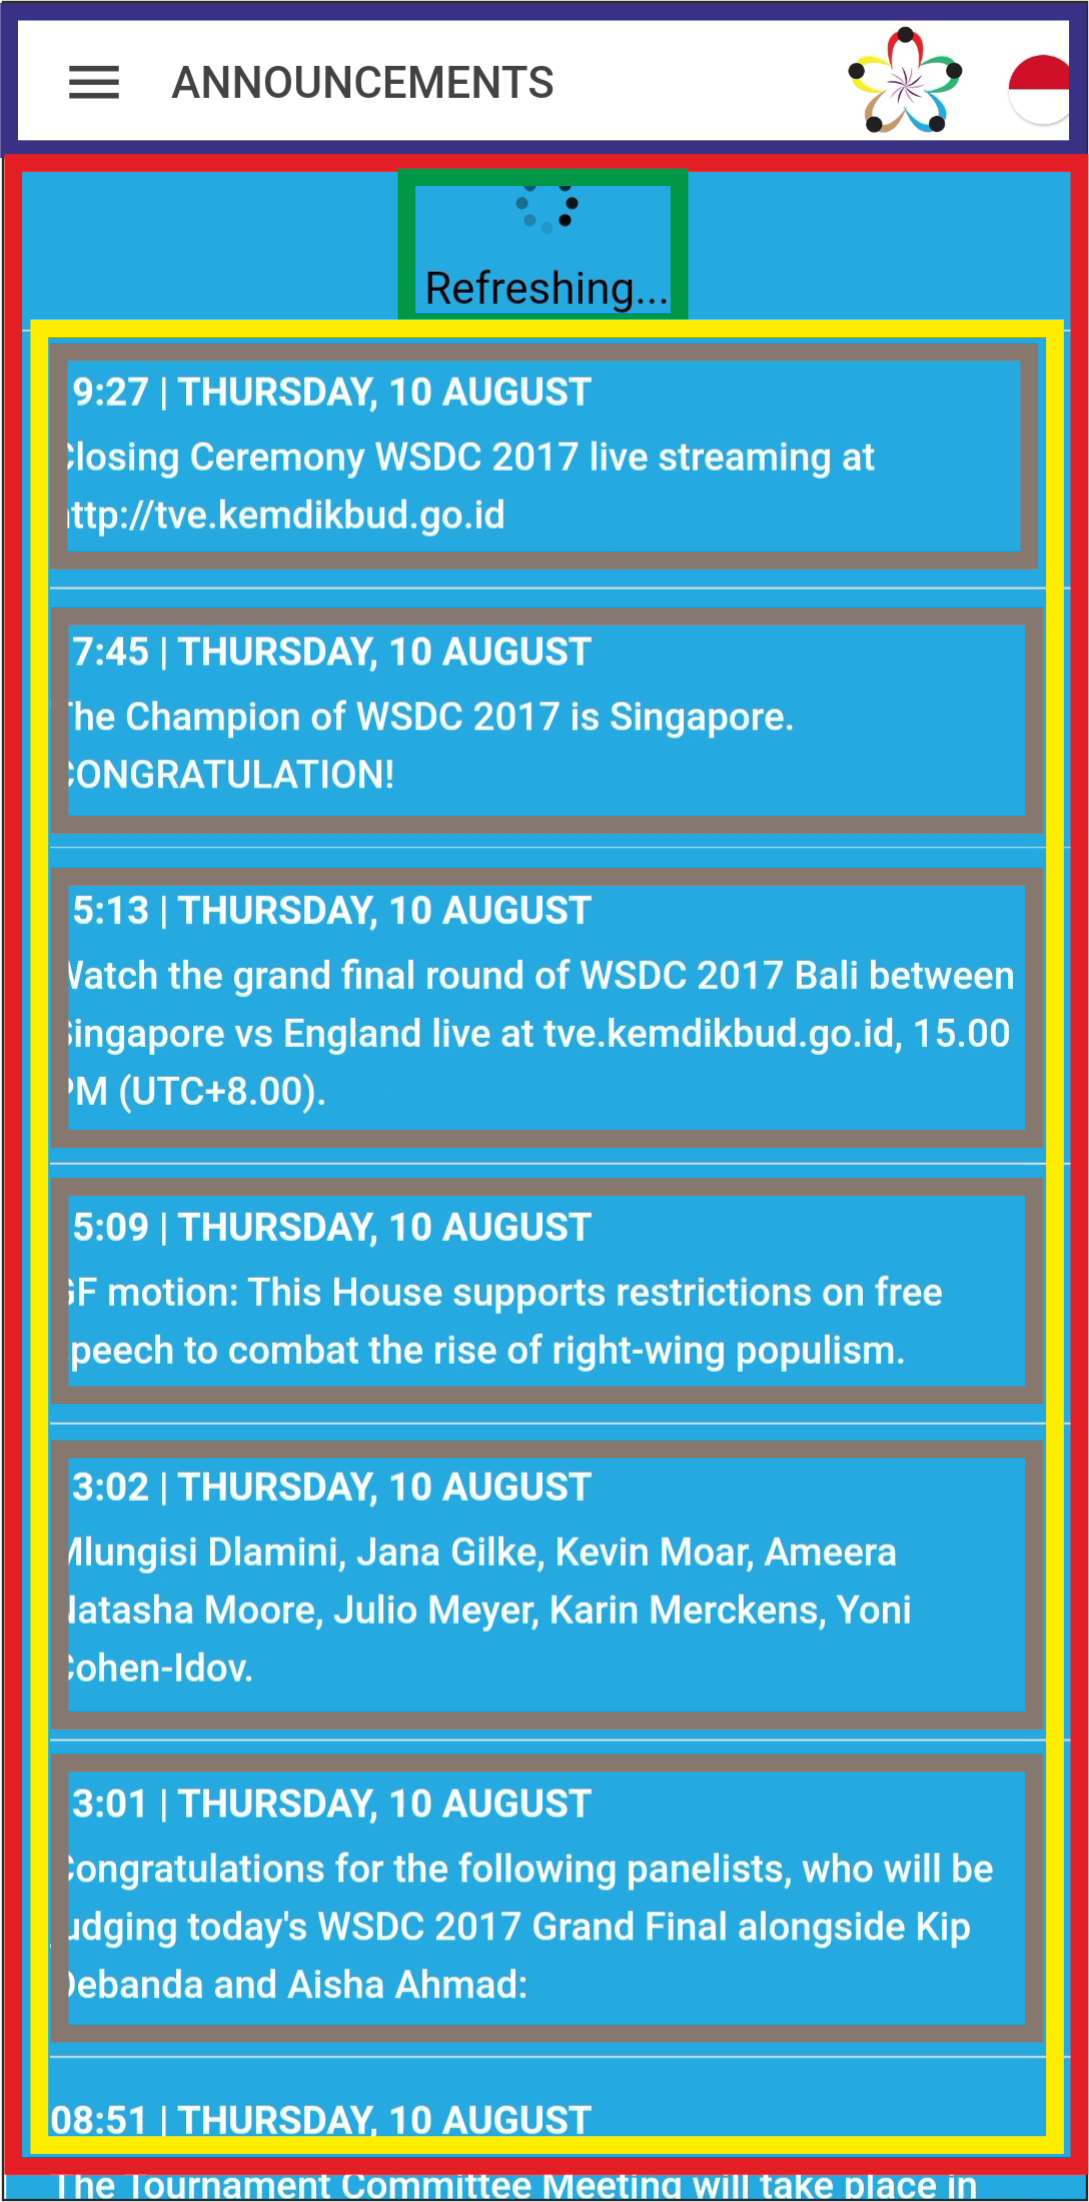
\includegraphics[scale=0.465]{Gambar/AnnouncementsPageWireframe.png}
         	\caption{Wireframe Komponen Announcements Aplikasi WSDC 2017 Bali terdahulu}
         	\label{fig:announcementsPageWireframe}
     	\end{subfigure}
     	\hspace*{0.5in}
     	\begin{subfigure}[b]{0.43\textwidth}
         	\centering
         	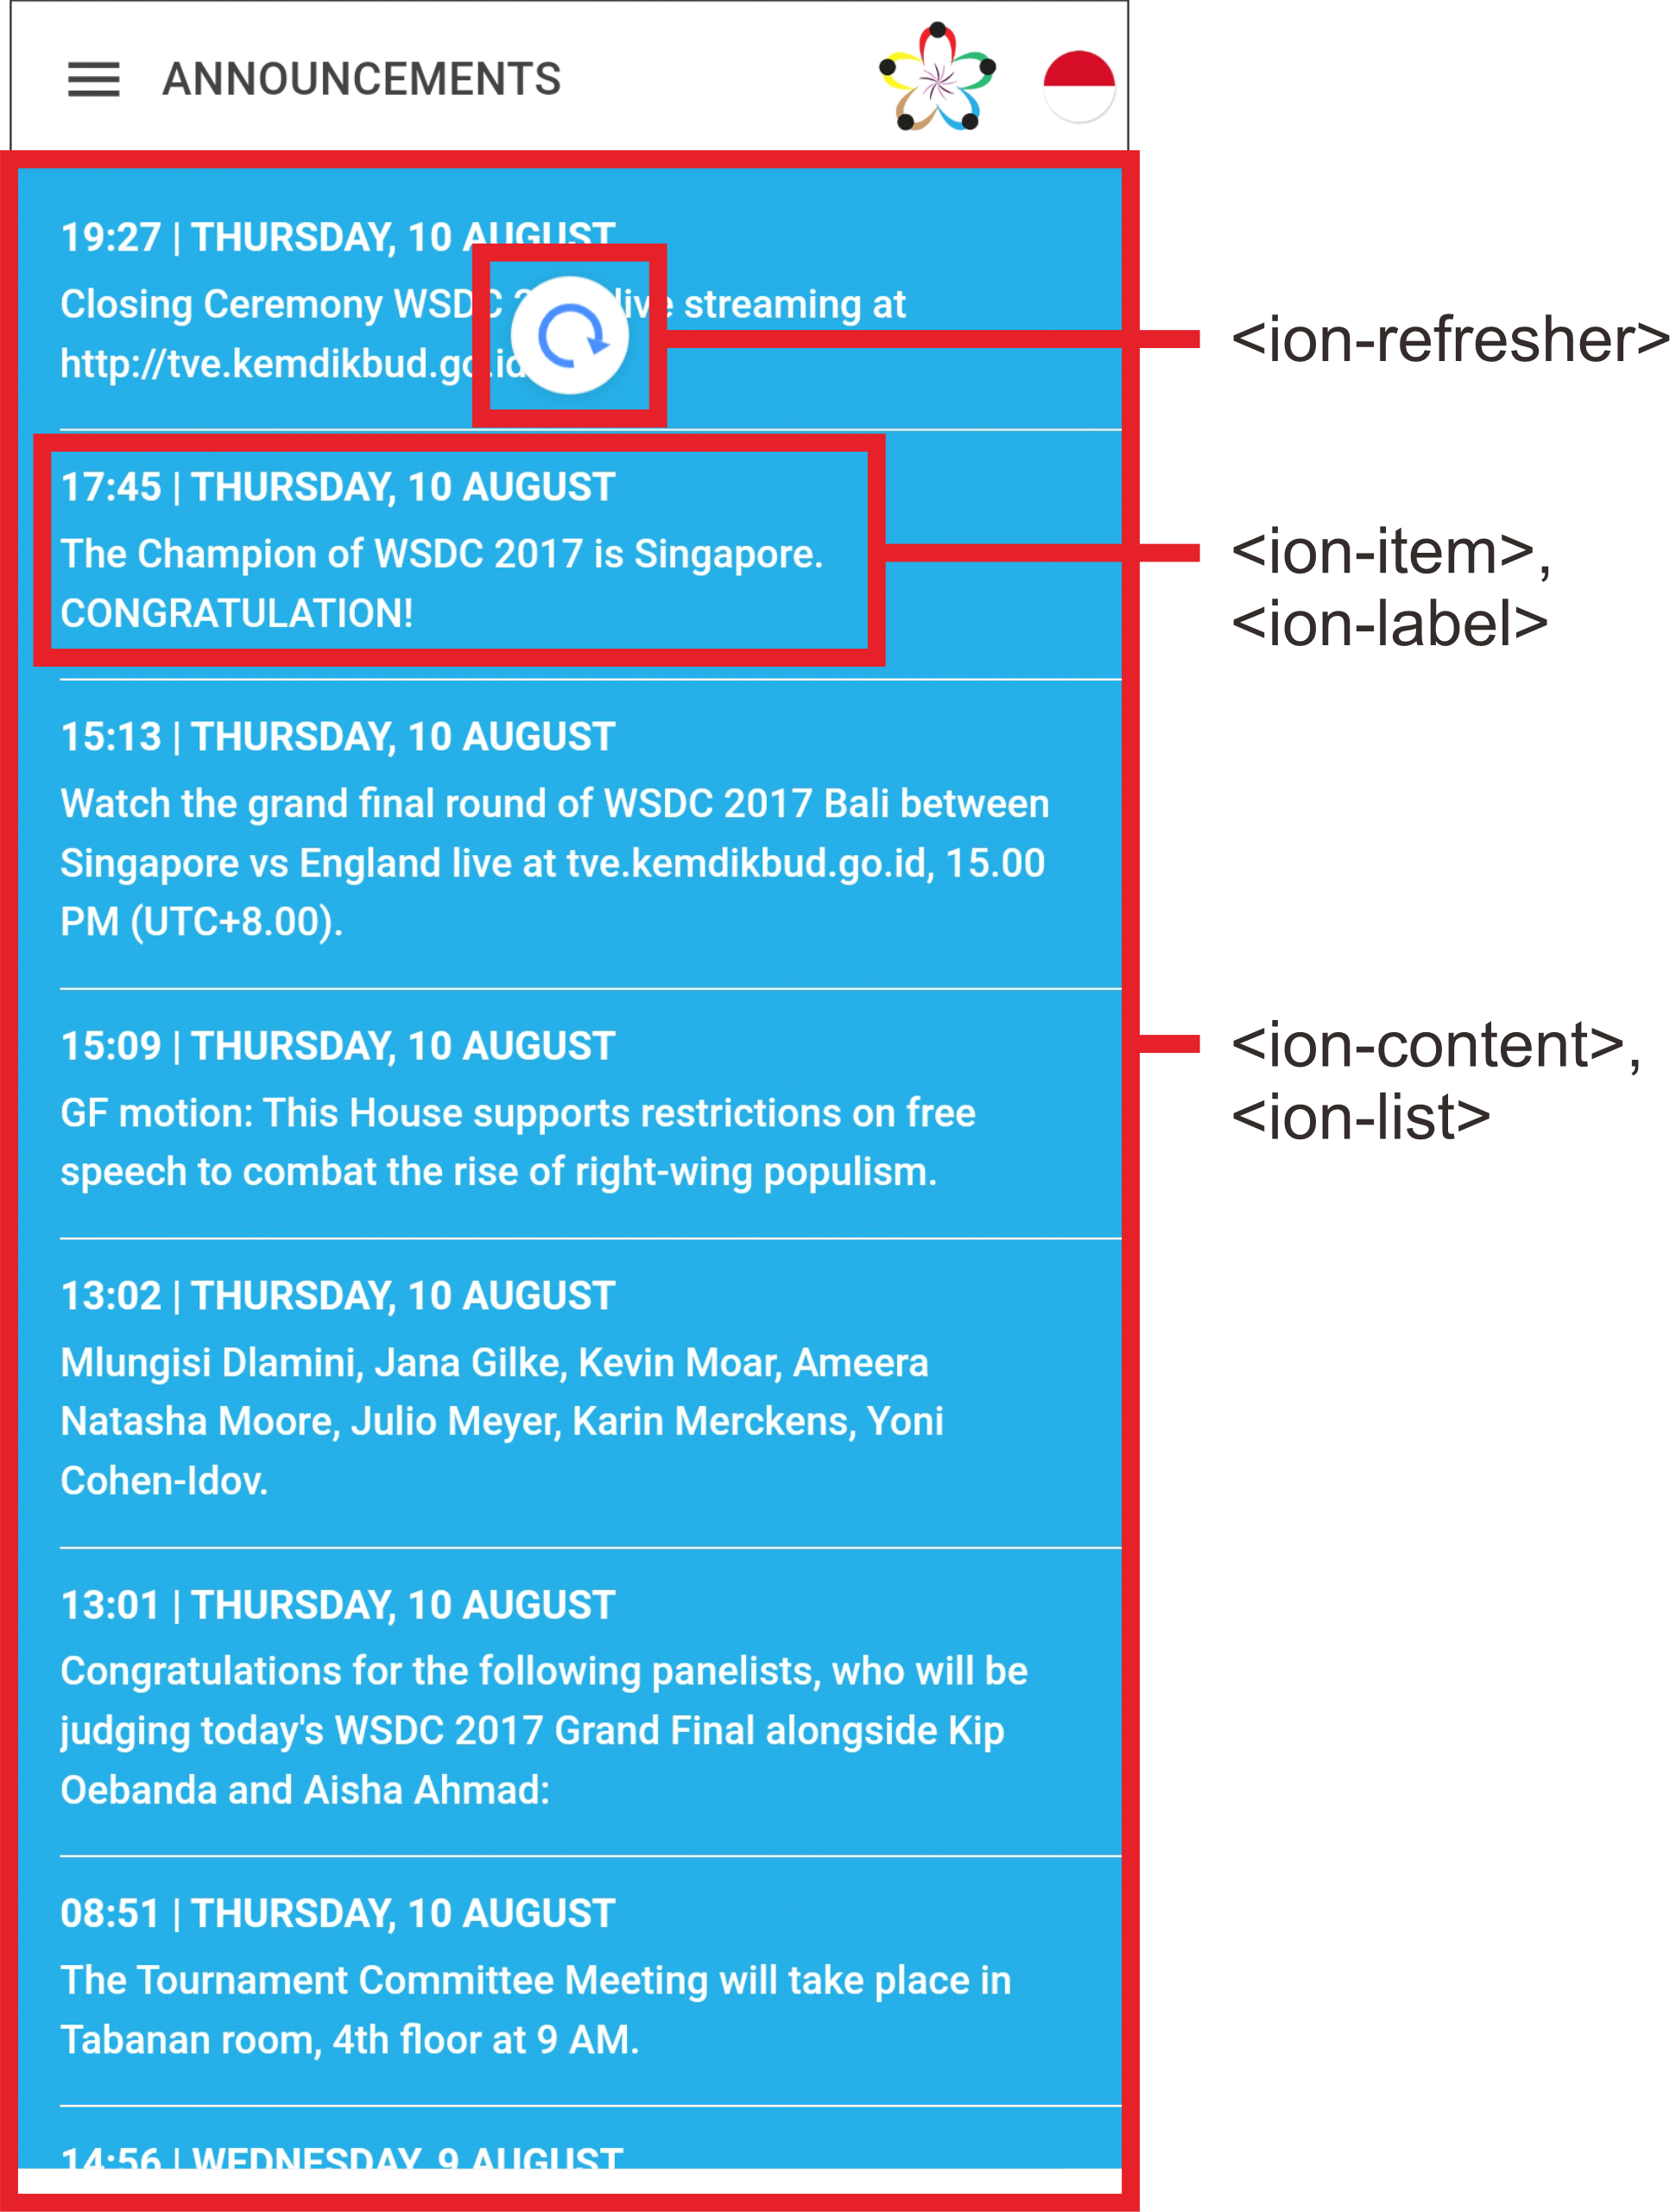
\includegraphics[scale=0.4]{Gambar/AnnouncementsPageKini.png}
         	\caption{UI Component Komponen Announcements Aplikasi WSDC 2017 Bali terbaru}
         	\label{fig:AnnouncementsPageKini}
     	\end{subfigure}
        \caption{Komponen Announcements pada Aplikasi WSDC 2017 Bali}
        \label{fig:UIComponent1}
	\end{figure}
	
	\begin{enumerate}
		\item Analisis pada Aplikasi WSDC 2017 Bali terdahulu \\
		Komponen ini digunakan untuk menampilkan halaman \textit{Announcement} pada aplikasi. Komponen ini memiliki sebuah \textit{file} TypeScript untuk mengatur keseluruhan halaman. Di dalam \textit{file} announcement.ts terdapat sebuah \textit{decorator} @Component untuk komponen (Kode~\ref{lst:componentannouncement}). Di dalam decorator ini terdapat CSS \textit{selector} untuk memilih CSS yang akan digunakan, serta \textbf{templateUrl} untuk mendefinisikan ekxternal HTML \textit{template} yang akan digunakan. \textit{Template} HTML yang digunakan adalah \textit{file} announcement.html. 
		\newpage
\begin{lstlisting}[label={lst:componentannouncement}, caption=@Component pada annoncement.ts]
@Component({
  selector: 'page-announcements',
  templateUrl: 'announcements.html'
})
\end{lstlisting} 
	Pada komponen ini terdapat sebuah kelas AnnouncementsPage yang berisi beberapa \textit{method} yang akan digunakan di dalam aplikasi. \textit{Method} pada kelas ini diataranya adalah sebagai berikut:
	\begin{itemize}
		\item ionViewDidLoad() \\
		\textit{Method} ini merupakan sebuah \textit{lifecycle event} yang dijalankan saat halaman \textit{announcement} telah dimuat. \textit{Event} ini hanya berjalan satu kali, jadi jika sudah melakukan chache terhadap halaman ini, maka ionViewDidLoad() tidak akan berjalan lagi. \textit{Lifecycle event} ini berguna untuk melakukan pengaturan awal, yaitu untuk memuat data \textit{announcement} dari \textit{storage}, dan menyimpannya di dalam variabel lokal. 
		\item doRefresh(refresher) \\
		\textit{Method} ini berfungsi untuk melakukan penyegaran ulang pada halaman \textit{announcement} untuk mendapatkan data \textit{announcement} terbaru di dalam server, kemudian menyimpannya ke dalam penyimpanan Ionic. \textit{Method} ini memiliki sebuah parameter refresher, yang berisi sebuah CustomEvent dari penyegaran ulang yang dilakukan.
		\item presentConnectionAlert() \\
		\textit{Method} ini digunakan ketika method doRefresh() mengalami \textit{error}, yang kemudian memunculkan \textit{toast}.
		\item formatDatetime(sqlDatetime: string) \\
		\textit{Method} ini berfungsi untuk membuat format tanggal dan waktu. \textit{Method} ini memiliki sebuah parameter, yaitu sqlDatetime yang bertipe \textit{string}, yang merupakan sebuah \textit{string} tanggal dengan format ``tahun-bulan-hari jam-menit-detik". \textit{Method} ini akan mengembalikan sebuah teks yang berisi waktu, tanggal dan bulan.
	\end{itemize}

	\textit{File} announcement.html digunakan untuk menampilkan halaman \textit{announcemnet}. Terdapat beberapa komponen yang disediakan oleh Ionic Framework, yang diimplementasikan ke dalam halaman \textit{announcement}. Diantaranya adalah sebagai berikut:	
	
	\begin{itemize}
		\item \textit{Header} \\
		Pada \textit{header} dari halaman \textit{announcement}, digunakan beberapa \textit{tag} dari komponen yang disediakan oleh Ionic Framework (Kode~\ref{lst:headerannouncement}). Yaitu \textit{tag} \texttt{<ion-header>} yang merupakan komponen \textit{parent} yang menampung komponen \textit{toolbar} yang ditandai dengan warna biru pada gambar ~\ref{fig:announcementsPageWireframe}. Di dalam \textit{tag} tersebut terdapat \textit{tag} pendukung, seperti \texttt{<ion-navbar>}, \texttt{<button>} sebagai tombol untuk membuka \textit{sidemenu}, \texttt{<ion-icon>} untuk menampilkan icon dari tombol pada \textit{tag button}, dan \texttt{<ion-title>} untuk menampilkan judul dari halaman, yaitu \textit{Announcement}, pada \textit{navbar}.\newpage
\begin{lstlisting}[label={lst:headerannouncement}, caption=\textit{Header} pada Halaman \textit{Annoncement}]
<ion-header>
  <ion-navbar>
    <button ion-button menuToggle>
      <ion-icon name="menu"></ion-icon>
    </button>
    <ion-title>Announcements</ion-title>
  </ion-navbar>
</ion-header>
\end{lstlisting} 

		\item \textit{Content} \\
		Konten pada halaman \textit{announcement} yang ditandai dengan kotak berwarna merah pada gambar~\ref{fig:announcementsPageWireframe} disusun menggunakan \textit{tag} \texttt{ion-content>} (Kode~\ref{lst:contentannouncement}). \textit{Tag} ini berisi beberapa \textit{tag} lain, yaitu \textit{tag} \texttt{<ion-refresher>}, yang ditandai dengan kotak hijau, yang akan menampilkan simbol \textit{refresh} saat pengguna menyegarkan halaman dengan cara melakukan \textit{swipe} dari atas ke bawah layar. Kemudian terdapat \textit{tag} \texttt{<ion-list>} yang ditandai dengan kotak kuning, berfungsi untuk menampilkan baris. Baris-baris tersebut diisi menggunakan \textit{tag} \texttt{<ion-item>} yang ditandai dengan kotak berwarna hitam, digunakan untuk menyimpan teks yang berisi tanggal, dan pesan pengumuman.

		
\begin{lstlisting}[label={lst:contentannouncement}, caption=\textit{Content} pada Halaman \textit{Annoncement}]
<ion-content>
  <ion-refresher (ionRefresh)="doRefresh($event)">
    <ion-refresher-content pullingIcon="arrow-dropdown" pullingText="Pull to refresh" refreshingSpinner="circles" refreshingText="Refreshing...">
    </ion-refresher-content>
  </ion-refresher>
  <ion-list>
    <ion-item text-wrap *ngFor="let announcement of announcements">
      <h3>{{formatDatetime(announcement.localtime)}}</h3>
      <p>{{announcement.message}}</p>
    </ion-item>
  </ion-list>
</ion-content>
\end{lstlisting} 
	\end{itemize}
	
		\item Perancangan Aplikasi WSDC 2017 Bali terbaru \\
		Pada komponen \textit{announcement}, terdapat beberapa UI Component yang akan diimplementasikan seperti pada gambar~\ref{fig:AnnouncementsPageKini}, diantaranya adalah sebagai berikut:
	\begin{itemize}
		\item \textit{Content} \\
		Komponen ini akan digunakan sebagai penyedia area konten yang digunakan untuk mengontrol area yang dapat digulir dan menampilkan isi konten dari halaman \textit{announcement}. UI Component \textit{Content} dengan \textit{tag} \texttt{<ion-content>} pada Ionic Framework versi 6 tidak mengalami perubahan dari Ionic Framework versi 3. 
		\newpage
		\item \textit{Refresher} \\
		\textit{Refresher} menyediakan fungsionalitas  pull-to-refresh pada komponen \textit{content}. UI Component \textit{Refresher} dengan \textit{tag} \texttt{<ion-refresher>} dan \texttt{<ion-refresher-content>} pada Ionic Framework versi 6 tidak mengalami perubahan dari Ionic Framework versi 3.

		\item \textit{List} \\
		\textit{List} dengan \textit{tag} \texttt{<ion-list>} akan terdiri dari beberapa baris item \texttt{<ion-item>} yang berisi label \texttt{<ion-label>}. UI Component \textit{List} dengan \textit{tag} \texttt{<ion-list>}, \texttt{<ion-item>} dan \texttt{<ion-label>} pada Ionic Framework versi 6 tidak mengalami perubahan dari Ionic Framework versi 3.
		
		\item \textit{Item} \\
		\textit{Item} dengan \textit{tag} \texttt{<ion-item>} sejak Ionic 4 mengalami perubahan dibandingkan pada Ionic 3, yaitu wajib menambahkan \textit{label} dengan \textit{tag} \texttt{<ion-label>}. Pada aplikasi WSDC 2017 Bali saat ini yang menggunakan Ionic 3, tidak terdapat \textit{tag} \texttt{<ion-label>} pada \texttt{<ion-item>} (Kode~\ref{lst:itemWSDCOld}). Sedangkan sesuai dengan ketentuan yang berlaku, pada aplikasi yang akan dibangun yang menggunakan Ionic 6, akan menggunakan \textit{tag} \texttt{<ion-label>} di dalam \texttt{<ion-item>} (Kode~\ref{lst:itemWSDCNew}).
		
\begin{lstlisting}[label={lst:itemWSDCOld}, caption=\textit{Tag} \texttt{<ion-item>} dengan Ionic 3 di Aplikasi WSDC 2017 Bali Saat Ini]
<ion-item text-wrap *ngFor="let announcement of announcements">
	<h3>{{formatDatetime(announcement.localtime)}}</h3>
    <p>{{announcement.message}}</p>
</ion-item>
\end{lstlisting}

\begin{lstlisting}[label={lst:itemWSDCNew}, caption=\textit{Tag} <ion-item> dengan Ionic 6 di Aplikasi WSDC 2017 Bali yang Akan dibuat]
<ion-item color="wsdc-blue" *ngFor="let announcement of announcements; let i = index">
    <ion-label>
    	<h3>{{ formatDatetime(announcement.localtime) }}</h3>
        <p>{{ announcement.message }}</p>
    </ion-label>
</ion-item>
\end{lstlisting}
		
	\end{itemize}
	\end{enumerate}
	\item Komponen \textit{Draw} \\
	Komponen \textit{Draw} digunakan untuk melihat pembagian kubu proposisi dan oposisi dari tiap-tiap negara peserta.
	\begin{figure}[H]
    	\centering
     	\begin{subfigure}[b]{0.43\textwidth}
        	\centering
         	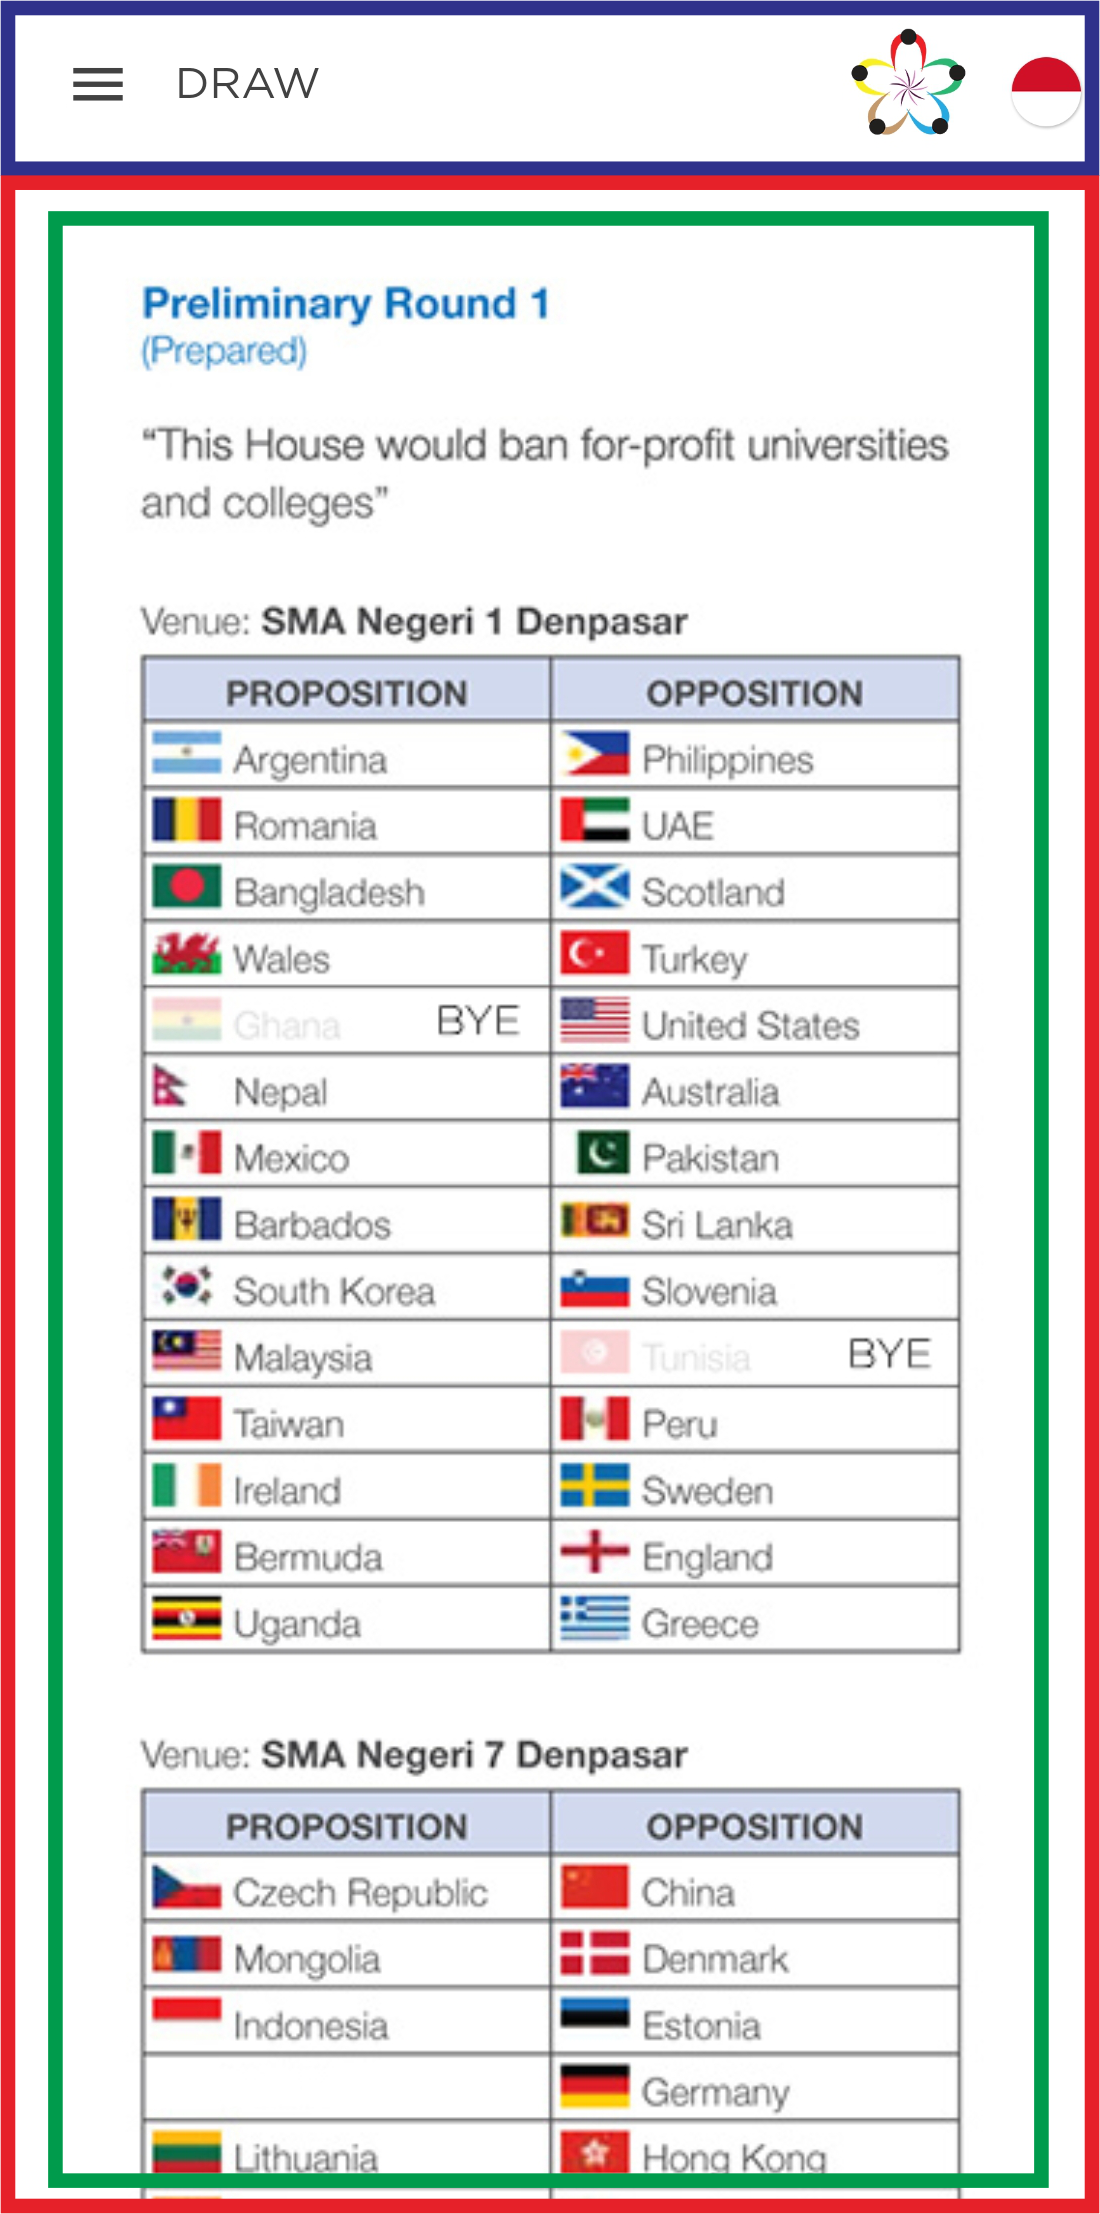
\includegraphics[scale=0.465]{Gambar/DrawPageWireframe.png}
         	\caption{Wireframe Komponen Draw Aplikasi WSDC 2017 Bali terdahulu}
         	\label{fig:drawPageWireframe}
     	\end{subfigure}
     	\hspace*{0.5in}
     	\begin{subfigure}[b]{0.43\textwidth}
         	\centering
         	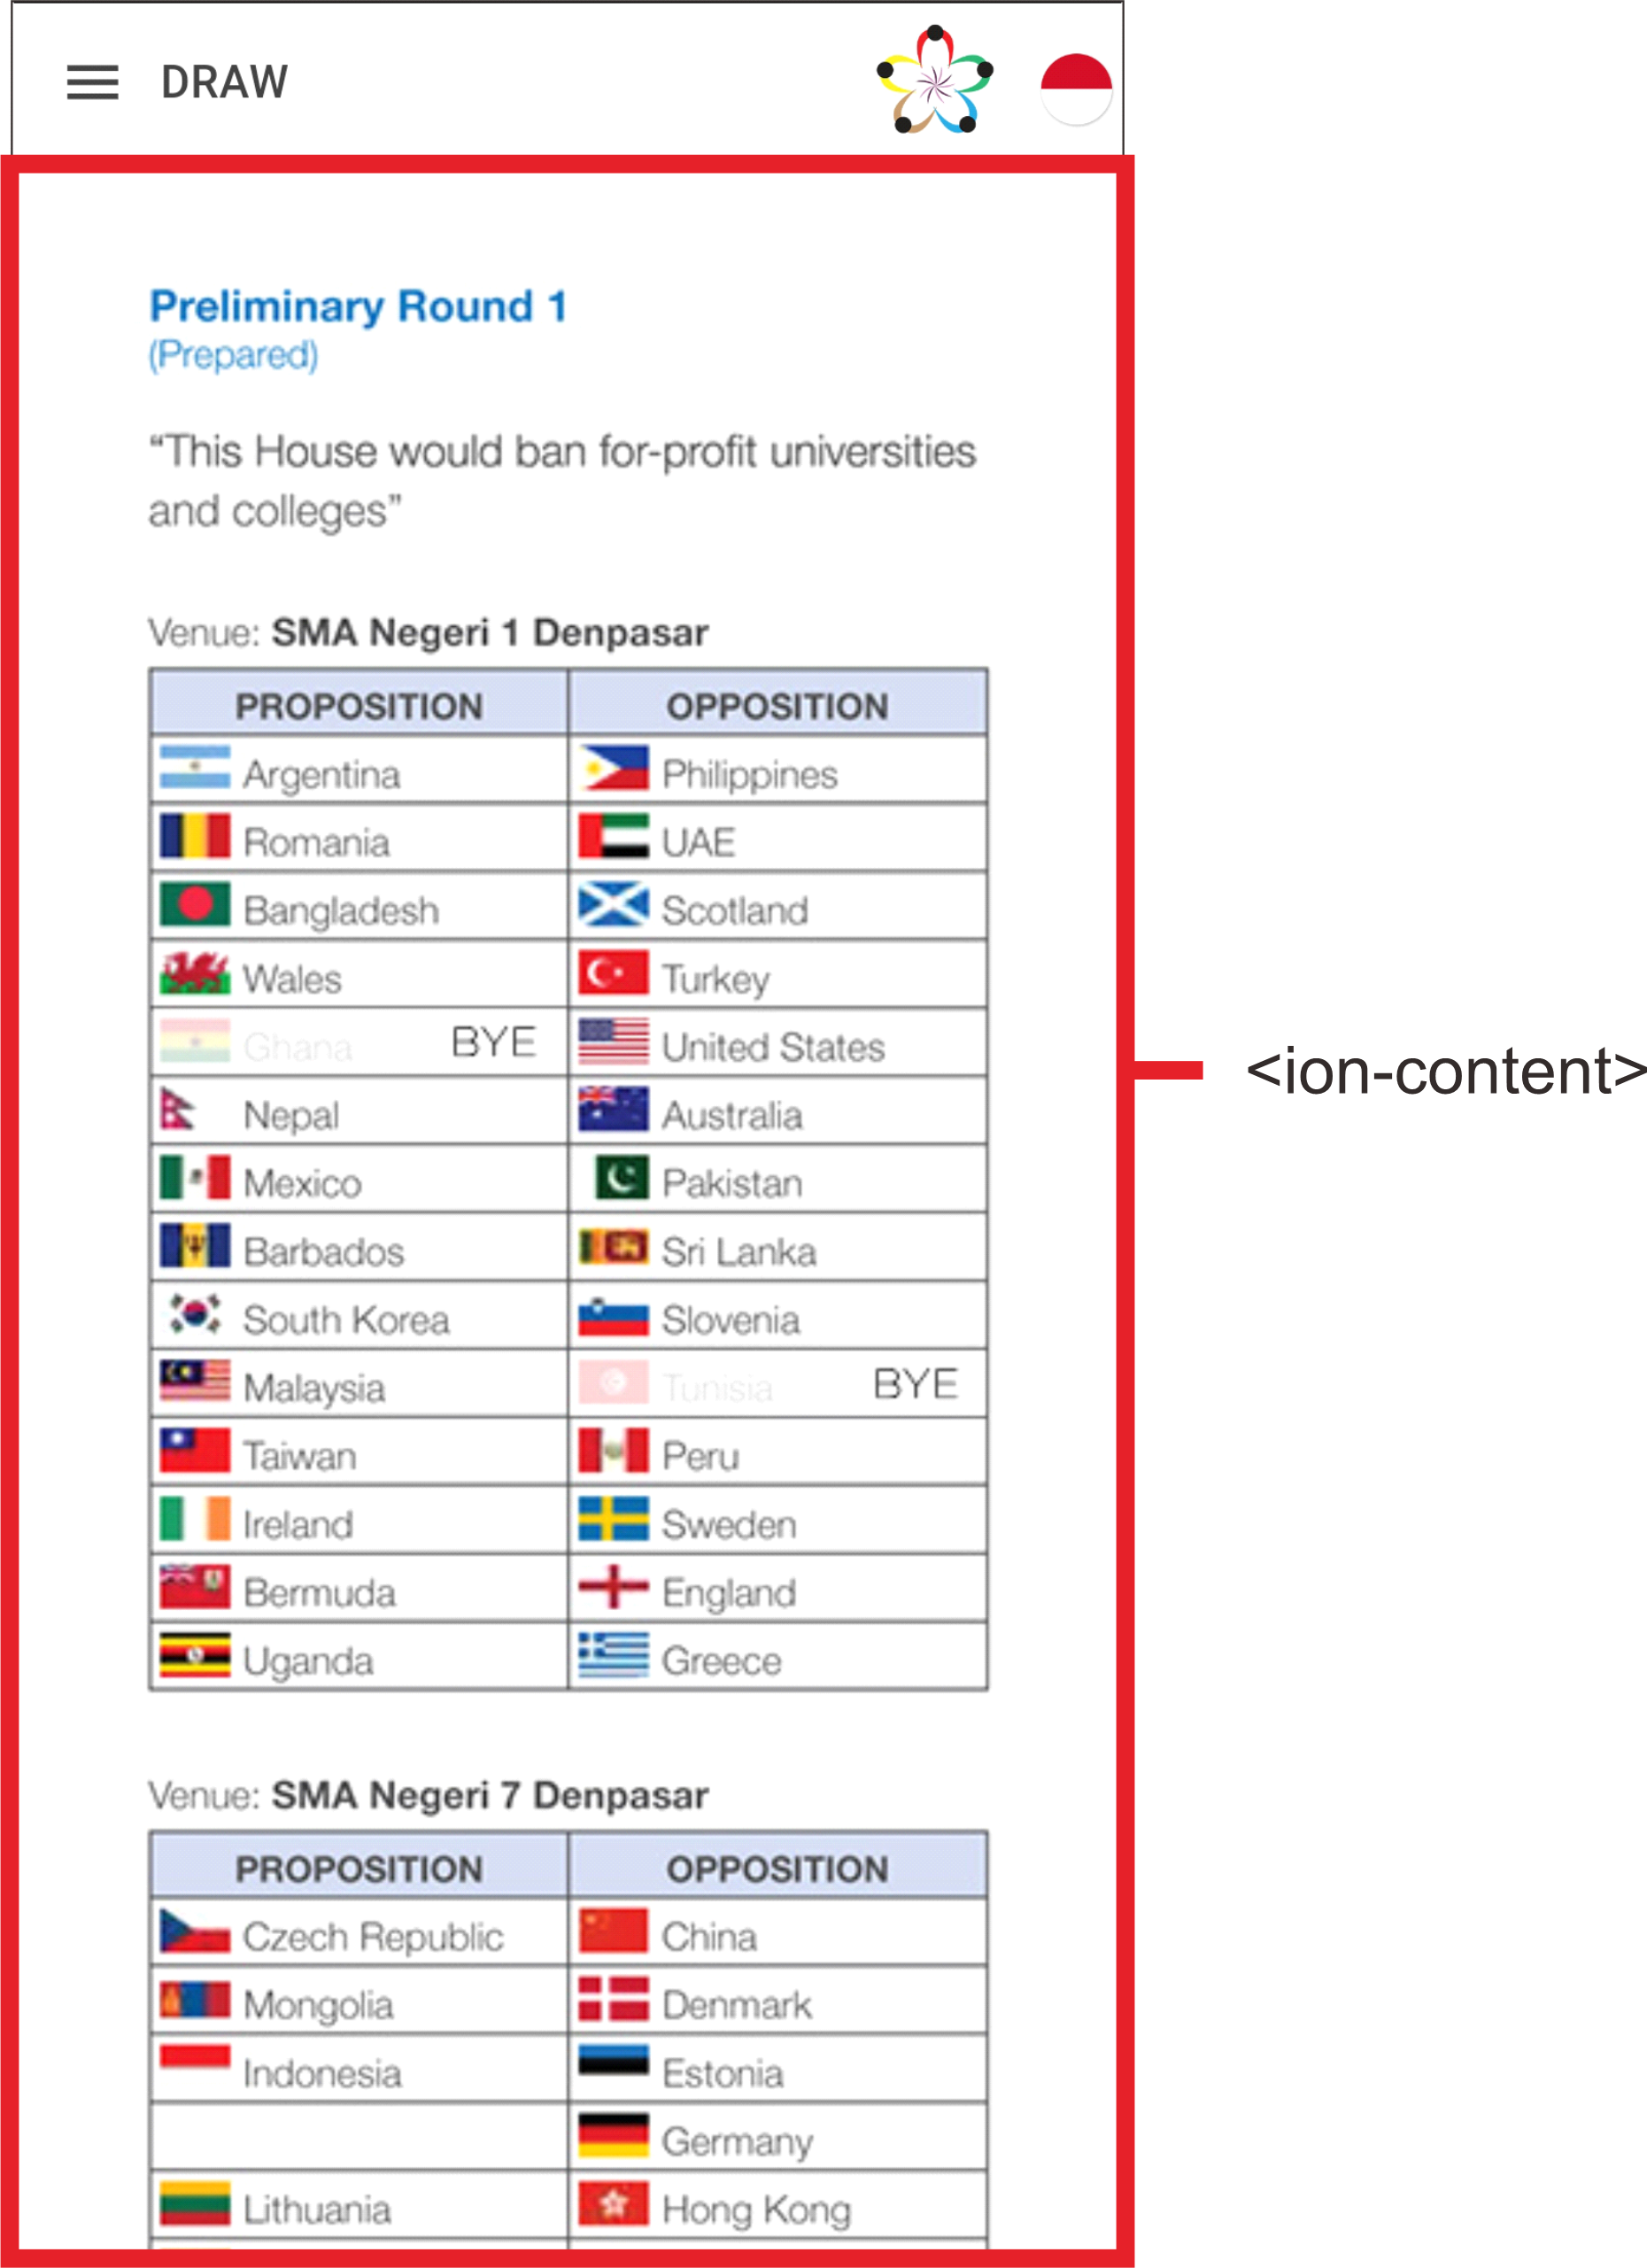
\includegraphics[scale=0.4]{Gambar/DrawPageKini.png}
         	\caption{UI Component Komponen Draw Aplikasi WSDC 2017 Bali terbaru}
         	\label{fig:DrawPageKini}
     	\end{subfigure}
        \caption{Komponen Draw pada Aplikasi WSDC 2017 Bali}
        \label{fig:UIComponent1}
	\end{figure}
	\begin{enumerate}
		\item Analisis pada Aplikasi WSDC 2017 Bali terdahulu \\
		Terdapat \textit{file} TypeScript, draw.ts, yang berfungsi untuk mengatur keseluruhan halaman. Di dalam \textit{flie} tersebut terdapat \textit{decorator} @Component (Kode~\ref{lst:componendraw}) dan \textit{decorator} @ViewChild (Kode~\ref{lst:viewchilddraw}). Pada \textit{decorator} @Component, terdapat CSS \textit{selector} untuk memilih CSS mana yang akan digunakan, serta \textbf{templateUrl} untuk mendefinisikan ekxternal HTML \textit{template} halaman \textit{Draw}yang akan digunakan, yaitu draw.html. @ViewChild digunakan untuk memanggil elemen dari DOM untuk meamanggil komponen API ke dalam TypeScript, yaitu pada komponen \textit{draw} adalah drawIFrame yang berada di \textit{file} draw.html.
\begin{lstlisting}[label={lst:componendraw}, caption=@Component pada draw.ts]
@Component({
  selector: 'page-draw',
  templateUrl: 'draw.html'
})
\end{lstlisting} 

\begin{lstlisting}[label={lst:viewchilddraw}, caption=@ViewChild pada draw.ts]
@ViewChild('drawIFrame') drawIFrame: ElementRef;
\end{lstlisting} 

	Terdapat kelas DrawPage yang berisi beberapa \textit{method} yang akan digunakan di dalam aplikasi, diataranya adalah sebagai berikut:
	
	\begin{itemize}
		\item ionViewDidLoad() \\
		\textit{Method} ini merupakan sebuah \textit{lifecycle event} yang dijalankan saat halaman \textit{draw} telah dimuat. \textit{Event} ini hanya berjalan satu kali, jadi jika sudah melakukan chache terhadap halaman ini, maka ionViewDidLoad() tidak akan berjalan lagi. \textit{Lifecycle event} ini berguna untuk melakukan pengaturan awal, yaitu untuk memuat data \textit{draw} dari \textit{storage}, kemudian data tersebut dimasukkan ke dalam \textit{child} drawIFrame. Terakhir, method ini akan memanggil method presentLoading().
		
		\item presentLoading() \\
		\textit{Method} ini berfungsi untuk menampilkan sebuah \textit{overlay} yang menunjukkan sebuah pesan dan indikator pemuatan saat pertama kali halaman \textit{draw} dimuat. Karena \textit{overlay} ini muncul di atas konten aplikasi, maka aktivitas pengguna akan diblokir untuk sementara sampai seluruh halaman dimuat, yaitu sampai \textit{method} onDrawIframeLoad() selesai.
		\item onDrawIframeLoad() \\
		\textit{Method} ini merupakan sebuah \textit{template statement} dipanggil oleh \textit{event} di dalam \textit{tag} \texttt{<iframe>} pada draw.html yaitu \textit{event} (load). \textit{Method} ini berfungsi untuk menampilkan data yang telah diambil yang disimpan di dalam \textit{child} drawIFrame.
	\end{itemize}
	
	Terdapat \textit{file} draw.html yang digunakan untuk menampilkan tata letak dari halaman \textit{draw}. Terdapat beberapa komponen yang disediakan oleh Ionic Framework, yang diimplementasikan ke dalam halaman \textit{draw}. Diantaranya adalah sebagai berikut:	
	
	\begin{itemize}
		\item \textit{Header} \\
		\textit{Header} dari halaman \textit{draw} seperti pada gambar ~\ref{fig:drawPageWireframe} menggunakan \textit{tag} \texttt{<ion-header>} (Kode~\ref{lst:headerdraw}). \textit{Tag} tersebut merupakan komponen \textit{parent} yang menampung komponen navbar yang ditandai dengan kotak berwarna biru pada gambar~\ref{fig:drawPageWireframe}. Di dalam navbar tersebut, terdapat sebuah \textit{tag} \texttt{<button>} untuk memunculkan \textit{sidemenu}, \texttt{<ion-icon>} untuk menampilkan icon dari tombol pada \textit{tag button}, dan \textit{tag} \texttt{<ion-title>} sebagai judul dari halaman.

\begin{lstlisting}[label={lst:headerdraw}, caption=\textit{Header} pada draw.html]
<ion-header>
  <ion-navbar>
    <button ion-button menuToggle>
      <ion-icon name="menu"></ion-icon>
    </button>
    <ion-title>Draw</ion-title>
  </ion-navbar>
</ion-header>
\end{lstlisting} 

		\item \textit{Content} \\
		\textit{Content} dari halaman \textit{draw} seperti pada gambar~\ref{fig:drawPageWireframe} menggunakan \textit{tag} \texttt{<ion-content>} (Kode~\ref{lst:contentdraw}) yang ditandai menggunakan kotak berwarna merah. Di dalam \textit{tag} ini terdapat sebuah \textit{tag} \texttt{<iframe>} yang berisi hasil pengundian grup untuk peserta WSDC 2017 Bali, ditandai menggunakan kotak berwarna hijau. \textit{Tag} \texttt{<iframe>} menampilkan hasil dari \textit{method} onDrawIframeLoad() pada draw.ts.
		
\begin{lstlisting}[label={lst:contentdraw}, caption=\textit{Content} pada draw.html]
<ion-content>
  <iframe #drawIFrame (load)="onDrawIframeLoad()" class="iframe-fullscreen"></iframe>
</ion-content>
\end{lstlisting} 
	\end{itemize}\newpage
		\item Perancangan Aplikasi WSDC 2017 Bali terbaru \\
		Pada komponen \textit{draw}, terdapat sebuah UI Component, yaitu \textit{Content} seperti pada gambar~\ref{fig:DrawPageKini}. Komponen \textit{content} akan digunakan sebagai penyedia area konten yang digunakan untuk mengontrol area yang dapat digulir dan menampilkan isi konten dari halaman \textit{draw}. UI Component \textit{Content} dengan \textit{tag} \texttt{<ion-content>} pada Ionic Framework versi 6 tidak mengalami perubahan dari Ionic Framework versi 3. 
	\end{enumerate}
	
	\item Komponen \textit{Home} \\
	Komponen \textit{Home} digunakan untuk menampilkan halaman utama aplikasi WSDC 2017 Bali yang berisi pengumuman terbaru dari acara WSDC 2017 Bali, dan berita-berita terkait acara WSDC 2017 Bali.
	\begin{figure}[H]
    	\centering
     	\begin{subfigure}[b]{0.43\textwidth}
        	\centering
         	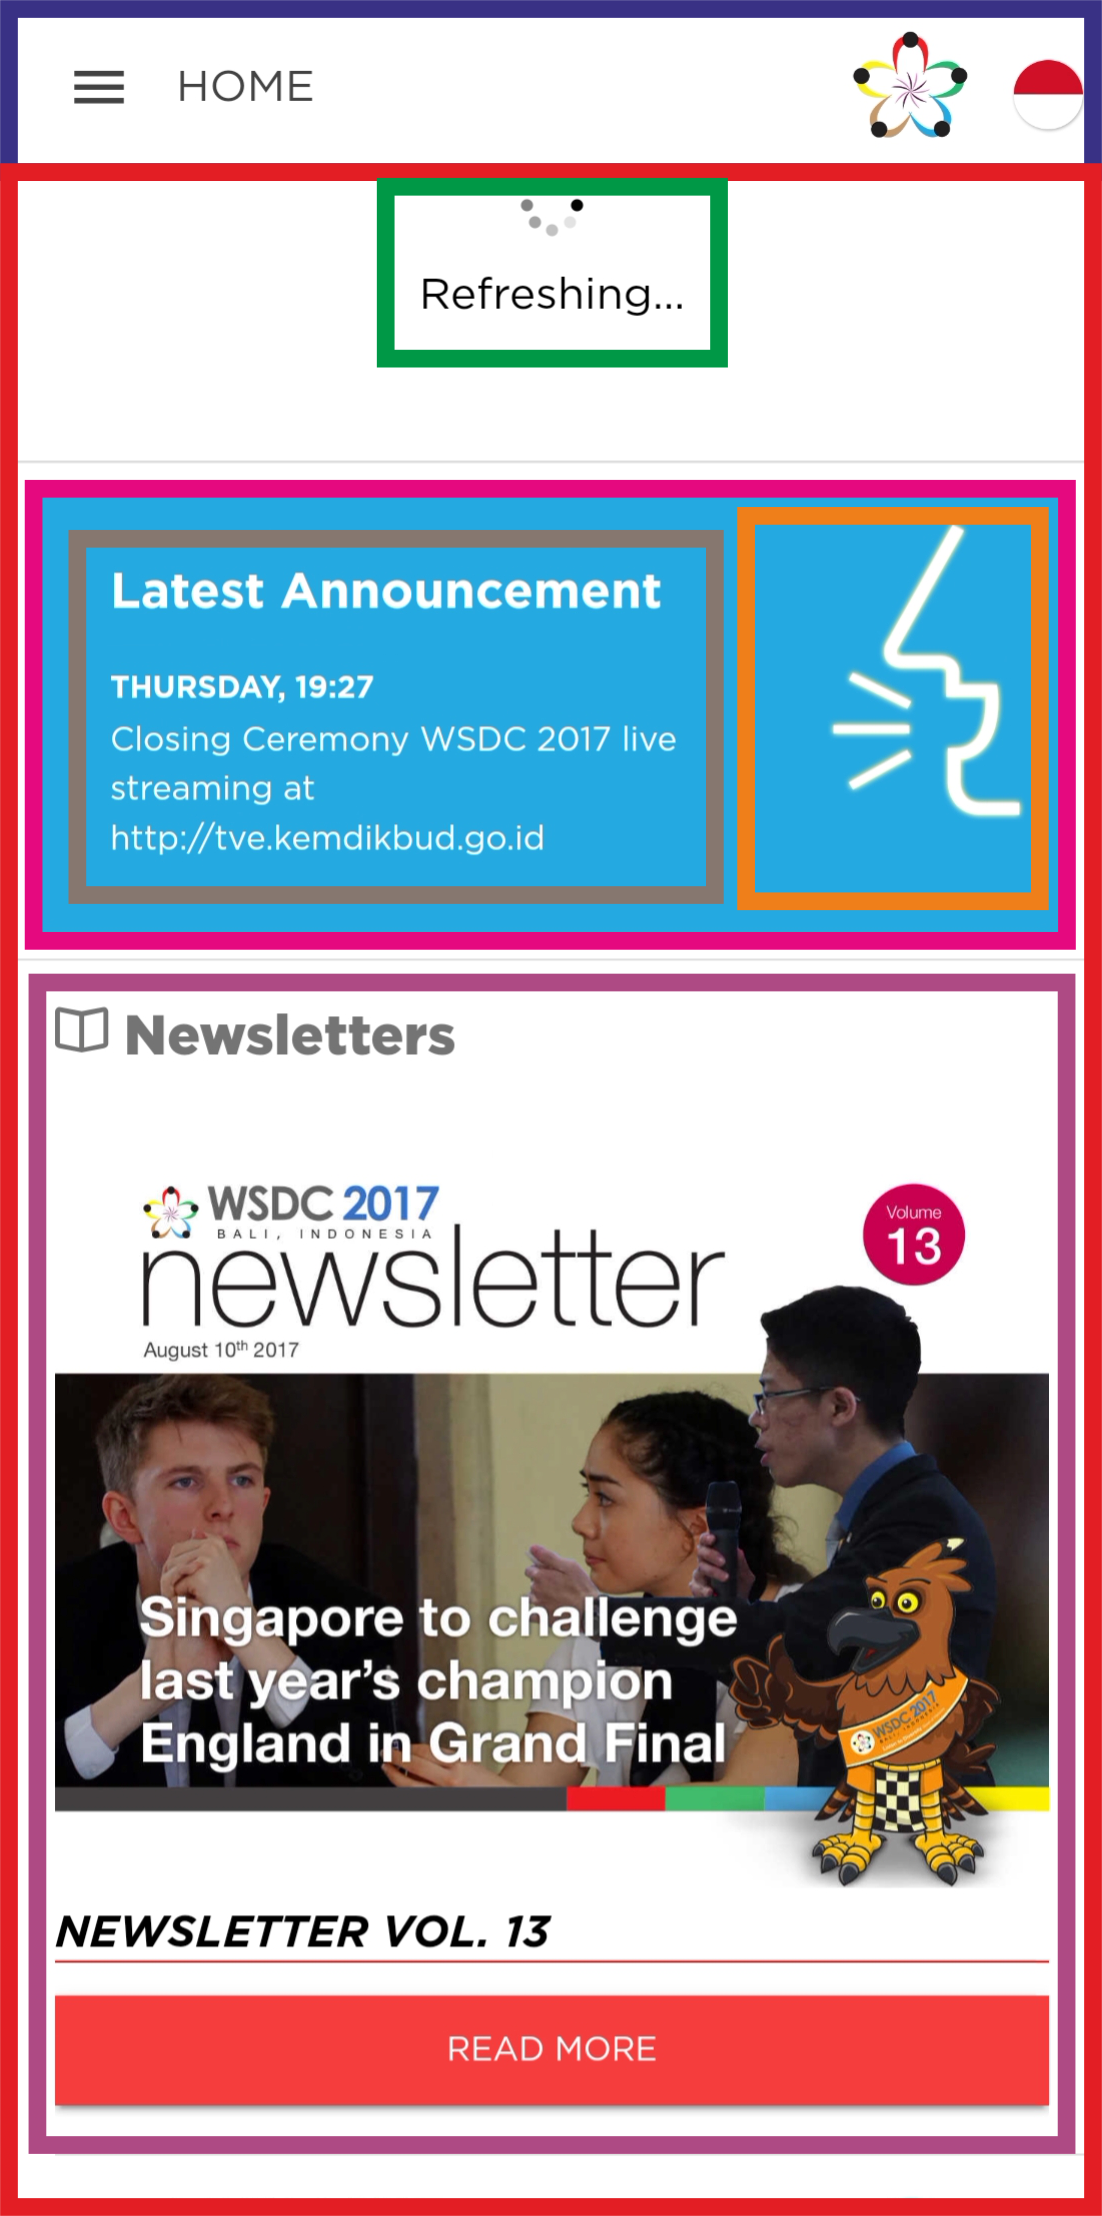
\includegraphics[scale=0.465]{Gambar/HomePageWireframe.png}
         	\caption{Wireframe Komponen Home Aplikasi WSDC 2017 Bali terdahulu}
         	\label{fig:homePageWireframe}
     	\end{subfigure}
     	\hspace*{0.5in}
     	\begin{subfigure}[b]{0.43\textwidth}
         	\centering
         	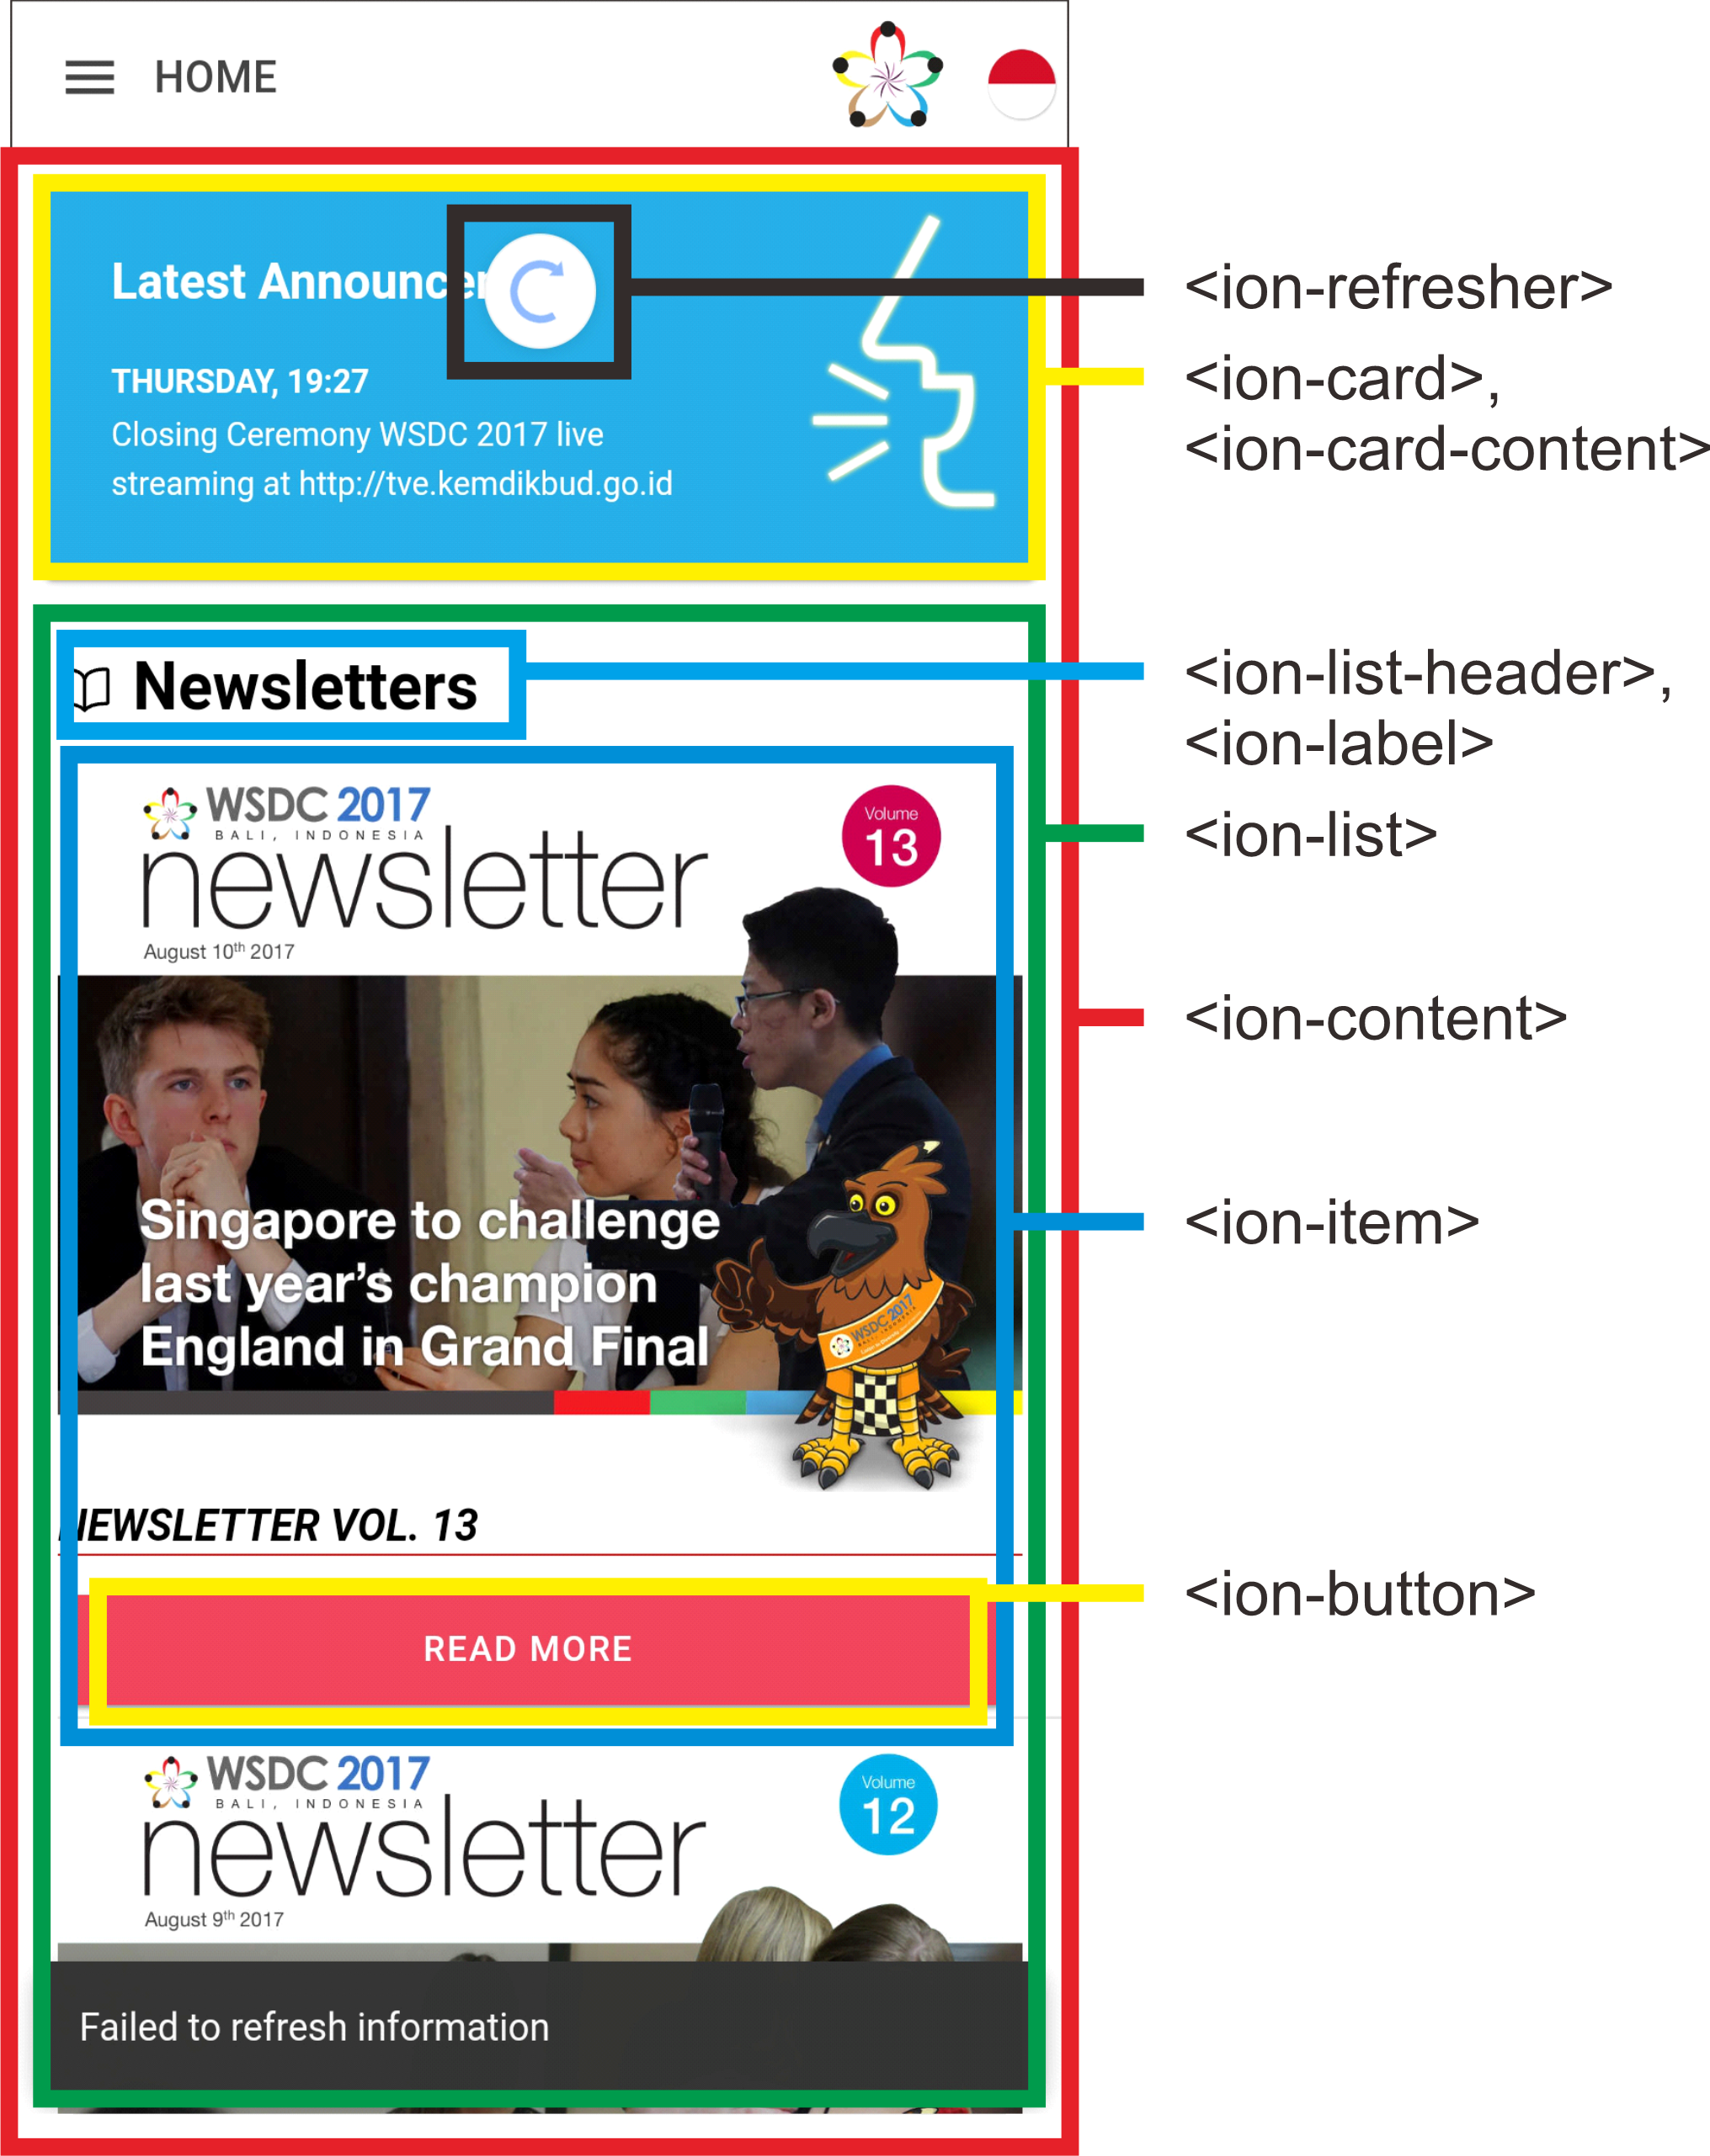
\includegraphics[scale=0.4]{Gambar/HomePageKini.png}
         	\caption{UI Component Komponen Home Aplikasi WSDC 2017 Bali terbaru}
         	\label{fig:HomePageKini}
     	\end{subfigure}
        \caption{Komponen Home pada Aplikasi WSDC 2017 Bali}
        \label{fig:UIComponent1}
	\end{figure}
	\begin{enumerate}
		\item Analisis pada Aplikasi WSDC 2017 Bali terdahulu \\
		Komponen ini memiliki sebuah \textit{file} TypeScript untuk mengatur keseluruhan halaman. Di dalam \textit{file} home.ts terdapat sebuah \textit{decorator} @Component untuk komponen (Kode~\ref{lst:componenthome}). Di dalam decorator ini terdapat CSS \textit{selector} untuk memilih CSS yang akan digunakan, serta templateUrl untuk mendefinisikan ekxternal HTML \textit{template} yang akan digunakan. \textit{Template} HTML yang digunakan adalah \textit{file} home.html.

\begin{lstlisting}[label={lst:componenthome}, caption=@Component pada home.ts]
@Component({
  selector: 'page-home',
  templateUrl: 'home.html'
})
\end{lstlisting}	
	\newpage
	Komponen \textit{Home} merupakan komponen yang menjadi rootPage dari aplikasi ini, yang dimasukan di dalam \textit{file} app.component.ts. Maka dari itu, saat pertama kali aplikasi dijalankan, komponen \textit{home}-lah yang pertama kali ditampilkan di dalam layar. rootPage di dalam \textit{file} app.component.ts akan memanggil komponen \textit{home}, yang kemudian \textit{file} home.ts akan berjalan. 
	
	Di dalam \textit{file} ini terdapat sebuah kelas HomePage yang berisi beberapa \textit{method}, diantaranya adalah sebagai berikut:
	
	\begin{itemize}
		\item ionViewDidLoad() \\
		\textit{Method} ini merupakan sebuah \textit{lifecycle event} yang dijalankan saat halaman \textit{home} telah dimuat. \textit{Event} ini hanya berjalan satu kali, jadi jika sudah melakukan chache terhadap halaman ini, maka ionViewDidLoad() tidak akan berjalan lagi. \textit{Lifecycle event} ini berguna untuk melakukan pengaturan awal, yaitu untuk untuk mengambil keseluruhan data aplikasi yang ada di dalam penyimpanan. Dengan memanfaatkan fitur \textit{storage} yang dimiliki oleh Ionic Framework, \textit{method} ini akan mengecek apakah sudah ada data dengan format .json yang berisi keseluruhan data aplikasi di dalam penyimpanan. Data tersebut berisi data \textit{announcements}, \textit{newsletters}, \textit{schedule}, \textit{venues}, \textit{draws}, dan info. Jika data tersebut tidak ditemukan, maka akan diambil dari \textit{file} wsdc-data.json dari aset lokal menggunakan HTTP API yang disediakan oleh Angular, yaitu HTTPClient, kemudian dimasukan ke dalam penyimpanan. Hal ini bertujuan jika pengguna tidak memiliki koneksi internet pada saat pemasangan aplikasi, aplikasi masih bisa dijalankan dan menampilkan halaman-halaman yang tidak kosong karena data diambil dari aset lokal.
		
		Setelah itu, \textit{method} ini mengambil data terbaru dari server dengan menggunakan Angular HTTPClient. Jika sudah melewati batas waktu, dan aplikasi belum terhubung dengan server, maka \textit{method} ini akan memanggil \textit{method} showToast() yang akan menampilkan Toast yang berisi teks `Failed to refresh information'. Jika mengambil data dari server berhasil, maka data yang didapatkan dari server akan dimasukan ke dalam penyimpanan menggantikan data yang sudah ada di penyimpanan sebelumnya. Hal ini dilakukan dengan asumsi bahwa data yang terdapat di server merupakan data terbaru, sehingga data yang ada pada penyimpanan merupakan data lama dan harus diganti dengan data terbaru.
	
		\item launch(url: string) \\
		\textit{Method} ini merupakan sebuah \textit{template statement} dipanggil oleh \textit{event} di dalam tag \texttt{<button>} pada home.html yaitu \textit{event} (click). \textit{Method} ini memiliki sebuah parameter url yang bertipe \textit{stirng}. Parameter tersebut berisi url dari berita yang akan dilihat oleh penggunga. Untuk membuka berita pada url tersebut memanfaatkan \textit{plugin} InAppBrowser yang disediakan oleh Ionic. 
		
		\item formatDatetime(sqlDatetime: string) \\
		\textit{Method} ini berfungsi untuk membuat format tanggal dan waktu. \textit{Method} ini memiliki sebuah parameter, yaitu sqlDatetime yang bertipe \textit{string}, yang merupakan sebuah \textit{string} tanggal dengan format ``tahun-bulan-hari jam-menit-detik". \textit{Method} ini akan mengembalikan sebuah teks yang berisi waktu, tanggal dan bulan.\newpage
		\item doRefresh(refresher) \\
		\textit{Method} ini berfungsi untuk melakukan penyegaran ulang pada halaman \textit{home} untuk mendapatkan data \textit{home} terbaru di dalam server, kemudian menyimpannya ke dalam penyimpanan. \textit{Method} ini memiliki sebuah parameter refresher, yang berisi sebuah CustomEvent dari penyegaran ulang yang dilakukan. \textit{Method} ini akan melakukan pemanggilan kembali kepada server, dalam batas waktu tertentu. Jika batas waktu maksimal telah tercapai, sedangkan server belum juga memberi tanggapan, maka akan memanggil \textit{method} showToast() yang akan menampilkan sebuah Toast yang berisi teks `Failed to refresh information'. Jika berhasil untuk terhubung dengan server, \textit{method} ini akan menghapus data yang berada di penyimpanan, dan digantikan dengan data yang telah didapatkan dari server.
		\item showToast(message: string, duration: number = 3000) \\
		\textit{Method} ini berfungsi untuk memunculkan sebuah native Toast, yaitu sebuah \textit{popup} teks, dengan memanfaatkan UI Component milik Ionic Framework. \textit{Method} ini menerima parameter berupa sebuah string, yang berisi pesan yang akan dimunculkan ke dalam sebuah Toast, dan memiliki sebuah parameter \textit{duration} yang berisi lama waktu   
		\item onAnnouncementClick() \\
		\textit{Method} ini merupakan sebuah \textit{template statement} dipanggil oleh \textit{event} di dalam \textit{tag} \texttt{<ion-card>} pada home.html yaitu \textit{event} (click). \textit{Method} ini berfungsi untuk berpindah halaman menjadi halaman \textit{announcement}.
	\end{itemize}
	
\textit{File} home.html digunakan untuk menampilkan tata letak dari halaman \textit{home}. Terdapat beberapa komponen yang disediakan oleh Ionic Framework, yang diimplementasikan ke dalam halaman \textit{home}. Diantaranya adalah sebagai berikut:	

	\begin{itemize}
		\item \textit{Header} \\
		Halaman \textit{home} memiliki \textit{header} dengan \textit{tag} \texttt{<ion-header>} (Kode~\ref{lst:headerHome}) seperti pada gambar~\ref{fig:homePageWireframe} yang ditandai dengan kotak berwarna biru. \textit{Tag} tersebut merupakan komponen \textit{parent} yang menampung komponen navbar yang ditandai dengan kotak berwarna biru. Di dalam navbar tersebut, terdapat sebuah \textit{tag} \texttt{<button>} untuk memunculkan \textit{sidemenu}, \texttt{<ion-icon>} untuk menampilkan icon, dan \textit{tag} \texttt{<ion-title>} sebagai judul dari halaman.
		
\begin{lstlisting}[label={lst:headerHome}, caption=\textit{Header} pada home.html]
<ion-header>
  <ion-navbar>
    <button ion-button menuToggle>
      <ion-icon name="menu"></ion-icon>
    </button>
    <ion-title>Home</ion-title>
  </ion-navbar>
</ion-header>
\end{lstlisting}

		\item \textit{Content} \\
		\textit{Content} pada halaman \textit{home} dengan \textit{tag} \texttt{<ion-content>} (Kode~\ref{lst:contentHome} pada gambar~\ref{fig:homePageWireframe} ditandai dengan kotak berwarna merah. Di dalam \textit{tag} \texttt{<ion-content>} terdapat beberapa \textit{tag} lainnya. Pertama yaitu sebuah \textit{tag} \texttt{<ion-refresher>} yang digunakan untuk menampilkan simbol \textit{refresh} saat pengguna menyegarkan halaman dengan cara melakukan \textit{swipe} dari atas ke bawah layar, ditandai dengan kotak berwarna hijau. Terdapat \textit{tag} \texttt{<ion-card>} yang digunakan sebagai tempat untuk pengumuman terkait acara WSDC 2017 Bali disimpan. Penggunaan \textit{card} ditantai dengan kotak berwarna merah muda. Di dalam \textit{tag} \texttt{<ion-card>} terdapat \textit{tag} \texttt{<ion-grid>} untuk mengatur tata letak dari penyusunan isi dari suatu \textit{card}. Di dalam \textit{grid} tersebut terdapat satu baris dengan \textit{tag} \texttt{<ion-row>} dan dua kolom dengan \textit{tag} \texttt{<ion-col>}. Kolom pertama ditandai dengan kotak berawrna coklat, berisi tanggal beserta pengumuman, dan kolom kedua ditandai dengan kotak berwarna oranye berisi gambar.
		
		Selanjutnya terdapat sebuah \textit{tag} \texttt{<ion-list>} untuk menyimpan berita-berita terkait acara WSDC 2017 Bali, yang ditandai dengan warna ungu. Di dalam \textit{list} tersebut terdapat \textit{tag} \texttt{<ion-list-header>} sebagai judul dari \textit{list}, dan \textit{tag} \texttt{<ion-item>} untuk menyimpan berita-berita terkait acara WSDC 2017 Bali. Di dalam \textit{tag} \texttt{<ion-item>} terdapat \textit{tag} \texttt{<button>} yang apabila ditekan oleh pengguna, maka akan mengarahkan pengguna untuk melihat berita tertentu sesuai dengan \textit{item} yang dipilih dengan memanggil \textit{method} launch() yang ada di home.ts. 	
		
\begin{lstlisting}[label={lst:contentHome}, caption=\textit{Content} pada home.html]
<ion-content>
  <ion-refresher (ionRefresh)="doRefresh($event)">
    <ion-refresher-content pullingIcon="arrow-dropdown" pullingText="Pull to refresh" refreshingSpinner="circles" refreshingText="Refreshing...">
    </ion-refresher-content>
  </ion-refresher>
  <ion-card (click)="onAnnouncementClick()">
    <ion-grid>
      <ion-row>
      <ion-col col-9>
          <ion-card-header text-wrap>
            Latest Announcement
          </ion-card-header>
          <ion-card-content>
            <h3>{{formatDatetime(wsdcData?.announcements[0].localtime)}}</h3>
            <p>{{wsdcData?.announcements[0].message}}</p>
          </ion-card-content>
        </ion-col>
        <ion-col col-3>
          <img src="assets/icon/announcement.png"/>
        </ion-col>
      </ion-row>
    </ion-grid>
  </ion-card>
  <ion-list>
    <ion-list-header>
      <ion-icon ios="ios-book-outline" md="md-book"></ion-icon>
      Newsletters
    </ion-list-header>
    <ion-item *ngFor="let wsdcNews of wsdcData?.newsletters">
      <img src="http://wsdc.dnartworks.com/uploads/newsletter/{{wsdcNews.id}}/thumbnail.jpg" alt="{{wsdcNews.title}}">
      <h2 text-wrap>{{wsdcNews.title}}</h2>
      <button ion-button full block color="danger" (click)="launch(wsdcNews.url)">Read More</button>
    </ion-item>
  </ion-list>
</ion-content>
\end{lstlisting}
		
		
	\end{itemize}
		\item Perancangan Aplikasi WSDC 2017 Bali terbaru \\
		Pada komponen \textit{Home}, terdapat beberapa UI Component yang akan diimplementasikan seperti pada gambar~\ref{fig:HomePageKini}, diantaranya adalah sebagai berikut:
		\begin{itemize}
			\item Content \\
		Komponen ini akan digunakan sebagai penyedia area konten yang digunakan untuk mengontrol area yang dapat digulir dan menampilkan isi konten dari halaman \textit{home}. UI Component \textit{Content} dengan \textit{tag} \texttt{<ion-content>} pada Ionic Framework versi 6 tidak mengalami perubahan dari Ionic Framework versi 3.
		
			\item \textit{Refresher} \\
		\textit{Refresher} menyediakan fungsionalitas  pull-to-refresh pada komponen \textit{content}. UI Component \textit{Refresher} dengan \textit{tag} \texttt{<ion-refresher>} dan \texttt{<ion-refresher-content>} pada Ionic Framework versi 6 tidak mengalami perubahan dari Ionic Framework versi 3.	
		
			\item \textit{Card} \\
			Komponen ini akan digunakan sebagai tampilan antar muka, yang dapat menjadi titik masuk ke dalam informasi yang lebih detail. UI Component \textit{Card} dengan \textit{tag} \texttt{<ion-card>}, \texttt{<ion-card-title>} dan \texttt{<ion-card-content>} pada Ionic Framework versi 6 tidak mengalami perubahan dari Ionic Framework versi 3.
			
			\item \textit{Grid} \\
			Komponen ini akan digunakan untuk membangun tata letak kustom pada halaman \textit{home} bagian \textit{announcement}, yang terdiri dari baris dan kolom. UI Component \textit{Grid} dengan \textit{tag} \texttt{<ion-grid>}, \texttt{<ion-row>} dan \texttt{<ion-col>} pada Ionic Framework versi 6 tidak mengalami perubahan dari Ionic Framework versi 3
			
			\item \textit{List Header} \\
			\textit{List Header} dengan \textit{tag} \texttt{<ion-list-header>} sejak Ionic 4 diwajibkan untuk selalu menambahkan \textit{tag} \texttt{<ion-label>}. Pada aplikasi WSDC 2017 Bali saat ini yang menggunakan Ionic 3, tidak terdapat \textit{tag} \texttt{<ion-label>} pada \texttt{<ion-list-header>} (Kode~\ref{lst:listHeaderWSDCOld}). Sedangkan sesuai dengan ketentuan yang berlaku, pada aplikasi yang akan dibangun yang menggunakan Ionic 6, akan menggunakan \textit{tag} \texttt{<ion-label>} di dalam \texttt{<ion-item-header>} (Kode~\ref{lst:listHeaderWSDCNew}).
			
\begin{lstlisting}[label={lst:listHeaderWSDCOld}, caption=\textit{Tag} <ion-list-header> dengan Ionic 3 di Aplikasi WSDC 2017 Bali Saat Ini]
<ion-list-header>
	<ion-icon ios="ios-book-outline" md="md-book"></ion-icon>
    Newsletters
</ion-list-header>
\end{lstlisting}
\newpage
\begin{lstlisting}[label={lst:listHeaderWSDCNew}, caption=\textit{Tag} <ion-list-header> dengan Ionic 6 di Aplikasi WSDC 2017 Bali yang Akan dibuat]
<ion-list-header>
	<ion-icon name="book-outline"></ion-icon>
    <ion-label>Newsletters</ion-label>
</ion-list-header>
\end{lstlisting}
			
			\item \textit{Icon} \\
			Komponen ini akan digunakan untuk menampilkan ikon pada halaman \textit{home}. UI Component \textit{List} dengan \textit{tag} \texttt{<ion-icon>} pada Ionic Framework versi 6 tidak mengalami perubahan dari Ionic Framework versi 3.
			
			\item \textit{Button} \\
			Di dalam halaman \textit{home}, komponen ini merupakan sebuah komponen yang dapat diklik untuk mengarahkan pengguna ke URL yang berisi berita terkait WSDC 2017 Bali. Pada aplikasi WSDC 2017 Bali saat ini yang menggunakan Ionic 3, komponen ini ditulis menggunakan \textit{tag} \texttt{<button>} (Kode~\ref{lst:buttonHomeWSDCOld}). Sejak Ionic Framework versi 4, terjadi perubahan dengan mengganti \textit{tag} tersebut menjadi \texttt{<ion-button>} pada aplikasi yang akan dibangun yang menggunakan Ionic 6 (Kode~\ref{lst:buttonHomeWSDCNew}).
		
\begin{lstlisting}[label={lst:buttonHomeWSDCOld}, caption=\textit{Button} dengan Ionic 3 di Aplikasi WSDC 2017 Bali Saat Ini]
<button ion-button full block color="danger" (click)="launch(wsdcNews.url)">Read More</button>
\end{lstlisting}

\begin{lstlisting}[label={lst:buttonHomeWSDCNew}, caption=\textit{Button} dengan Ionic 6 di Aplikasi WSDC 2017 Bali yang Akan dibuat]
<ion-button full block color="danger" (click)="launch(wsdcNews.url)">Read More</ion-button>
\end{lstlisting}
	\end{itemize}
	\end{enumerate}
	
	\item Komponen Info \\
	Komponen Info digunakan untuk menampilkan informasi yang berisi kontak penting untuk acara WSDC 2017 Bali, kosa-kata dalam Bahasa Indonesia, serta \textit{credits} kepada pengembang aplikasi.
	\begin{figure}[H]
    	\centering
     	\begin{subfigure}[b]{0.43\textwidth}
        	\centering
         	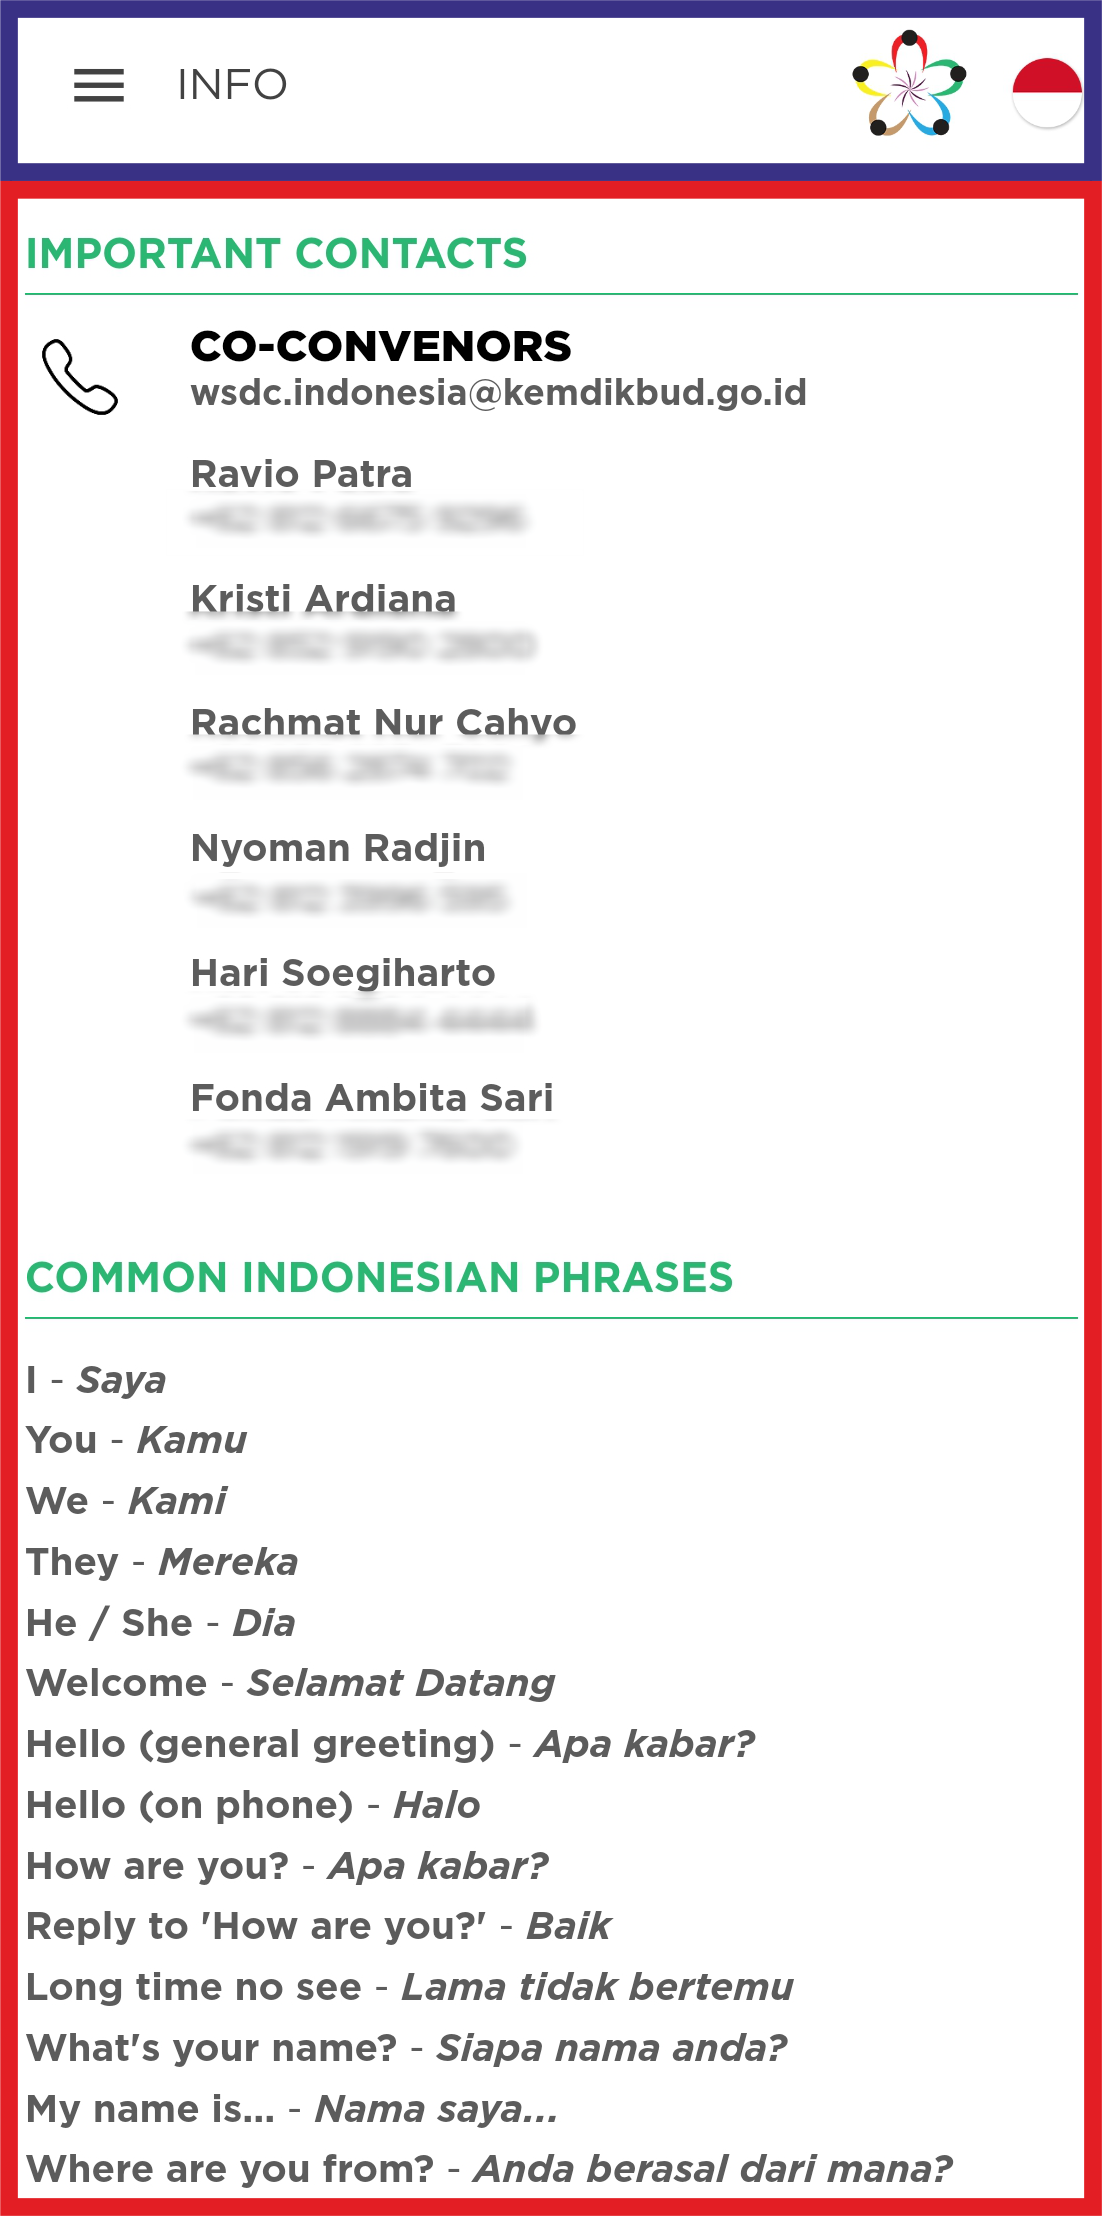
\includegraphics[scale=0.465]{Gambar/InfoPageWireframe.png}
         	\caption{Wireframe Komponen Info Aplikasi WSDC 2017 Bali terdahulu}
         	\label{fig:InfoPageWireframe}
     	\end{subfigure}
     	\hspace*{0.5in}
     	\begin{subfigure}[b]{0.43\textwidth}
         	\centering
         	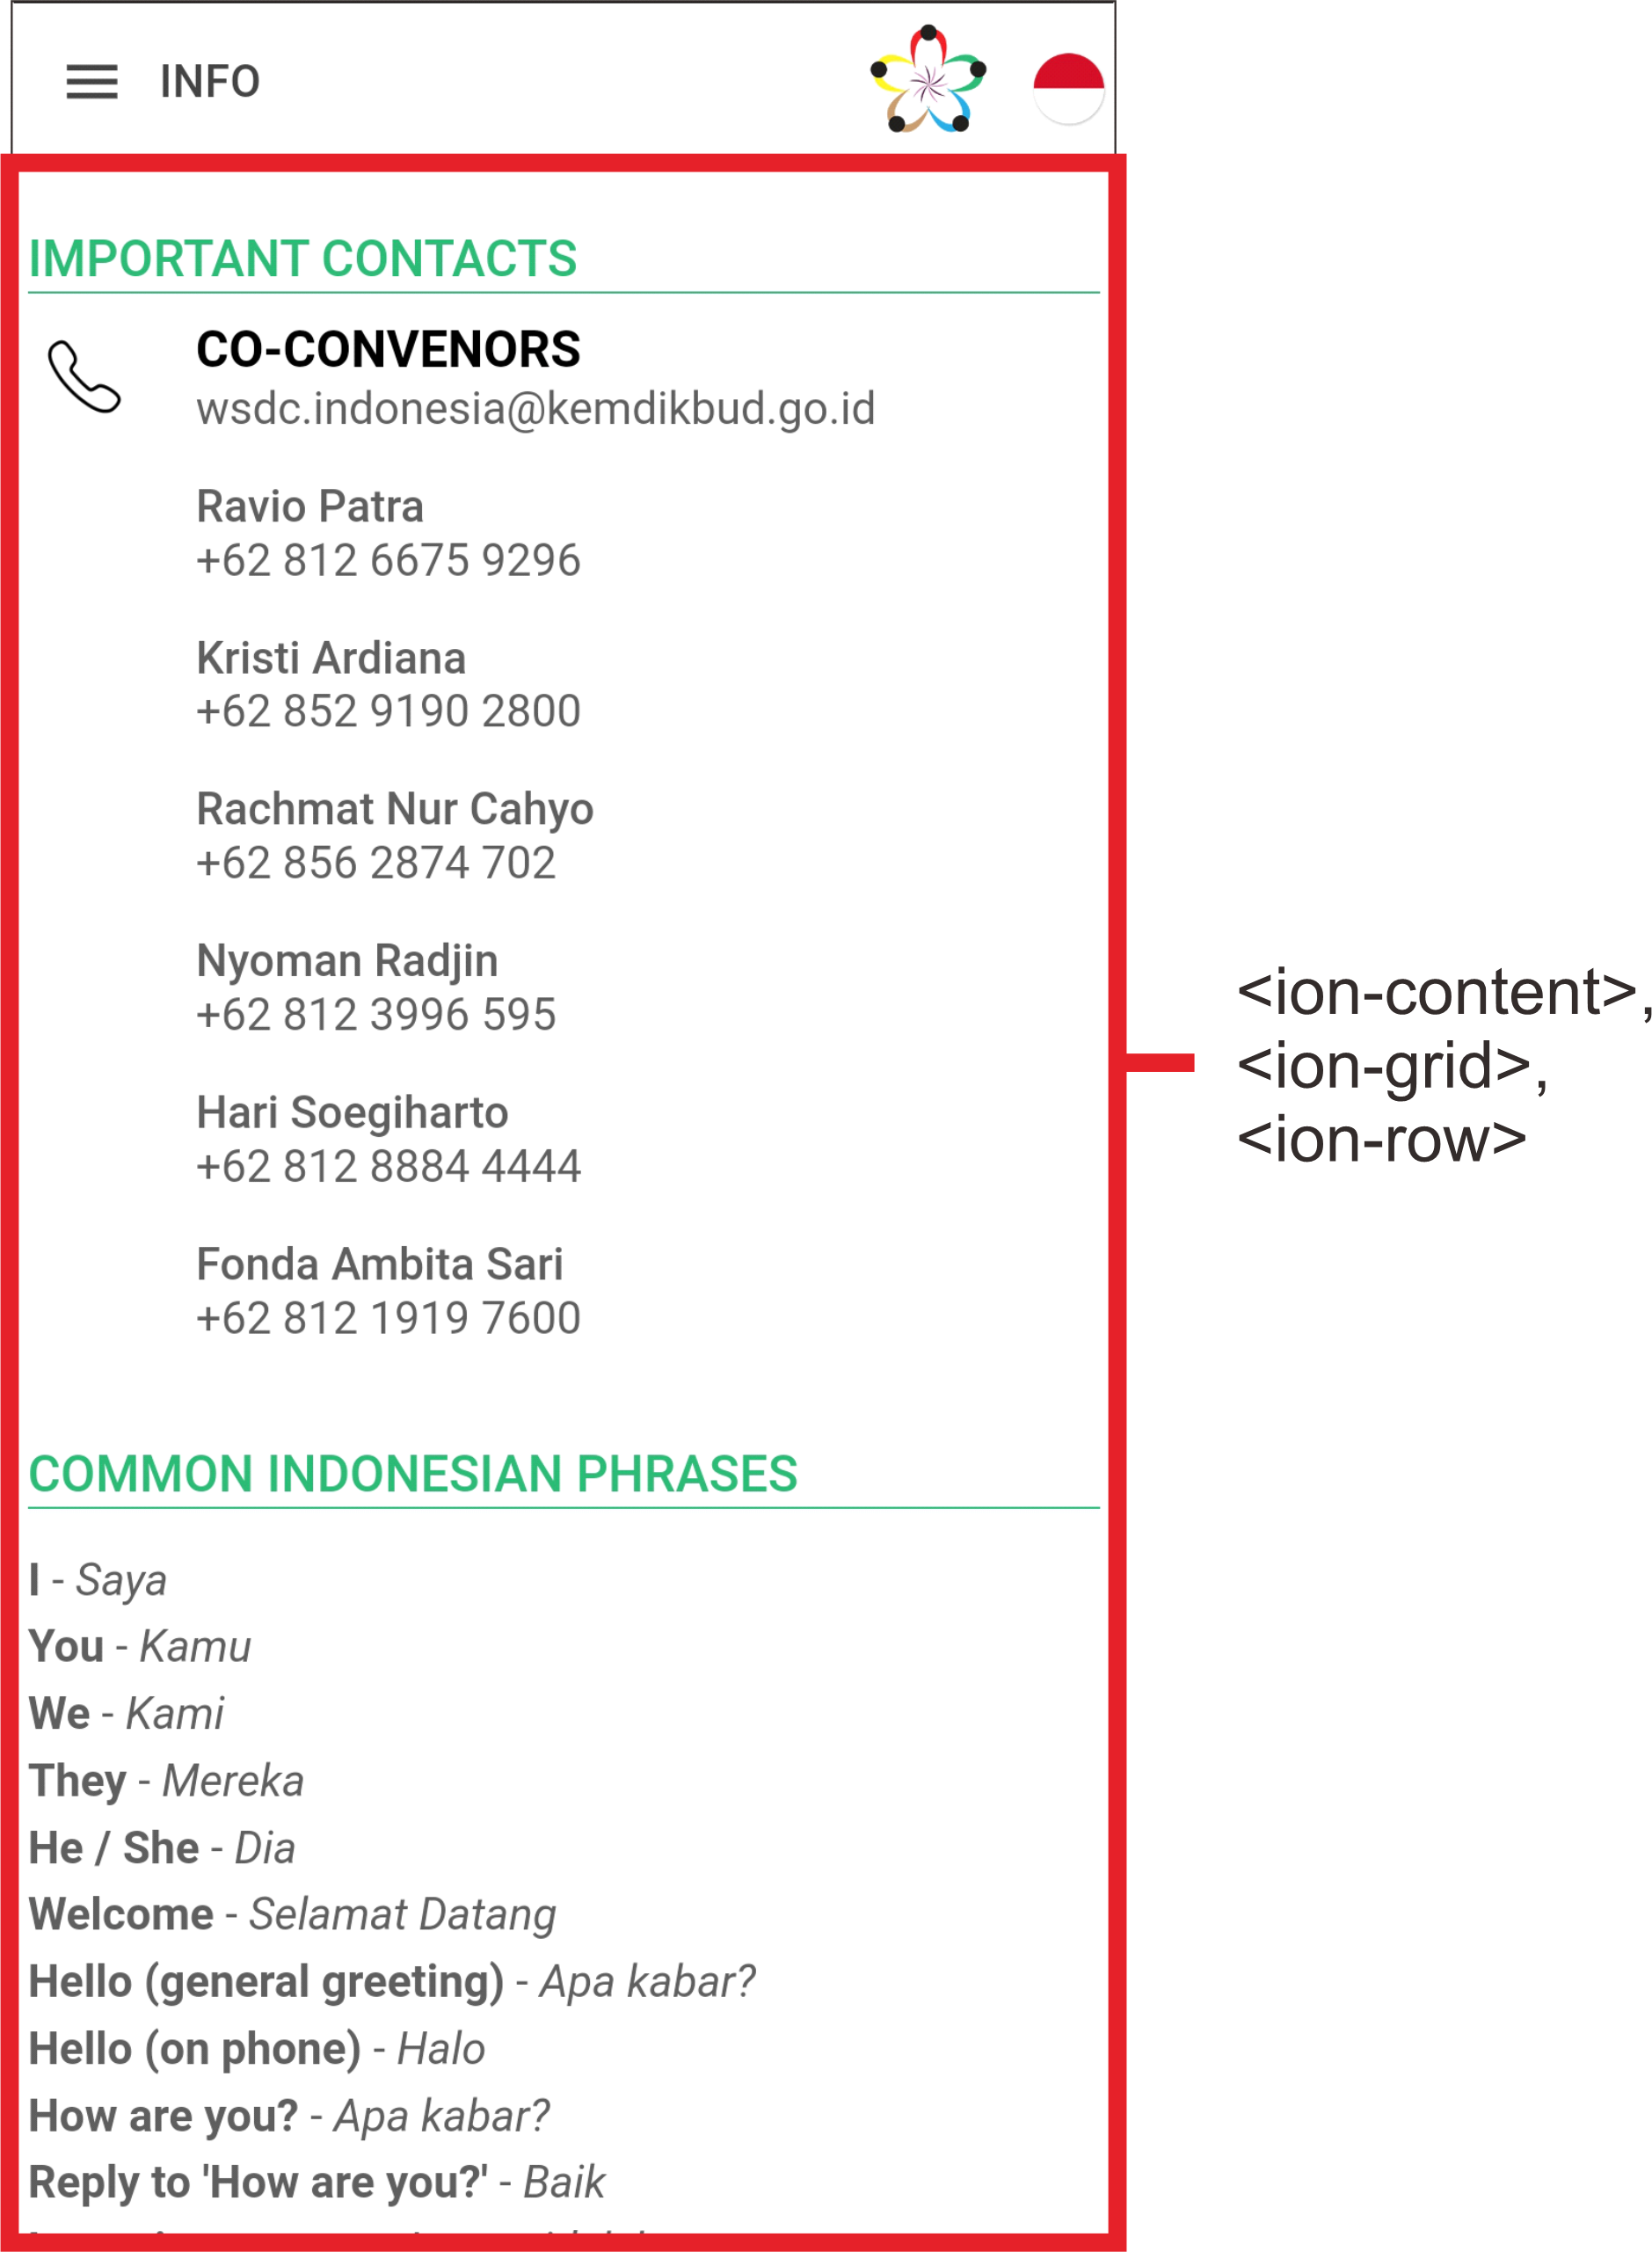
\includegraphics[scale=0.4]{Gambar/InfoPageKini.png}
         	\caption{UI Component Komponen Info Aplikasi WSDC 2017 Bali terbaru}
         	\label{fig:InfoPageKini}
     	\end{subfigure}
        \caption{Komponen Info pada Aplikasi WSDC 2017 Bali}
        \label{fig:UIComponent1}
	\end{figure}
	\begin{enumerate}
		\item Analisis pada Aplikasi WSDC 2017 Bali terdahulu \\
		Komponen ini memiliki sebuah \textit{file} TypeScript untuk mengatur keseluruhan halaman. Di dalam \textit{file} info.ts terdapat sebuah \textit{decorator} @Component untuk komponen (Kode~\ref{lst:componentinfo}). Di dalam decorator ini terdapat CSS \textit{selector} untuk memilih CSS yang akan digunakan, serta \textbf{templateUrl} untuk mendefinisikan ekxternal HTML \textit{template} yang akan digunakan. \textit{Template} HTML yang digunakan adalah \textit{file} info.html. 
	
\begin{lstlisting}[label={lst:componentinfo}, caption=@Component pada info.ts]
@Component({
  selector: 'page-info',
  templateUrl: 'info.html'
})
\end{lstlisting} 

	Terdapat kelas InfoPage pada komponen info. Kelas ini hanya berisi \textit{constructor} yang digunakan untuk menginisialisai halaman yang akan digunakan. \textit{Constructor} sendiri berfungsi untuk memuat data info dari penyimpanan dan memasukannya ke dalam sebuah variabel lokal.
	Terdapat \textit{file} info.html yang digunakan untuk menampilkan tata letak dari halaman info. Terdapat beberapa komponen yang disediakan oleh Ionic Framework, yang diimplementasikan ke dalam halaman info. Diantaranya adalah sebagai berikut:
	
	\begin{itemize}
		\item \textit{Header} \\
		Halaman info memiliki \textit{header} dengan \textit{tag} \texttt{<ion-header>} (Kode~\ref{lst:headerInfo}) seperti pada gambar~\ref{fig:InfoPageWireframe}. \textit{Tag} tersebut merupakan komponen \textit{parent} yang menampung komponen navbar yang ditandai dengan kotak berwarna biru. Di dalam navbar tersebut, terdapat sebuah \textit{tag} \texttt{<button>} untuk memunculkan \textit{sidemenu} dan \textit{tag} \texttt{<ion-icon>} untuk menampilkan icon dari tombol pada \textit{tag button}. Terdapat \textit{tag} \texttt{<ion-title>} sebagai judul dari halaman, yaitu ``Info''.
	
\begin{lstlisting}[label={lst:headerInfo}, caption=\textit{Header} pada info.html]
<ion-header>
  <ion-navbar>
    <button ion-button menuToggle>
      <ion-icon name="menu"></ion-icon>
    </button>
    <ion-title>Info</ion-title>
  </ion-navbar>
</ion-header>
\end{lstlisting} 

		\item \textit{Content} \\
		\textit{Content} pada halaman info memiliki \textit{tag} \texttt{<ion-content>} (Kode~\ref{lst:contentInfo}) yang pada gambar~\ref{fig:InfoPageWireframe} dengan kotak berwarna merah. Di dalam \textit{tag} info terdapat \textit{tag} \texttt{<ion-grid>} untuk mengatur \textit{layout} dari \textit{content}. Di dalam \textit{tag} \texttt{<ion-grid>} terdapat sebuah \textit{tag} \texttt{<ion-row>} yang berisi sebuah \textit{tag} \texttt{<div>}. \textit{Tag} tersebut berisi info yang di dapatkan pada \textit{constructor} di \textit{file} info.ts.

\begin{lstlisting}[label={lst:contentInfo}, caption=\textit{Content} pada info.html]
<ion-content>
  <ion-grid>
    <ion-row>
      <div [innerHTML]=wsdcInfoData>
      </div>
    </ion-row>
  </ion-grid>
</ion-content>
\end{lstlisting} 
	\end{itemize}
		\item Perancangan Aplikasi WSDC 2017 Bali terbaru \\
		Pada komponen info, terdapat beberapa UI Component yang akan diimplementasikan seperti pada gambar~\ref{fig:InfoPageKini}, diantaranya adalah sebagai berikut:
		\begin{itemize}
			\item Content \\
		Komponen ini akan digunakan sebagai penyedia area konten yang digunakan untuk mengontrol area yang dapat digulir dan menampilkan isi konten dari halaman info. UI Component \textit{Content} dengan \textit{tag} \texttt{<ion-content>} pada Ionic Framework versi 6 tidak mengalami perubahan dari Ionic Framework versi 3.
		
			\item \textit{Grid} \\
		Komponen ini akan digunakan untuk membangun tata letak kustom pada halaman info, yang terdiri dari baris. UI Component \textit{Grid} dengan \textit{tag} \texttt{<ion-grid>} dan \texttt{<ion-row>} pada Ionic Framework versi 6 tidak mengalami perubahan dari Ionic Framework versi 3
		\end{itemize}
	\end{enumerate}
	
	\item Komponen \textit{Result} \\
	Komponen \textit{Result} digunakan untuk melihat hasil dari pertandingan yang berisi pemenang dan skornya dari masing-masing babak pertandingan.
	\begin{figure}[H]
    	\centering
     	\begin{subfigure}[b]{0.43\textwidth}
        	\centering
         	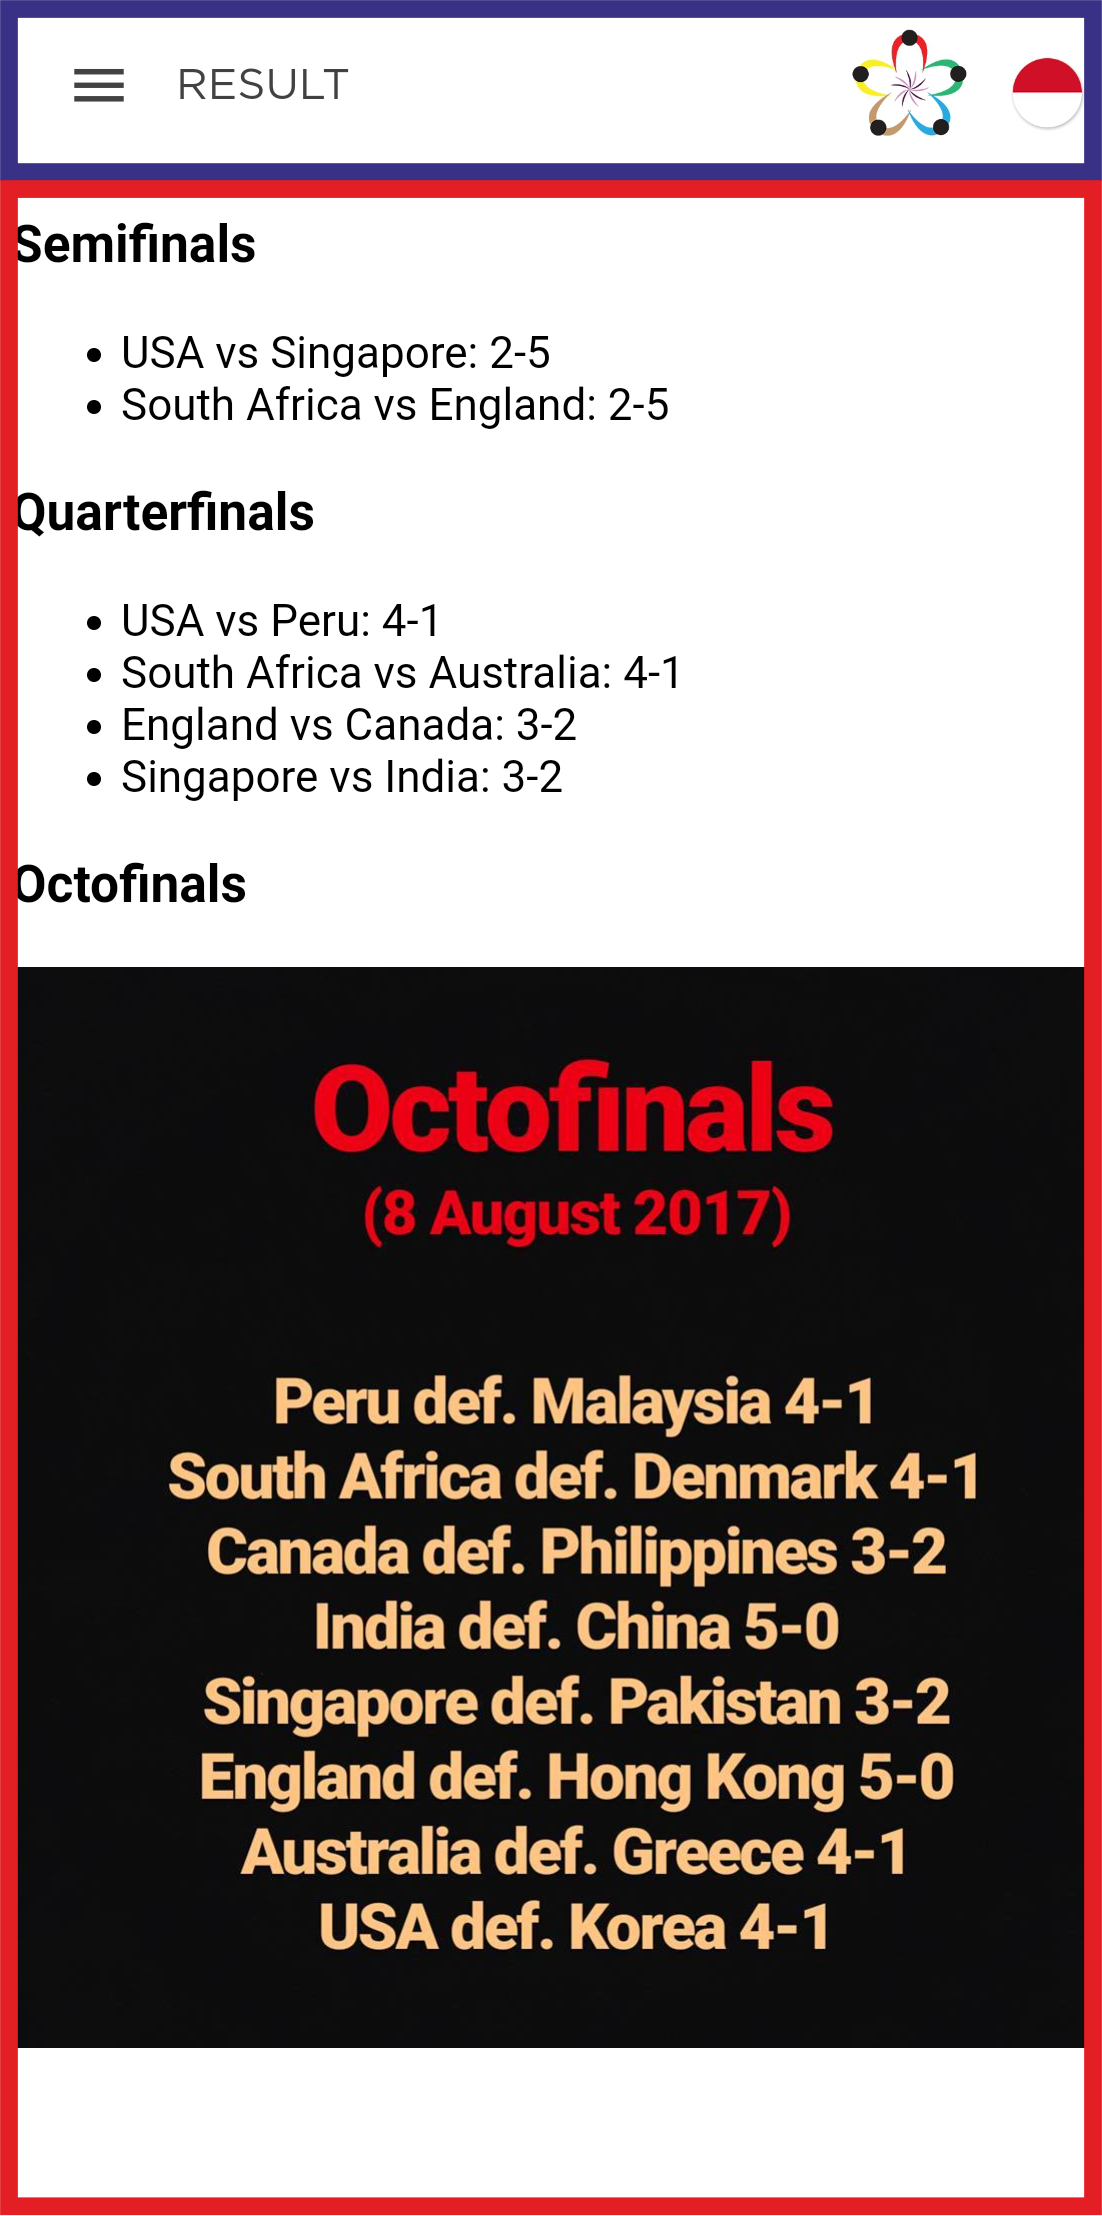
\includegraphics[scale=0.465]{Gambar/ResultPageWireframe.png}
         	\caption{Wireframe Komponen \textit{Result} Aplikasi WSDC 2017 Bali terdahulu}
         	\label{fig:ResultPageWireframe}
     	\end{subfigure}
     	\hspace*{0.5in}
     	\begin{subfigure}[b]{0.43\textwidth}
         	\centering
         	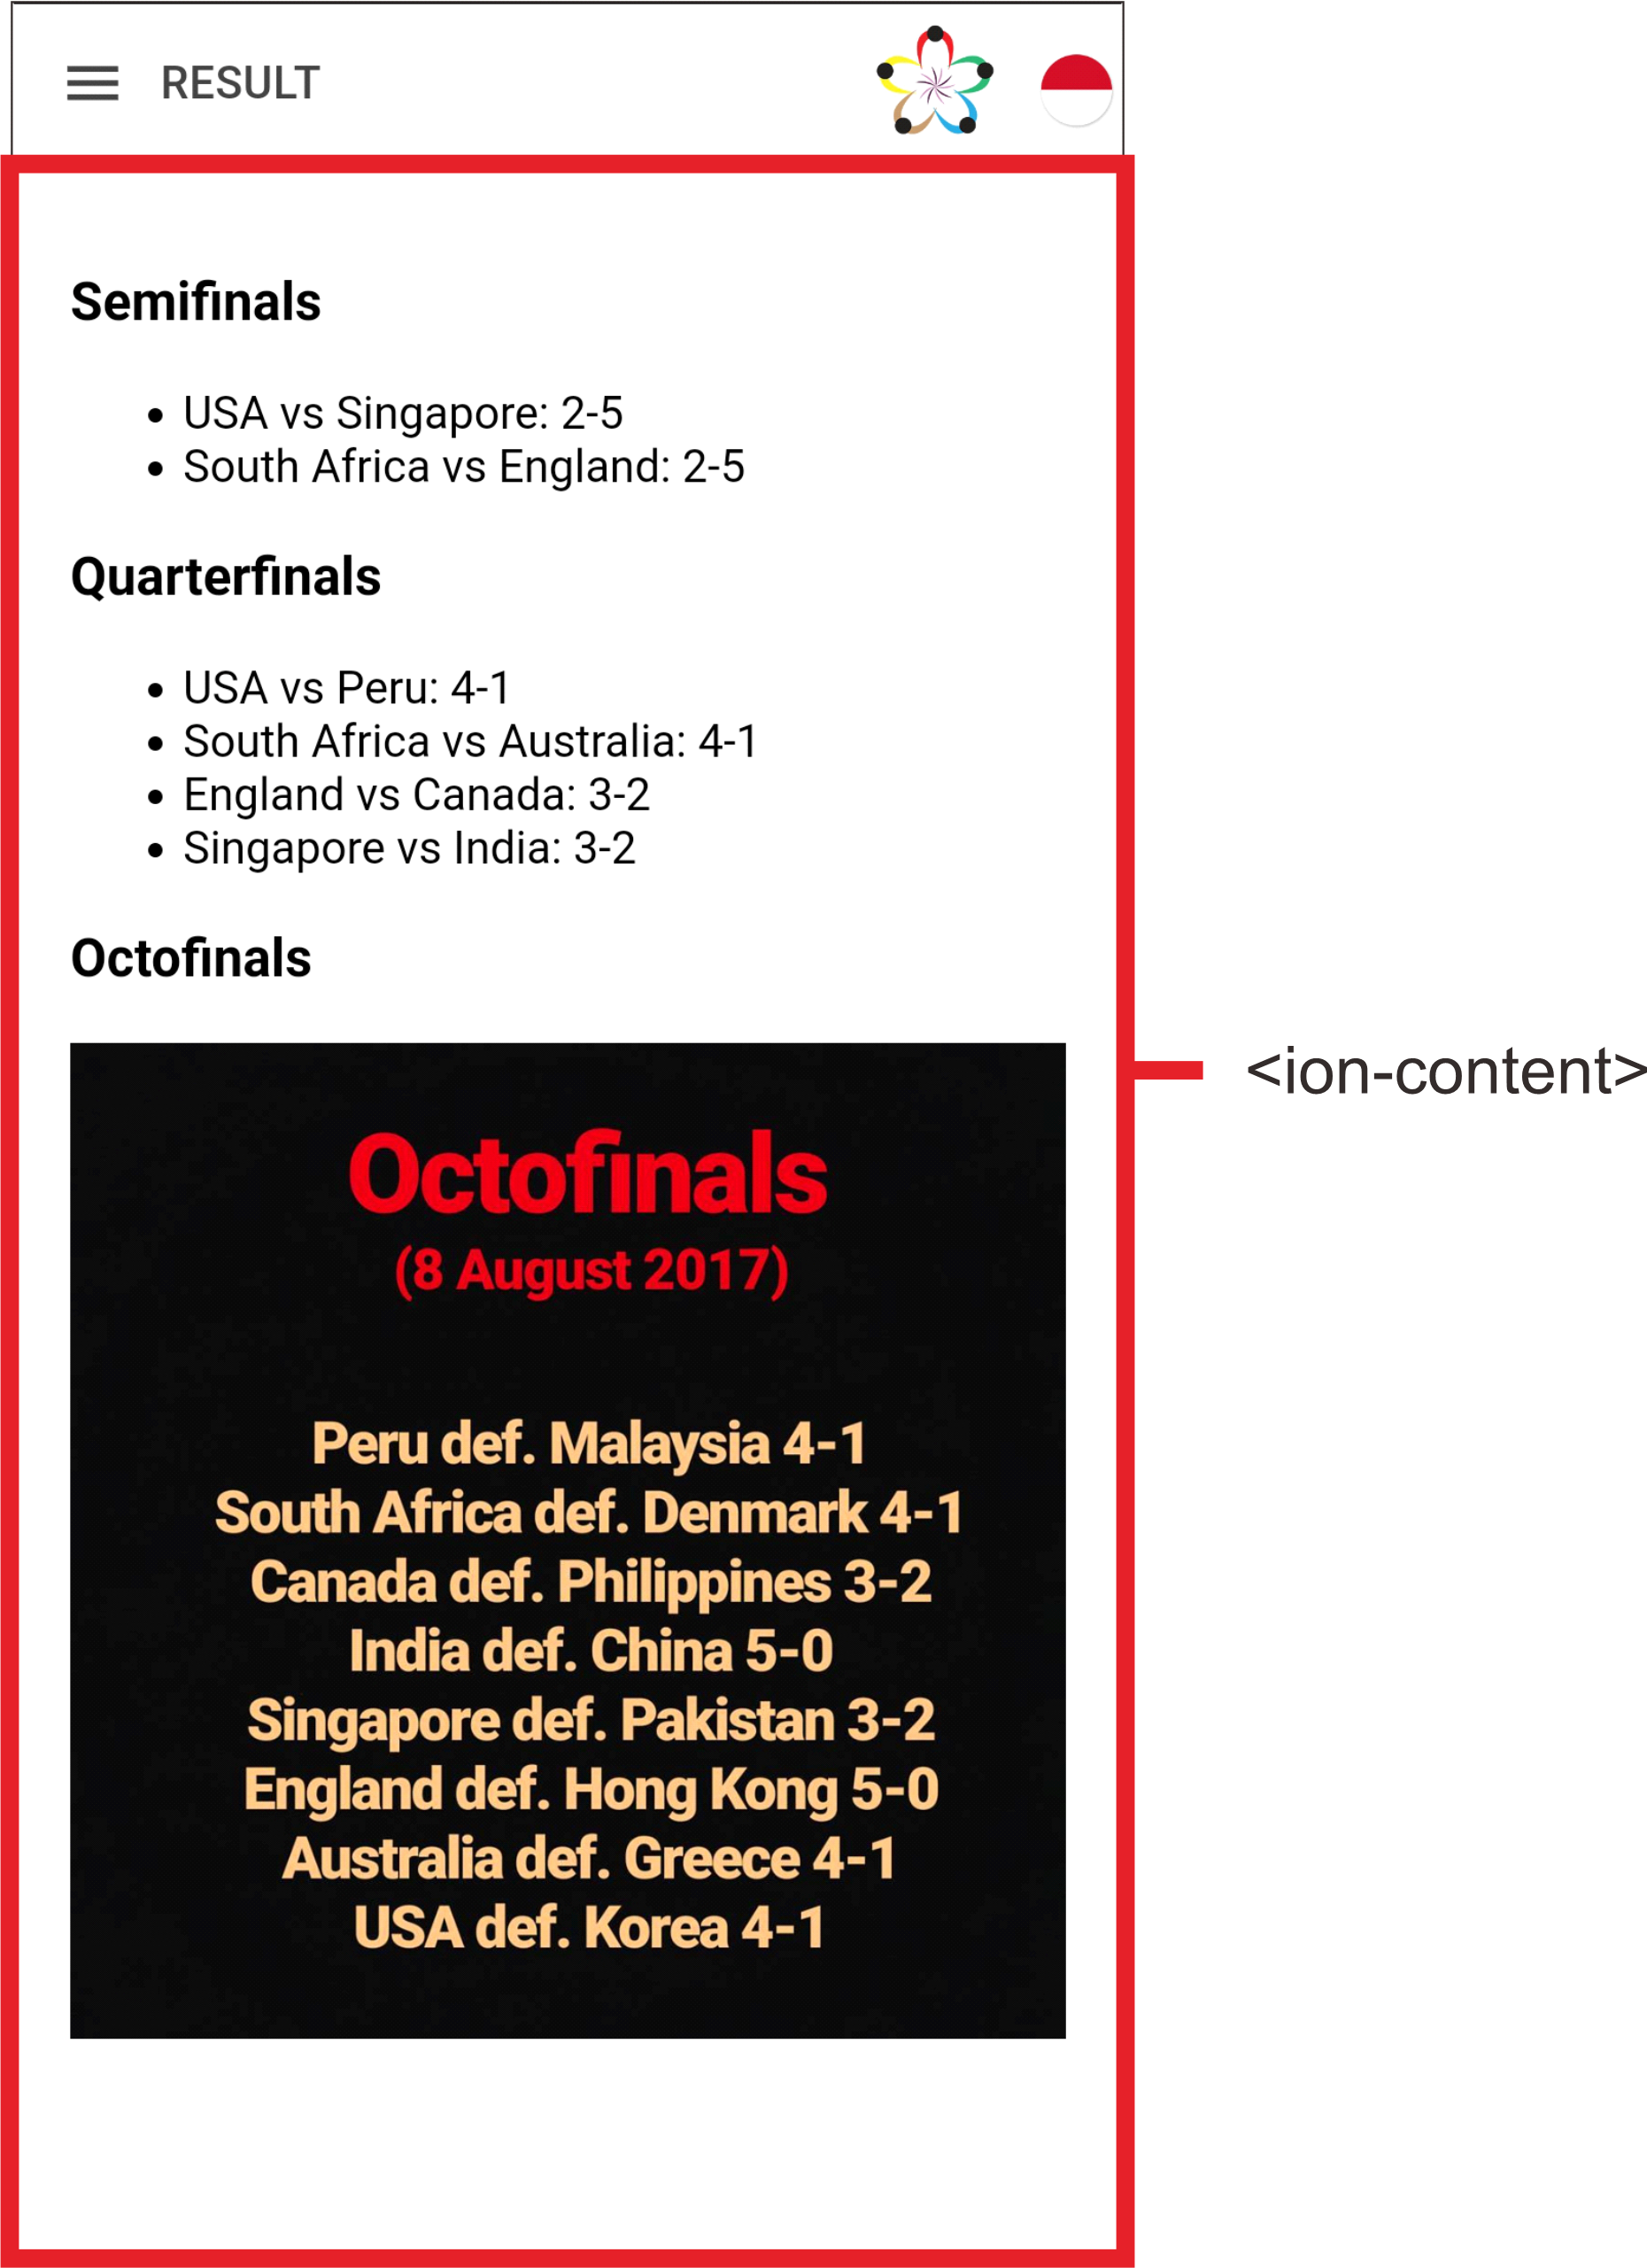
\includegraphics[scale=0.4]{Gambar/ResultPageKini.png}
         	\caption{UI Component Komponen \textit{Result} Aplikasi WSDC 2017 Bali terbaru}
         	\label{fig:ResultPageKini}
     	\end{subfigure}
        \caption{Komponen \textit{Result} pada Aplikasi WSDC 2017 Bali}
        \label{fig:UIComponent1}
	\end{figure}
	\begin{enumerate}
		\item Analisis pada Aplikasi WSDC 2017 Bali terdahulu \\
		Komponen ini memiliki sebuah \textit{file} TypeScript untuk mengatur keseluruhan halaman. Di dalam \textit{file} result.ts terdapat sebuah \textit{decorator} @Component untuk komponen (Kode~\ref{lst:componentresult}) dan \textit{decorator} @ViewChild (Kode~\ref{lst:viewchildtresult}). Di dalam decorator ini terdapat CSS \textit{selector} untuk memilih CSS yang akan digunakan, serta \textbf{templateUrl} untuk mendefinisikan ekxternal HTML \textit{template} yang akan digunakan. \textit{Template} HTML yang digunakan adalah \textit{file} info.html. @ViewChild digunakan untuk memanggil elemen dari DOM untuk memanggil komponen API ke dalam TypeScript, yaitu pada komponen \textit{result} adalah resultIFrame yang berada di \textit{file} result.html.
	
\begin{lstlisting}[ label={lst:componentresult}, caption=@Component pada result.ts]
@Component({
  selector: 'page-result',
  templateUrl: 'result.html'
})
\end{lstlisting} 

\begin{lstlisting}[label={lst:viewchildtresult}, caption=@ViewChild pada result.ts]
@ViewChild('resultIFrame') resultIFrame: ElementRef;
\end{lstlisting} 

	Terdapat kelas ResultPage dengan beberapa \textit{method} yang digunakan, yaitu:
	
	\begin{itemize}
		\item ionViewDidLoad() \\
		\textit{Method} ini merupakan sebuah \textit{lifecycle event} yang dijalankan saat halaman \textit{result} telah dimuat. \textit{Event} ini hanya berjalan satu kali, jadi jika sudah melakukan cache terhadap halaman ini, maka ionViewDidLoad() tidak akan berjalan lagi. \textit{Lifecycle event} ini berguna untuk melakukan pengaturan awal, yaitu untuk memuat data \textit{result} yang sudah disimpan di dalam penyimpanan internal. Setelah berhasil memuat data \textit{result}, data tersebut akan dimasukan ke dalam \textit{child} resultIFrame. Terakhir, akan dipanggil \textit{method} presentLoading().
		\item presentLoading() \\
		\textit{Method} ini berfungsi untuk menampilkan sebuah \textit{overlay} yang menunjukkan sebuah pesan dan indikator pemuatan saat pertama kali halaman \textit{draw} dimuat. Karena \textit{overlay} ini muncul di atas konten aplikasi, maka aktivitas pengguna akan diblokir untuk sementara sampai seluruh halaman dimuat, yaitu sampai \textit{method} onDrawIframeLoad() selesai. 
		\item onResultIframeLoad() \\
		\textit{Method} ini merupakan sebuah \textit{template statement} dipanggil oleh \textit{event} di dalam tag \texttt{<iframe>} pada result.html yaitu \textit{event} (load). \textit{Method} ini berfungsi untuk menampilkan data yang telah diambil yang disimpan di dalam \textit{child} resultIFrame.
	\end{itemize}
	
	Terdapat \textit{file} result.html yang digunakan untuk menampilkan tata letak dari halaman \textit{result}. Terdapat beberapa komponen yang disediakan oleh Ionic Framework, yang diimplementasikan ke dalam halaman \textit{result}. Diantaranya adalah sebagai berikut:
	
	\begin{itemize}
		\item \textit{Header} \\
		Halaman \textit{result} memiliki \textit{header} dengan \textit{tag} \texttt{<ion-header>} (Kode~\ref{lst:headerResult}) seperti pada gambar~\ref{fig:ResultPageWireframe}. \textit{Tag} tersebut merupakan komponen \textit{parent} yang menampung komponen navbar yang ditandai dengan kotak berwarna biru. Di dalam navbar tersebut, terdapat sebuah \textit{tag} \texttt{<button>} untuk memunculkan \textit{sidemenu}, dan \texttt{<ion-icon>} untuk menampilkan icon dari tombol pada \textit{tag button}. Terdapat \textit{tag} \texttt{<ion-title>} sebagai judul dari halaman, yaitu ``Result''.

\begin{lstlisting}[label={lst:headerResult}, caption=\textit{Header} pada result.html]
<ion-header>
  <ion-navbar>
    <button ion-button menuToggle>
      <ion-icon name="menu"></ion-icon>
    </button>
    <ion-title>Result</ion-title>
  </ion-navbar>
</ion-header>
\end{lstlisting}

		\item \textit{Content}\\
		\textit{Content} pada halaman result memiliki \textit{tag} \texttt{<ion-content>} (Kode~\ref{lst:contentResult}) yang pada gambar~\ref{fig:ResultPageWireframe} dengan kotak berwarna merah. Di dalam \textit{tag} \texttt{<ion-content>} terdapat \textit{tag} \texttt{<iframe>}. \textit{Tag} tersebut berisi informasi mengenai daftar pemenang acara WSDC 2017 bali yang di dapatkan pada \textit{method} onResultIframeLoad() di kelas ResultPage pada \textit{file} result.ts.
		
\begin{lstlisting}[label={lst:contentResult}, caption=\textit{Content} pada result.html]
<ion-content>
  <iframe #resultIFrame (load)="onResultIframeLoad()" class="iframe-fullscreen"></iframe>
</ion-content>
\end{lstlisting} 
	\end{itemize}
	\newpage
		\item Perancangan Aplikasi WSDC 2017 Bali terbaru \\
		Pada komponen \textit{Result}, terdapat sebuah UI Component, yaitu \textit{Content} seperti pada gambar~\ref{fig:ResultPageKini}. Komponen \textit{content} akan digunakan sebagai penyedia area konten yang digunakan untuk mengontrol area konten dan menampilkan isi konten dari halaman \textit{result}. UI Component \textit{Content} dengan \textit{tag} \texttt{<ion-content>} pada Ionic Framework versi~6~tidak~mengalami perubahan~dari~Ionic~Framework~versi~3. 
	\end{enumerate}
	
	\item Komponen \textit{Schedule} \\
	Komponen \textit{Schedule} digunakan untuk melihat jadwal pertandingan yang berisi waktu, tanggal, hari, dan lokasi untuk setiap jadwal pertandingan WSDC 2017 Bali.
	\begin{figure}[H]
    	\centering
     	\begin{subfigure}[b]{0.43\textwidth}
        	\centering
         	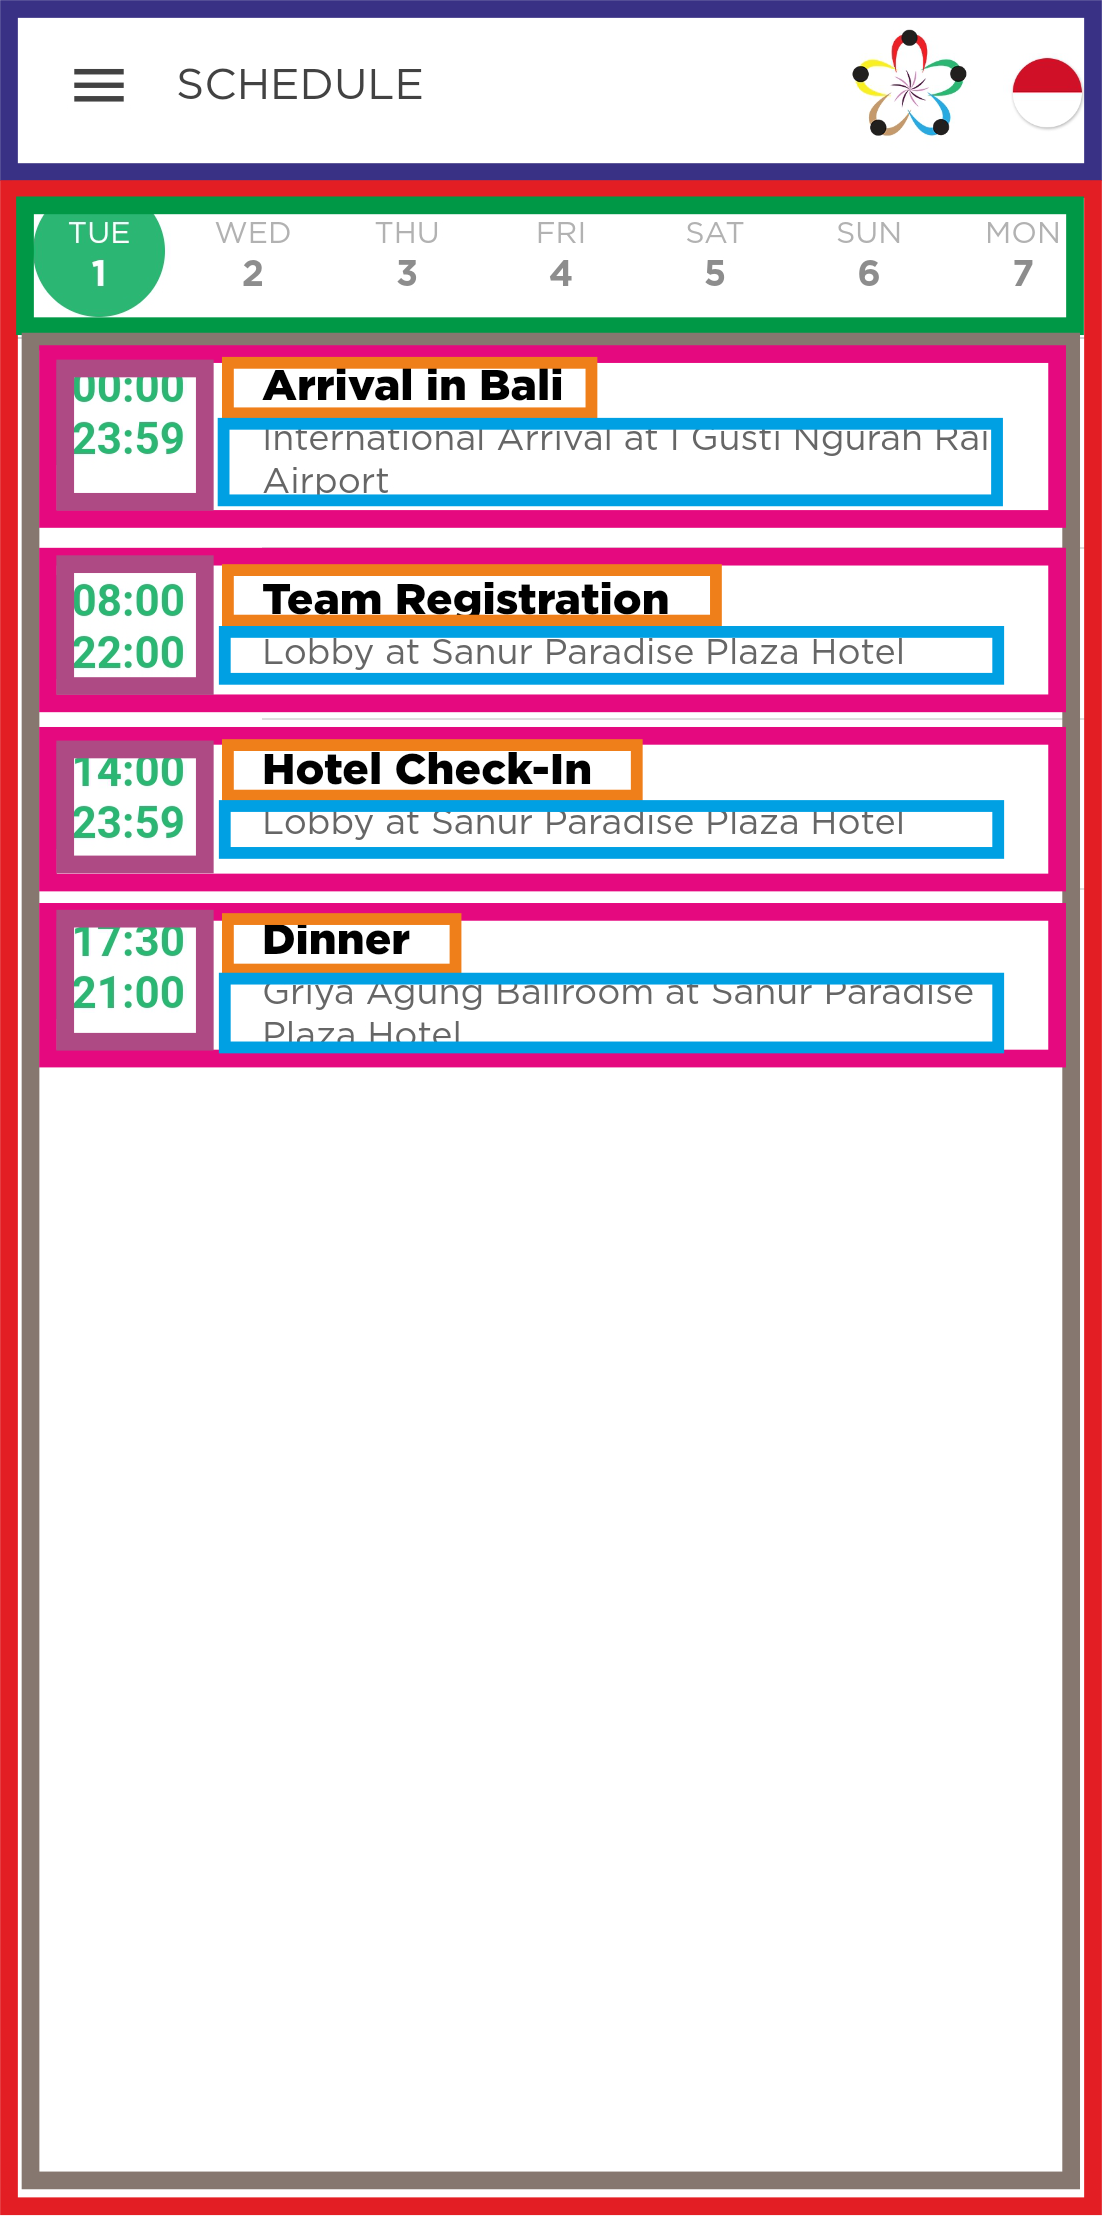
\includegraphics[scale=0.465]{Gambar/SchedulePageWireframe.png}
         	\caption{Wireframe Komponen \textit{Schedule} Aplikasi WSDC 2017 Bali terdahulu}
         	\label{fig:SchedulePageWireframe}
     	\end{subfigure}
     	\hspace*{0.5in}
     	\begin{subfigure}[b]{0.43\textwidth}
         	\centering
         	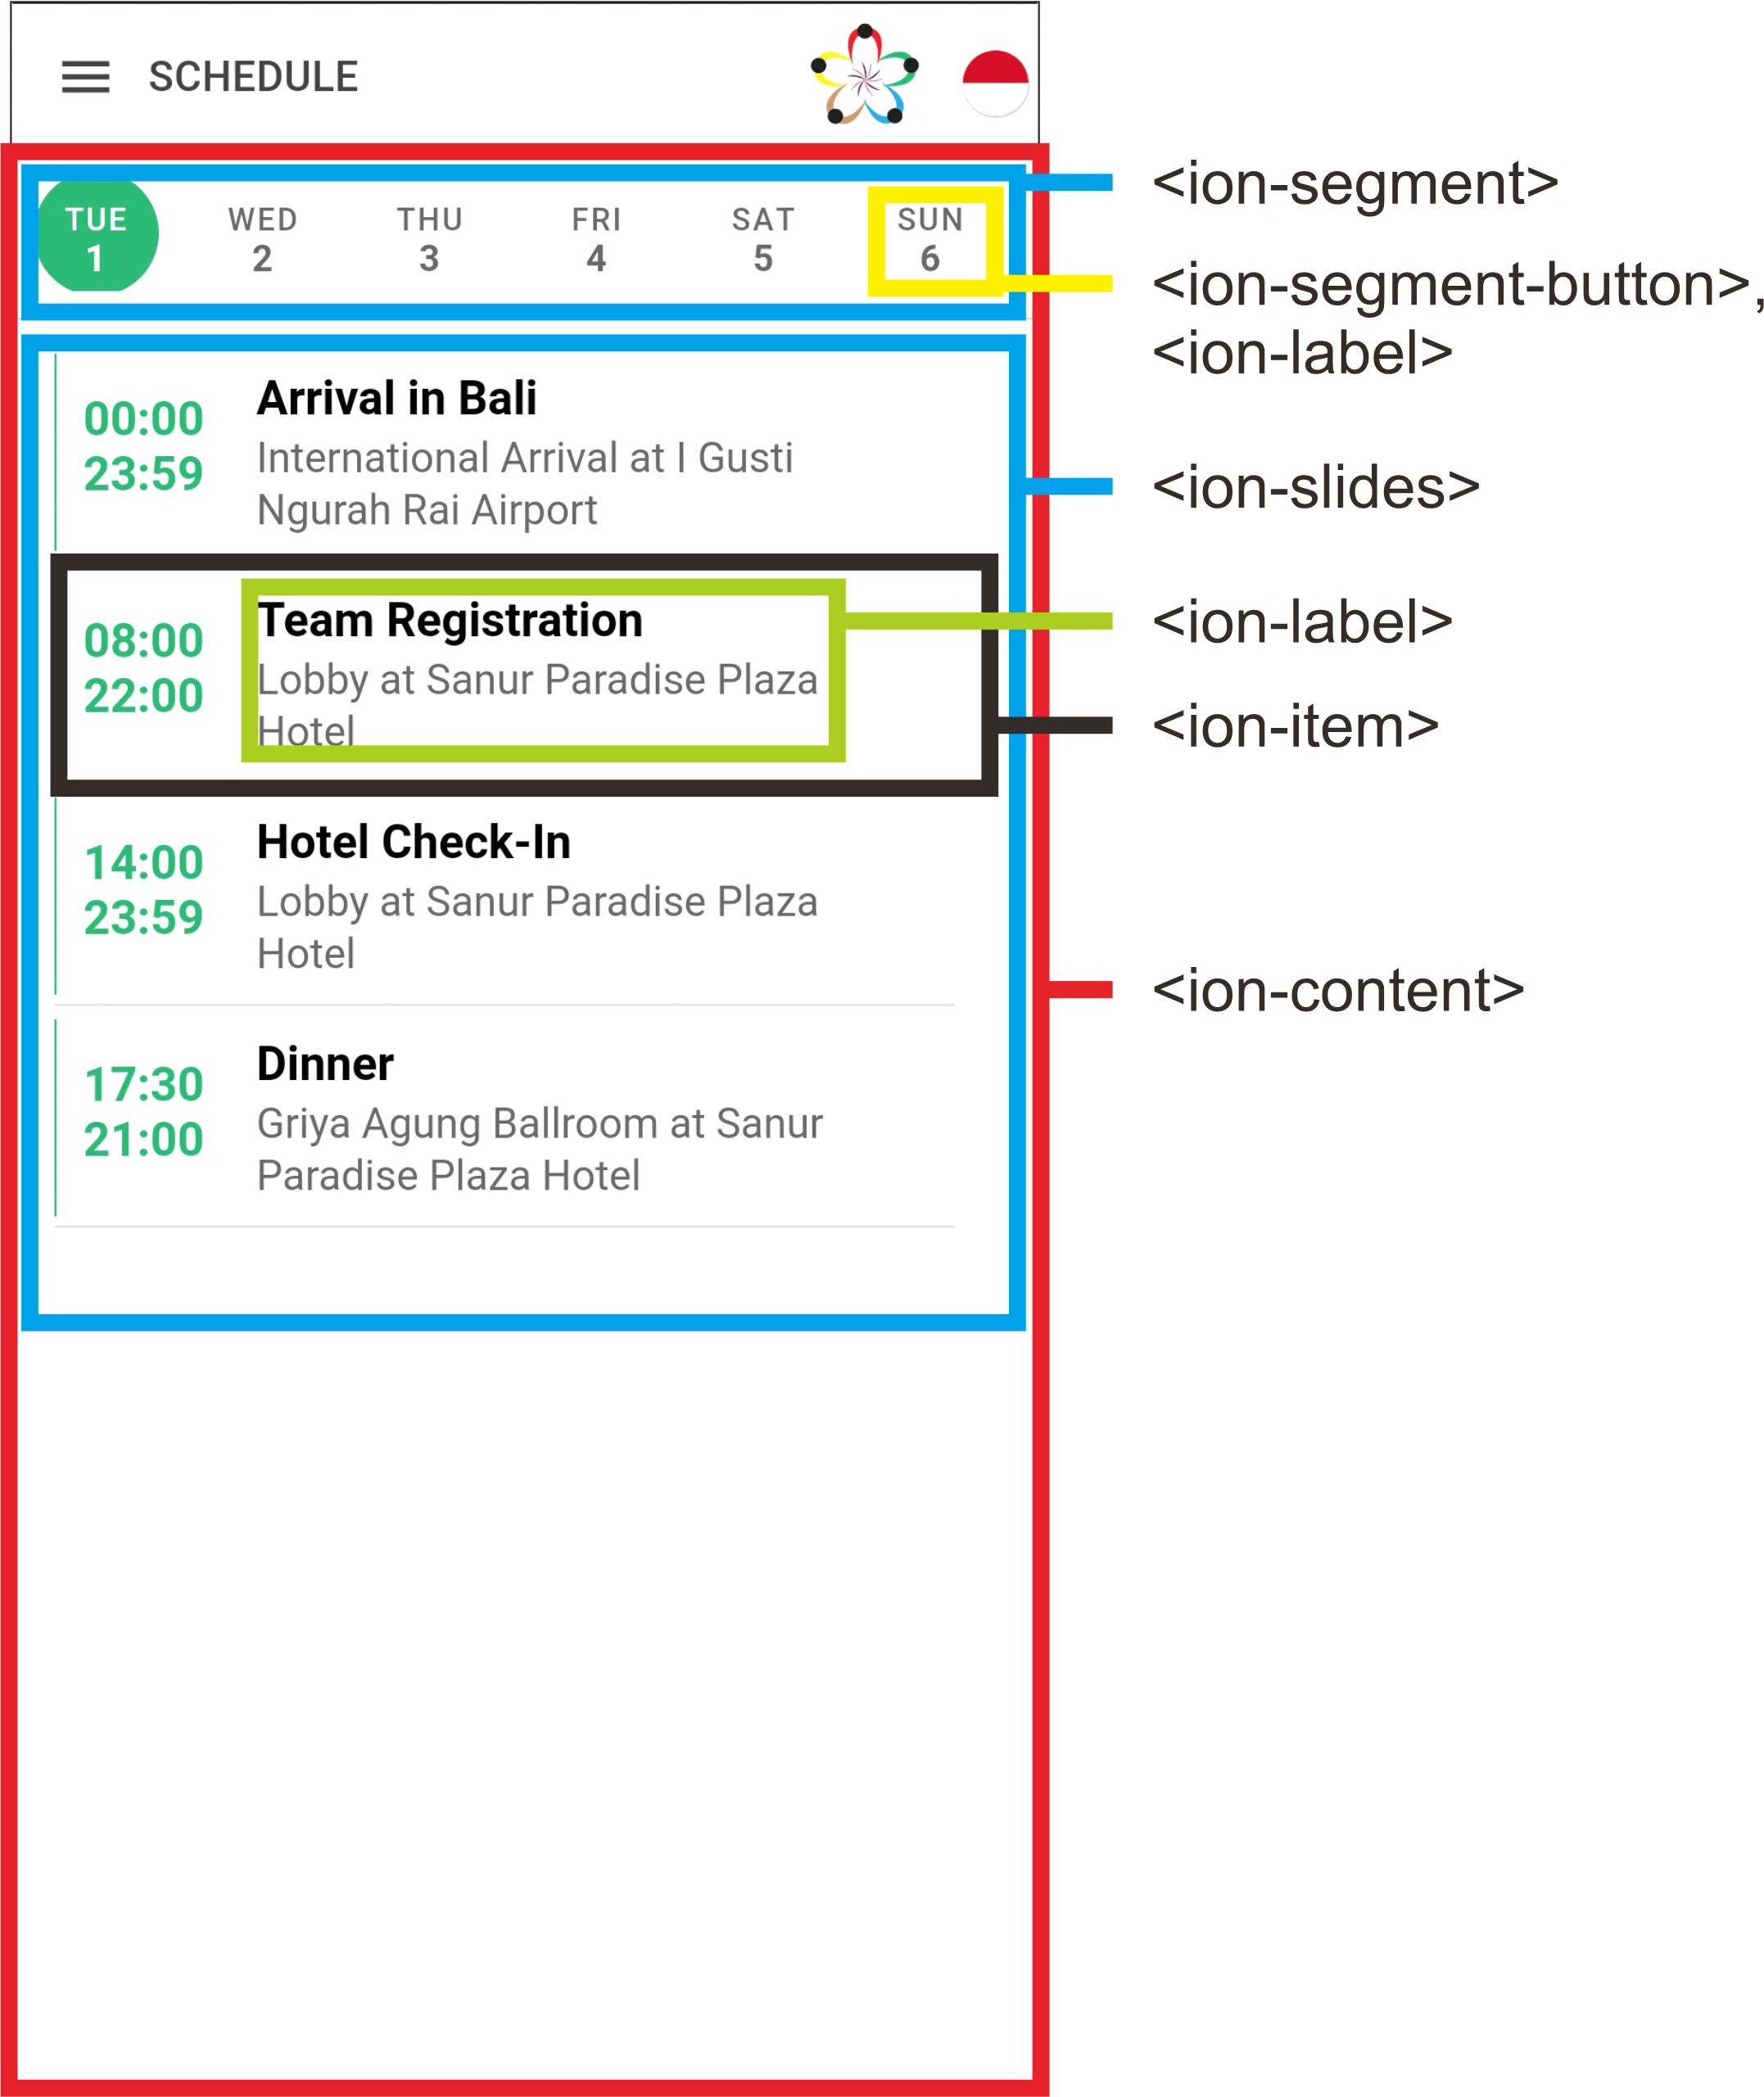
\includegraphics[scale=0.4]{Gambar/SchedulePageKini.png}
         	\caption{UI Component Komponen \textit{Schedule} Aplikasi WSDC 2017 Bali terbaru}
         	\label{fig:SchedulePageKini}
     	\end{subfigure}
        \caption{Komponen \textit{Schedule} pada Aplikasi WSDC 2017 Bali}
        \label{fig:UIComponent1}
	\end{figure}
	\begin{enumerate}
		\item Analisis pada Aplikasi WSDC 2017 Bali terdahulu \\
		Komponen ini memiliki sebuah \textit{file} TypeScript untuk mengatur keseluruhan halaman. Di dalam \textit{file} schedule.ts terdapat sebuah \textit{decorator} @Component untuk komponen (Kode~\ref{lst:componentschedule}) dan dua \textit{decorator} @ViewChild (Kode~\ref{lst:viewchildtresult}). Di dalam decorator ini terdapat CSS \textit{selector} untuk memilih CSS yang akan digunakan, serta \textbf{templateUrl} untuk mendefinisikan ekxternal HTML \textit{template} yang akan digunakan. \textit{Template} HTML yang digunakan adalah \textit{file} info.html. @ViewChild digunakan untuk memanggil elemen dari DOM untuk memanggil komponen API ke dalam TypeScript, yaitu pada komponen \textit{result} adalah scheduleSlider dan segmentContainer yang berada di \textit{file} result.html. scheduleSlider berfungsi untuk menyimpan konten dari sebuah \textit{slide}. Sedangkan segmentContainer berfungsi untuk menyimpan konten dari sebuah \textit{segment}.
	\newpage
\begin{lstlisting}[label={lst:componentschedule}, caption=@Component pada schedule.ts]
@Component({
  selector: 'page-schedule',
  templateUrl: 'schedule.html'
})
\end{lstlisting}

\begin{lstlisting}[label={lst:viewchildtresult}, caption=@ViewChild pada schedule.ts]
@ViewChild('scheduleSlider') slider: Slides;
@ViewChild('segmentContainer') segmentContainer: ElementRef;
\end{lstlisting} 

	Terdapat kelas SchedulePage pada schedule.ts yang ini memiliki satu \textit{constructor}. \textit{Constructor} kelas ini berfungsi untuk mengambil data \textit{result} yang berada di dalam penyimpanan internal. Data tersebut kemudian disimpan ke dalam variabel lokal schedules. Kemudian akan mengatur \textit{segment} yang aktif pada saat pertama kali halaman \textit{result} dibuka, yaitu \textit{segment} yang pertama dan menampilkan \textit{slide} pertama yang berisi jadwal pada hari pertama. Terdapat beberapa \textit{method} yang digunakan, yaitu:
	
	\begin{itemize}
		\item onSegmentChanged(segmentButton) \\
		\textit{Method} ini merupakan sebuah \textit{template statement} dipanggil oleh \textit{event} di dalam tag \texttt{<ion-segment>} pada schedule.html yaitu \textit{event} (ionChange). (ionChange) merupakan \textit{event} yang dimiliki oleh UI Component ion-segment milik Ionic Framework. \textit{Method} ini digunakan ketika pengguna memilih \textit{segment} pada \textit{tag} \texttt{<ion-segment>} di dalam \textit{file} schedule.html. \textit{Method} ini memiliki sebuah parameter segmentButton yang berisi \textit{event} dari sebuah segment. \textit{Child component} slides kemudian akan diubah sesuai dengan \textit{value} yang ada pada parameter, yaitu hari yang sedang aktif. 

		\item onSlideChanged() \\
		\textit{Method} ini merupakan sebuah \textit{template statement} dipanggil oleh \textit{event} di dalam \textit{tag} \texttt{<ion-slides>} pada schedule.html yaitu \textit{event} (ionSlideDidChange). (ionSlideDidChange) merupakan \textit{event} yang dimiliki oleh UI Component ion-slides milik Ionic Framework. \textit{Method} ini berfungsi untuk berpindah antar \textit{slides} saat pengguna menggeser \textit{slides} tersebut ke kanan atau ke kiri layar.
		\item getDayName(sqlDate: string) \\
		\textit{Method} ini berfungsi untuk mengembalikan nama hari dari parameter.
		\item getDate(sqlDate: string) \\
		\textit{Method} ini bergunsi untuk mengembalikan tanggal dari parameter.
	\end{itemize}
	
	Terdapat \textit{file} schedule.html yang digunakan untuk menampilkan halaman \textit{schedule}. Terdapat beberapa komponen yang disediakan oleh Ionic Framework, yang diimplementasikan ke dalam halaman \textit{schedule}. Diantaranya adalah sebagai berikut:
	
	\begin{itemize}
		\item \textit{Header} \\
		Halaman \textit{schedule} memiliki \textit{header} dengan \textit{tag} \texttt{<ion-header>} (Kode~\ref{lst:headerSchedule}) seperti pada gambar~\ref{fig:SchedulePageWireframe}. \textit{Tag} tersebut merupakan komponen \textit{parent} yang menampung komponen navbar yang ditandai dengan kotak berwarna biru. Di dalam navbar tersebut, terdapat sebuah \textit{tag} \texttt{<button>} untuk memunculkan \textit{sidemenu} dan \texttt{ion-icon>} untuk menampilkan icon dari tombol pada \textit{tag button}. Terdapat \textit{tag} \texttt{<ion-title>} sebagai judul dari halaman, yaitu ``Schedule''.
		
\begin{lstlisting}[label={lst:headerSchedule}, caption=\textit{Header} pada schedule.html]
<ion-header>
  <ion-navbar>
    <button ion-button menuToggle>
      <ion-icon name="menu"></ion-icon>
    </button>
    <ion-title>Schedule</ion-title>
  </ion-navbar>
</ion-header>
\end{lstlisting} 

		\item \textit{Content} \\
		\textit{Content} pada halaman result memiliki \textit{tag} \texttt{<ion-content>} (Kode~\ref{lst:contentSchedule}) yang pada gambar~\ref{fig:SchedulePageWireframe} dengan kotak berwarna merah. Di dalam \textit{tag} \texttt{<ion-content>} terdapat dua buah \textit{tag} \texttt{<div>} yang masing masing berisi \textit{tag} \texttt{<ion-segment>} dan \textit{tag} \texttt{<ion-slides>}. \textit{Tag} \texttt{<ion-segment>} digunakan untuk tampilan hari, seperti pada gambar~\ref{fig:SchedulePageWireframe} yang ditandai dengan kotak berwarna hijau. \textit{Tag} \texttt{<ion-slides>} digunakan untuk tampilan jadwal di dalam satu hari, seperti yang ditandai dengan kotak berwarna coklat. 
		
		Setiap jadwal yang berada di \textit{tag} \texttt{<ion-slides>} dibungkus dengan \textit{tag} \texttt{<ion-list>} seperti pada kotak berwarna merah muda di gambar~\ref{fig:SchedulePageWireframe}. Dalam satu \textit{tag} \texttt{<ion-list>} terdapat \textit{tag} \texttt{<ion-note>} yang berisi waktu mulai dan waktu selesai dari satu jadwal seperti yang ditandai dengan kotak berwarna ungu, \textit{tag} \texttt{<h3>} berisi nama acara seperti yang ditandai dengan kotak berwarna oranye, dan \textit{tag} \texttt{<p>} yang berisi tempat acara tersebut diadakan ditandai dengan kotak berwarna biru muda.



\begin{lstlisting}[label={lst:contentSchedule}, caption=\textit{Content} pada schedule.html]
<ion-content>
  <div id="schedulesContainer">
    <div id="schedulesSegments">
      <ion-segment #segmentContainer *ngIf="schedules" [(ngModel)]="selectedSegmentIdx" (ionChange)="onSegmentChanged($event)">
        <ion-segment-button *ngFor="let schedule of schedules; let i = index" [value]="i">
          <div class="day">{{getDayName(schedule.date)}}</div>
          <div class="date">{{getDate(schedule.date)}}</div>
        </ion-segment-button>
      </ion-segment>
    </div>
    <div id="schedulesSlides">
      <ion-slides #scheduleSlider (ionSlideDidChange)="onSlideChanged()">
        <ion-slide *ngFor="let schedule of schedules">
          <ion-list>
            <ion-item text-wrap *ngFor="let agenda of schedule.agenda">
              <ion-note item-start>
                {{agenda.start}}<br/>
                {{agenda.end}}
              </ion-note>
              <h3>{{agenda.title}}</h3>
              <p>{{agenda.subtitle}}</p>
            </ion-item>
          </ion-list>
        </ion-slide>
      </ion-slides>
    </div>
  </div>
</ion-content>
\end{lstlisting} 
		\item Perancangan Aplikasi WSDC 2017 Bali terbaru \\
		Pada komponen \textit{schedule}, terdapat beberapa UI Component yang akan diimplementasikan seperti pada gambar~\ref{fig:SchedulePageKini}, diantaranya adalah sebagai berikut:
		\begin{itemize}
			\item \textit{Content} \\
		Komponen ini akan digunakan sebagai penyedia area konten yang digunakan untuk mengontrol area yang dapat digulir dan menampilkan isi konten dari halaman \textit{schedule}. UI Component \textit{Content} dengan \textit{tag} \texttt{<ion-content>} pada Ionic Framework versi 6 tidak mengalami perubahan dari Ionic Framework versi 3.
		
			\item \textit{Item} \\
			\textit{Item} dengan \textit{tag} \texttt{<ion-item>} sejak Ionic 4 mengalami perubahan dibandingkan pada Ionic 3, yaitu wajib menambahkan \textit{label} dengan \textit{tag} \texttt{<ion-label>}. Pada aplikasi WSDC 2017 Bali saat ini yang menggunakan Ionic 3, tidak terdapat \textit{tag} \texttt{<ion-label>} pada \texttt{<ion-item>} (Kode~\ref{lst:itemScheduleWSDCOld}). Sedangkan sesuai dengan ketentuan yang berlaku, pada aplikasi yang akan dibangun yang menggunakan Ionic 6, akan menggunakan \textit{tag} \texttt{<ion-label>} di dalam \texttt{<ion-item>} (Kode~\ref{lst:itemScheduleWSDCNew}).
			
\begin{lstlisting}[label={lst:itemScheduleWSDCOld}, caption=\textit{Tag} <ion-item> dengan Ionic 3 di Aplikasi WSDC 2017 Bali Saat Ini]
<ion-item text-wrap *ngFor="let agenda of schedule.agenda">
	<ion-note item-start>
		{{agenda.start}}<br/>
        {{agenda.end}}
   </ion-note>
   <h3>{{agenda.title}}</h3>
   <p>{{agenda.subtitle}}</p>
</ion-item>
\end{lstlisting}

\begin{lstlisting}[label={lst:itemScheduleWSDCNew}, caption=\textit{Tag} <ion-item> dengan Ionic 6 di Aplikasi WSDC 2017 Bali yang Akan dibuat]
<ion-item *ngFor="let agenda of schedule.agenda;" >
	<ion-note item-start>
    	{{agenda.start}}<br/> 
        {{agenda.end}}
   	</ion-note>
    <ion-label class="ion-text-wrap">
    	<h3>{{agenda.title}}</h3>
        <p>{{agenda.subtitle}}</p>
    </ion-label>
</ion-item>
\end{lstlisting}
			\newpage
			\item \textit{List} \\
			\textit{List} berfungsi untuk menyimpan konten yang terdiri dari beberapa baris. \textit{List} dengan \textit{tag} \texttt{<ion-list>} akan terdiri dari beberapa baris item \texttt{<ion-item>} dan akan memiliki sebuah \textit{header}. UI Component \textit{List} dengan \textit{tag} \texttt{<ion-list>}, dan \texttt{<ion-item>} pada Ionic Framework versi 6 tidak mengalami perubahan dari Ionic Framework versi 3.	
		
			\item \textit{Segment} \\
		Komponen ini akan digunakan untuk pengguna agar dapat berpindah tampilan di dalam halaman yang sama. Seperti pada tampilan halaman jadwal yang ada pada aplikasi WSDC 2017 Bali saat ini, dimana pengguna dapat berpindah hari untuk mengetahui jadwal kegiatan pada hari tertentu yang dipilih oleh pengguna, namun masih berada di halaman yang sama, yaitu halaman Schedule. UI Component \textit{Segment} dengan \textit{tag} \texttt{<ion-segment>} pada Ionic Framework versi 6 tidak mengalami perubahan dari Ionic Framework versi 3.
		Sedangkan \textit{tag} \texttt{<ion-segment-button>} yang berada di dalam \textit{tag} \texttt{<ion-segment>} sejak Ionic 4 mengalami perubahan yaitu wajib menambahkan \textit{label} dengan \textit{tag} \texttt{<ion-label>}. Pada aplikasi WSDC 2017 Bali saat ini yang menggunakan Ionic 3, tidak terdapat \textit{tag} \texttt{<ion-label>} pada \texttt{<ion-item>} (Kode~\ref{lst:segmentScheduleWSDCOld}). Sedangkan sesuai dengan ketentuan yang berlaku, pada aplikasi yang akan dibangun yang menggunakan Ionic 6, akan menggunakan \textit{tag} \texttt{<ion-label>} di dalam \texttt{<ion-item>} (Kode~\ref{lst:segmentScheduleWSDCNew}).
		
\begin{lstlisting}[label={lst:segmentScheduleWSDCOld}, caption=\textit{Tag} <ion-segment-button> dengan Ionic 3 di Aplikasi WSDC 2017 Bali Saat Ini]
<ion-segment-button *ngFor="let schedule of schedules; let i = index" [value]="i">
	<div class="day">{{getDayName(schedule.date)}}</div>
	<div class="date">{{getDate(schedule.date)}}</div>
</ion-segment-button>
\end{lstlisting}

\begin{lstlisting}[label={lst:segmentScheduleWSDCNew}, caption=\textit{Tag} <ion-segment-button> dengan Ionic 6 di Aplikasi WSDC 2017 Bali yang Akan Dibuat]
<ion-segment-button *ngFor="let schedule of schedules; let i = index" [value]="i">
	<ion-label>
		<div class="day">{{getDayName(schedule.date)}}</div>
		<div class="date">{{getDate(schedule.date)}}</div>
	</ion-label>
</ion-segment-button>
\end{lstlisting}
			
			\item \textit{Slides} \\
		Komponen ini akan digunakan sebagai wadah dari \textit{multi-section}. Penggunaan slide di halaman \textit{schedule} yaitu untuk berpindah jadwal perhari dengan cara melakukan \textit{swipe} dari kanan ke kiri layar atau sebaliknya. UI Component \textit{Slides} dengan \textit{tag} \texttt{<ion-slides>} pada Ionic Framework versi 6 tidak mengalami perubahan dari Ionic Framework versi 3.
			
		\end{itemize}
	\end{itemize}
	\end{enumerate}
	\newpage
	\item Komponen \textit{Venues} \\
	Komponen \textit{Venues} digunakan untuk menampilkan halaman \textit{venues} yang berisi kategori dari masing-masing venues. Tiap-tiap kategori dapat ditekan untuk menampilkan halaman \textit{venues maps}. 
	\begin{figure}[H]
    	\centering
     	\begin{subfigure}[b]{0.435\textwidth}
        	\centering
         	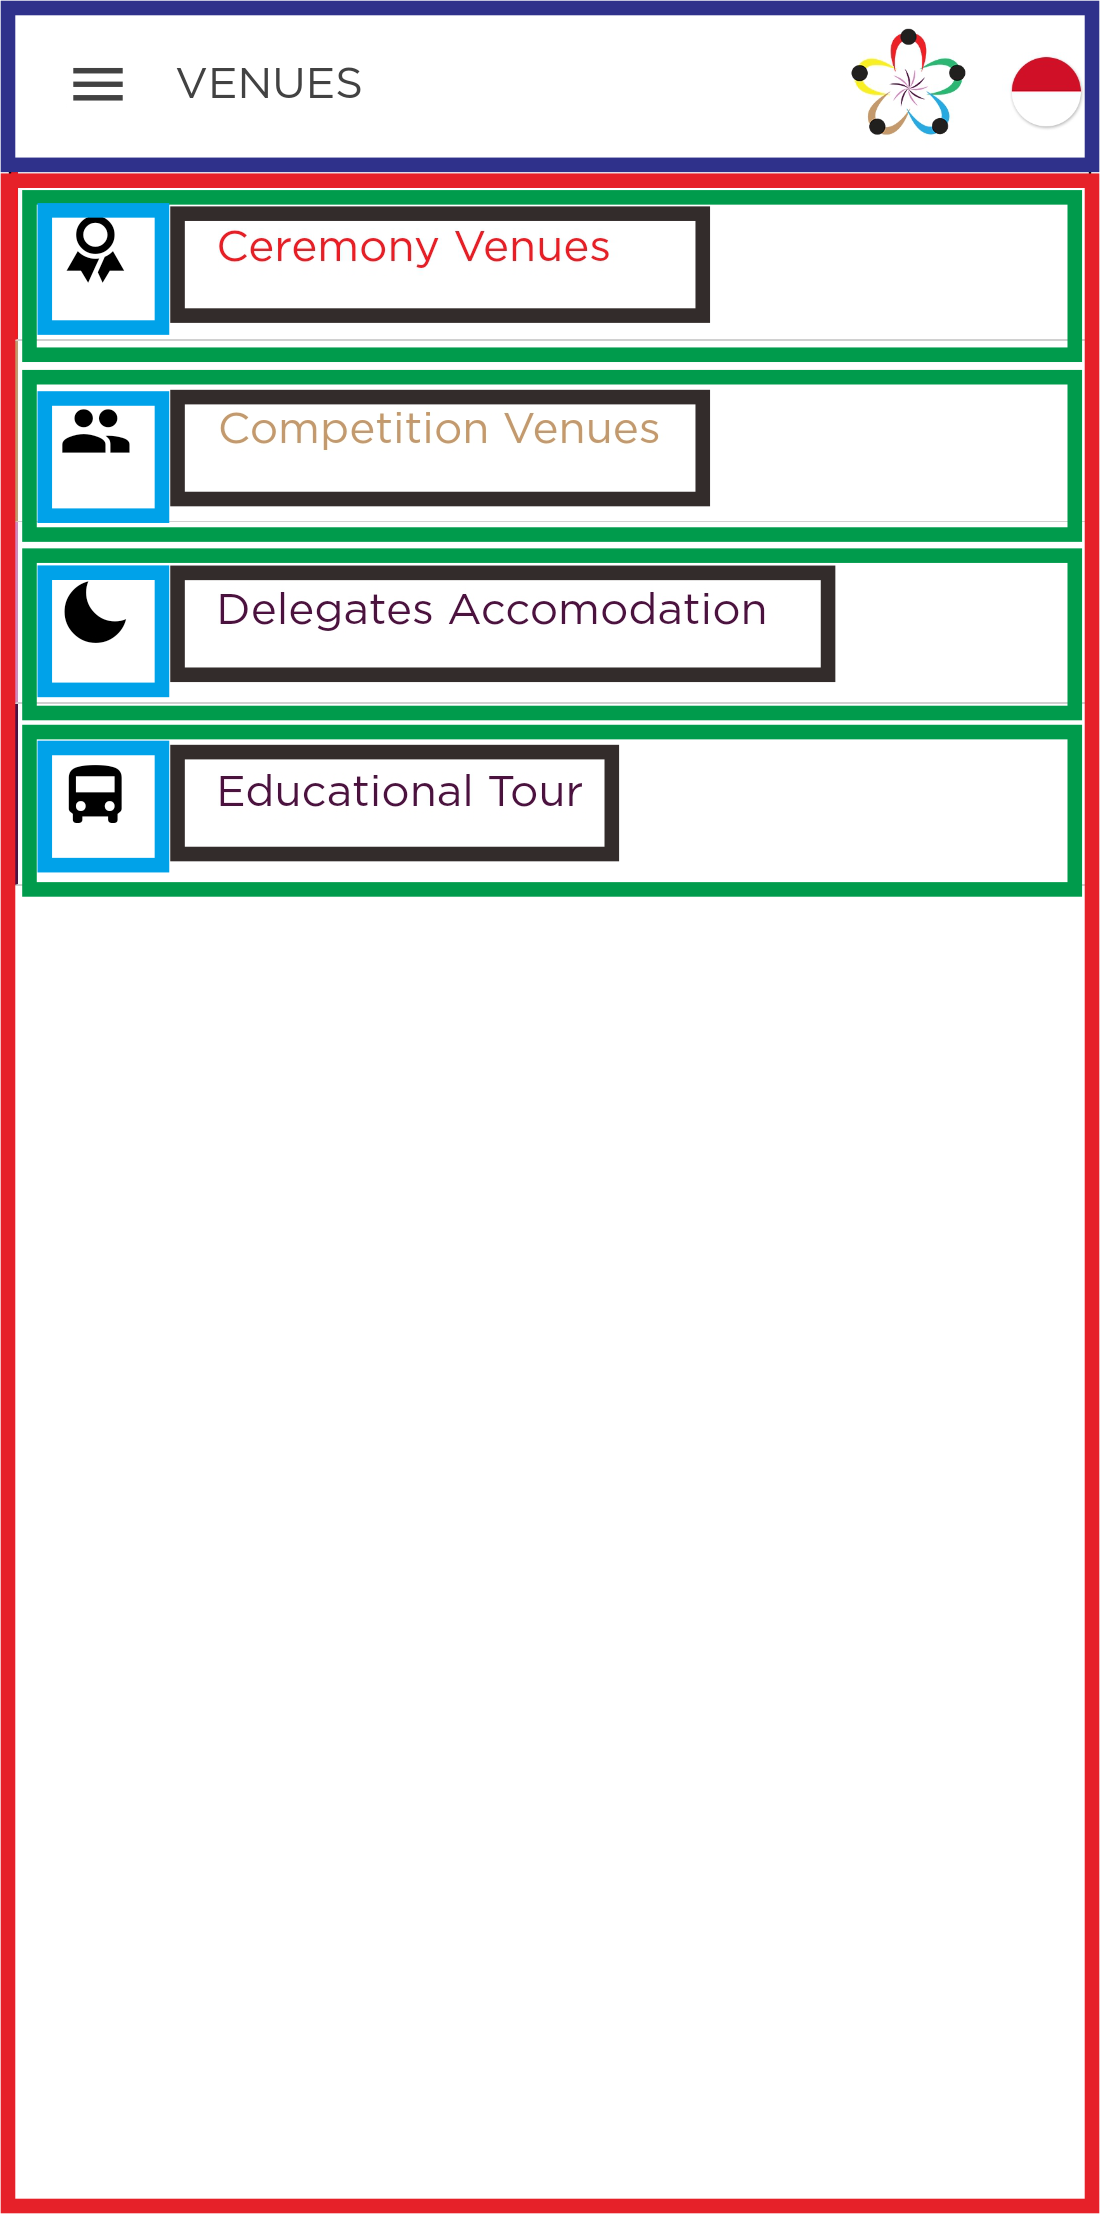
\includegraphics[scale=0.465]{Gambar/VenuePageWireframe.png}
         	\caption{Wireframe Komponen \textit{Venues} Aplikasi WSDC 2017 Bali terdahulu}
         	\label{fig:VenuePageWireframe}
     	\end{subfigure}
     	\hspace*{0.5in}
     	\begin{subfigure}[b]{0.43\textwidth}
         	\centering
         	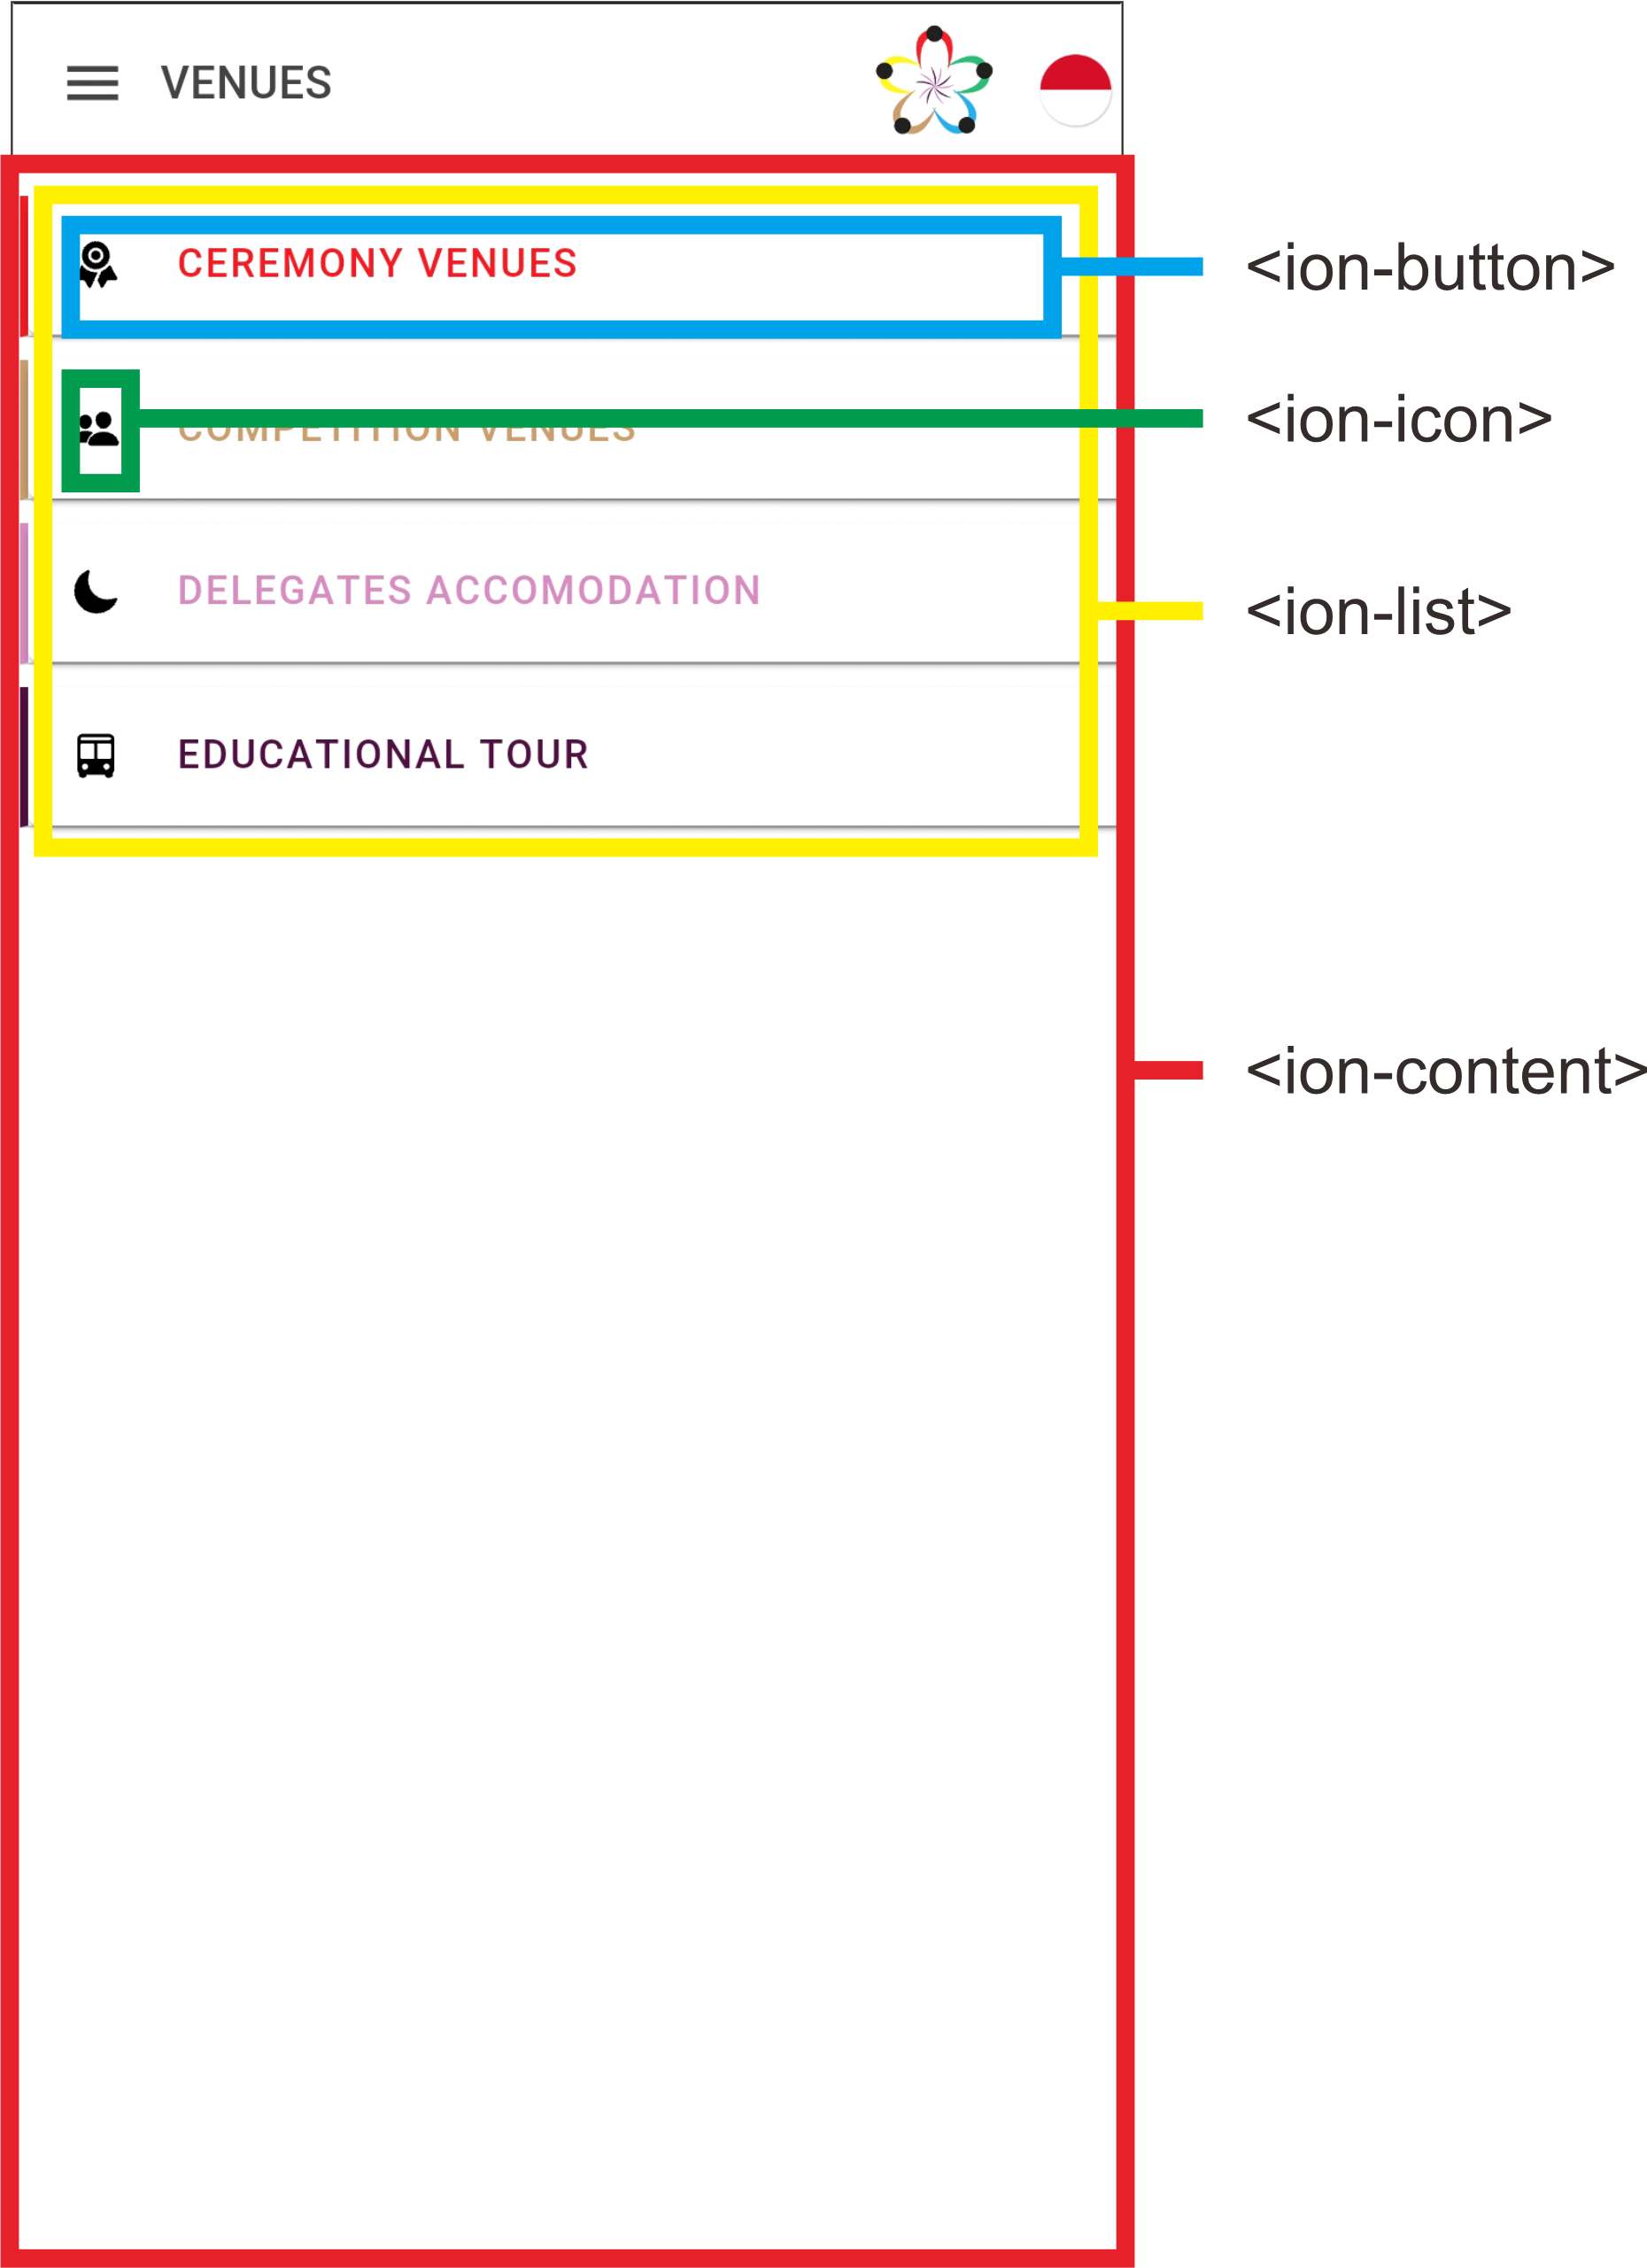
\includegraphics[scale=0.4]{Gambar/VenuePageKini.png}
         	\caption{UI Component Komponen \textit{Venues} Aplikasi WSDC 2017 Bali terbaru}
         	\label{fig:VenuePageKini}
     	\end{subfigure}
        \caption{Komponen \textit{Venues} pada Aplikasi WSDC 2017 Bali}
        \label{fig:UIComponent1}
	\end{figure}
	\begin{enumerate}
		\item Analisis pada Aplikasi WSDC 2017 Bali terdahulu \\
		Komponen ini memiliki sebuah \textit{file} TypeScript untuk mengatur keseluruhan halaman. Di dalam \textit{file} venues.ts terdapat sebuah \textit{decorator} @Component untuk komponen (Kode~\ref{lst:componentVenues}). Di dalam decorator ini terdapat CSS \textit{selector} untuk memilih CSS yang akan digunakan, serta \textbf{templateUrl} untuk mendefinisikan ekxternal HTML \textit{template} yang akan digunakan. \textit{Template} HTML yang digunakan adalah \textit{file} venues.html
	
\begin{lstlisting}[label={lst:componentVenues}, caption=@Component pada venues.ts]
@Component({
  selector: 'page-venues',
  templateUrl: 'venues.html'
})
\end{lstlisting}

	Terdapat kelas VenuesPage yang memiliki satu \textit{constructor}. \textit{Constructor} kelas ini berfungsi untuk mengambil data \textit{venues} yang berada di dalam penyimpanan internal. Data tersebut kemudian disimpan ke dalam variabel lokal valVenues. Terdapat sebuah \textit{method} itemTapped() yang berfungsi untuk berpindah halaman ke halaman venues-map, yang akan menampilkan peta lokasi berlangsungnya acara, sesuai dengan \textit{venues} yang dipilih.

	Terdapat \textit{file} venues.html yang digunakan untuk menampilkan halaman \textit{venues}. Terdapat beberapa komponen yang disediakan oleh Ionic Framework, yang diimplementasikan ke dalam halaman \textit{venues}. Diantaranya adalah sebagai berikut:	
	
	\begin{itemize}
		\item \textit{Header} \\
		Halaman \textit{venues} memiliki \textit{header} dengan \textit{tag} \texttt{<ion-header>} (Kode~\ref{lst:headerVenues}) seperti pada gambar~\ref{fig:VenuePageWireframe}. \textit{Tag} tersebut merupakan komponen \textit{parent} yang menampung komponen navbar yang ditandai dengan kotak berwarna biru. Di dalam navbar tersebut, terdapat sebuah \textit{tag} \texttt{<button>} untuk memunculkan \textit{sidemenu}. Terdapat \textit{tag} \texttt{<ion-title>} sebagai judul dari halaman, yaitu ``Venues''.
		
\begin{lstlisting}[label={lst:headerVenues}, caption=\textit{Header} pada venues.html]
<ion-header>
  <ion-navbar>
    <button ion-button menuToggle>
      <ion-icon name="menu"></ion-icon>
    </button>
    <ion-title>Venues</ion-title>
  </ion-navbar>
</ion-header>
\end{lstlisting}

		\item \textit{Content} \\
		\textit{Content} pada halaman venues memiliki \textit{tag} \texttt{<ion-content>} (Kode~\ref{lst:contentVenues}) yang pada gambar~\ref{fig:VenuePageWireframe} dengan kotak berwarna merah. Di dalam \textit{tag} \texttt{<ion-content>} terdapat sebuah \textit{tag} \texttt{<ion-grid>} dan sebuah \textit{tag} \texttt{<ion-row>}. Di dalam \textit{tag} \texttt{<ion-row>} terdapat sebuah \textit{tag} \texttt{<ion-list>} yang berisi \textit{tag} \texttt{<ion-button>} yang ditandai dengan kotak berwarna hijau pada gambar~\ref{fig:VenuePageWireframe}. Masing-masing \textit{tag} \texttt{<ion-button>} berisi \textit{tag} \texttt{<ion-icon>} yang ditandai dengan kotak berwarna biru muda, dan \textit{tag} \texttt{<span>} berisi nama \textit{venues} yang ditandai dengan kotak berwarna hitam. 
		
\begin{lstlisting}[label={lst:contentVenues}, caption=\textit{Content} pada venues.html]
<ion-content>
  <ion-grid>
    <ion-row>
      <ion-list style="width: 100%;" no-lines>
          <button ion-item  id="{{wsdcVenue.id}}" *ngFor="let wsdcVenue of venuesData" (click)="itemTapped($event, wsdcVenue)">
            <ion-icon ios="ios-{{wsdcVenue.icon}}-outline" md="md-{{wsdcVenue.icon}}" item-start></ion-icon>
            <span>{{wsdcVenue.name}}</span>
          </button>
      </ion-list>
    </ion-row>
  </ion-grid>
</ion-content>
\end{lstlisting}
	\end{itemize}

	Terdapat kelas VenuesPage pada venues.ts. Kelas ini memiliki satu \textit{constructor}. \textit{Constructor} kelas ini berfungsi untuk mengambil data \textit{venues} yang berada di dalam penyimpanan. Data tersebut kemudian disimpan ke dalam variabel lokal venuesData, yang berisi id, \textit{name}, \textit{icon}, geojson, dan colorIdx. 
	Terdapat sebuah \textit{method} yaitu itemTapped(event, wsdcVenue). \textit{Method} ini memiliki dua buah parameter, \textit{event} yang berisi \textit{event} pada \textit{tag button}, dan wsdcVenue yang merupakan data bertipe json yang berisi data lengkap sebuah venue yang ada di penyimpanan sesuai dengan data venue pada \textit{event} di dalam \textit{tag button}. Kemudian, dengan menggunakan NavController milik Ionic Framework, data wsdcVenue dikirimkan ke halaman Venues Map. Setelah itu halaman akan berpindah ke halaman Venues Map.
		\item Perancangan Aplikasi WSDC 2017 Bali terbaru \\
		Pada komponen \textit{venues}, terdapat beberapa UI Component yang akan diimplementasikan seperti pada gambar~\ref{fig:VenuePageKini}, diantaranya adalah sebagai berikut:
		\begin{itemize}
			\item Content \\
		Komponen Content dengan \textit{tag} \texttt{<ion-content>} akan digunakan sebagai penyedia area konten yang digunakan untuk mengontrol area yang dapat digulir dan menampilkan isi konten dari halaman \textit{venues}. UI Component \textit{Content} pada Ionic Framework versi 6 tidak mengalami perubahan~dari~Ionic~Framework~versi~3.
		
			\item \textit{Grid} \\
		Komponen ini akan digunakan untuk membangun tata letak kustom pada halaman info. UI Component \textit{Grid} dengan \textit{tag} \texttt{<ion-grid>} dan {<ion-row>} pada Ionic Framework versi 6 tidak mengalami perubahan dari Ionic Framework versi 3

			\item \textit{List} \\
		\textit{List} dengan \textit{tag} \texttt{<ion-list>}, yang terdiri dari baris yang setiap barisnya berisi kategori \textit{venues} yang disusun menggunakan \textit{button}. UI Component \textit{List} dengan \textit{tag} \texttt{<ion-list>} pada Ionic Framework versi 6 tidak mengalami perubahan dari Ionic Framework versi 3.
		
			\item \textit{Button} \\
		\textit{Button} digunakan untuk berpindah ke halaman \textit{Venues Map} sesuai dengan tombol apa yang dipilih. Pada aplikasi WSDC 2017 Bali saat ini yang menggunakan Ionic 3, komponen ini ditulis menggunakan \textit{tag} \texttt{<button>} (Kode~\ref{lst:buttonVenuesWSDCOld}). Sejak Ionic Framework versi 4, terjadi perubahan dengan mengganti \textit{tag} tersebut menjadi {<ion-button>} pada aplikasi yang akan dibangun yang menggunakan Ionic 6 (Kode~\ref{lst:buttonVenuesWSDCNew}). 
			
		
\begin{lstlisting}[label={lst:buttonVenuesWSDCOld}, caption=\textit{Button} dengan Ionic 3 di Aplikasi WSDC 2017 Bali Saat Ini]
<button ion-item  id="{{wsdcVenue.id}}" *ngFor="let wsdcVenue of venuesData" (click)="itemTapped($event, wsdcVenue)">
	<ion-icon ios="ios-{{wsdcVenue.icon}}-outline" md="md-{{wsdcVenue.icon}}" item-start></ion-icon>
	<span>{{wsdcVenue.name}}</span>
</button>
\end{lstlisting}

\begin{lstlisting}[label={lst:buttonVenuesWSDCNew}, caption=\textit{Button} dengan Ionic 6 di Aplikasi WSDC 2017 Bali yang Akan Dibuat]
<ion-button ion-item  id="{{wsdcVenue.id}}" *ngFor="let wsdcVenue of venuesData" (click)="itemTapped($event, wsdcVenue)">
	<ion-icon ios="ios-{{wsdcVenue.icon}}-outline" md="md-{{wsdcVenue.icon}}" item-start></ion-icon>
	<span>{{wsdcVenue.name}}</span>
</ion-button>
\end{lstlisting}
		
			\item \textit{Icon} \\
		Komponen ini akan digunakan untuk menampilkan ikon pada halaman \textit{venues}. UI Component \textit{Icon} dengan \textit{tag} \texttt{<ion-icon>} pada Ionic Framework versi 6 tidak mengalami perubahan dari Ionic Framework versi 3.
		\end{itemize}	
		
		\item Perancangan Aplikasi WSDC 2017 Bali terbaru \\
		Pada komponen \textit{venues}, terdapat beberapa UI Component yang akan diimplementasikan seperti pada gambar~\ref{fig:VenuePageKini}, diantaranya adalah sebagai berikut:
		\begin{itemize}
			\item Content \\
		Komponen Content dengan \textit{tag} \texttt{<ion-content>} akan digunakan sebagai penyedia area konten yang digunakan untuk mengontrol area yang dapat digulir dan menampilkan isi konten dari halaman \textit{venues}. UI Component \textit{Content} pada Ionic Framework versi 6 tidak mengalami perubahan~dari~Ionic~Framework~versi~3.
		
			\item \textit{Grid} \\
		Komponen ini akan digunakan untuk membangun tata letak kustom pada halaman info. UI Component \textit{Grid} dengan \textit{tag} \texttt{<ion-grid>} dan {<ion-row>} pada Ionic Framework versi 6 tidak mengalami perubahan dari Ionic Framework versi 3

			\item \textit{List} \\
		\textit{List} dengan \textit{tag} \texttt{<ion-list>}, yang terdiri dari baris yang setiap barisnya berisi kategori \textit{venues} yang disusun menggunakan \textit{button}. UI Component \textit{List} dengan \textit{tag} \texttt{<ion-list>} pada Ionic Framework versi 6 tidak mengalami perubahan dari Ionic Framework versi 3.
		
			\item \textit{Button} \\
		\textit{Button} digunakan untuk berpindah ke halaman \textit{Venues Map} sesuai dengan tombol apa yang dipilih. Pada aplikasi WSDC 2017 Bali saat ini yang menggunakan Ionic 3, komponen ini ditulis menggunakan \textit{tag} \texttt{<button>} (Kode~\ref{lst:buttonVenuesWSDCOld}). Sejak Ionic Framework versi 4, terjadi perubahan dengan mengganti \textit{tag} tersebut menjadi {<ion-button>} pada aplikasi yang akan dibangun yang menggunakan Ionic 6 (Kode~\ref{lst:buttonVenuesWSDCNew}). 
			
		
\begin{lstlisting}[label={lst:buttonVenuesWSDCOld}, caption=\textit{Button} dengan Ionic 3 di Aplikasi WSDC 2017 Bali Saat Ini]
<button ion-item  id="{{wsdcVenue.id}}" *ngFor="let wsdcVenue of venuesData" (click)="itemTapped($event, wsdcVenue)">
	<ion-icon ios="ios-{{wsdcVenue.icon}}-outline" md="md-{{wsdcVenue.icon}}" item-start></ion-icon>
	<span>{{wsdcVenue.name}}</span>
</button>
\end{lstlisting}

\begin{lstlisting}[label={lst:buttonVenuesWSDCNew}, caption=\textit{Button} dengan Ionic 6 di Aplikasi WSDC 2017 Bali yang Akan Dibuat]
<ion-button ion-item  id="{{wsdcVenue.id}}" *ngFor="let wsdcVenue of venuesData" (click)="itemTapped($event, wsdcVenue)">
	<ion-icon ios="ios-{{wsdcVenue.icon}}-outline" md="md-{{wsdcVenue.icon}}" item-start></ion-icon>
	<span>{{wsdcVenue.name}}</span>
</ion-button>
\end{lstlisting}
		
			\item \textit{Icon} \\
		Komponen ini akan digunakan untuk menampilkan ikon pada halaman \textit{venues}. UI Component \textit{Icon} dengan \textit{tag} \texttt{<ion-icon>} pada Ionic Framework versi 6 tidak mengalami perubahan dari Ionic Framework versi 3.
		\end{itemize}	
	\end{enumerate}
	\newpage
	\item Komponen \textit{Venues Map} \\
	Komponen \textit{Venues Map} digunakan untuk menampilkan halaman \textit{Venues Map} yang berisi peta untuk masing-masing lokasi \textit{venue}, serta jarak dari posisi pengguna ke tiap-tiap lokasi \textit{venue}. 
	\begin{figure}[H]
    	\centering
     	\begin{subfigure}[b]{0.43\textwidth}
        	\centering
         	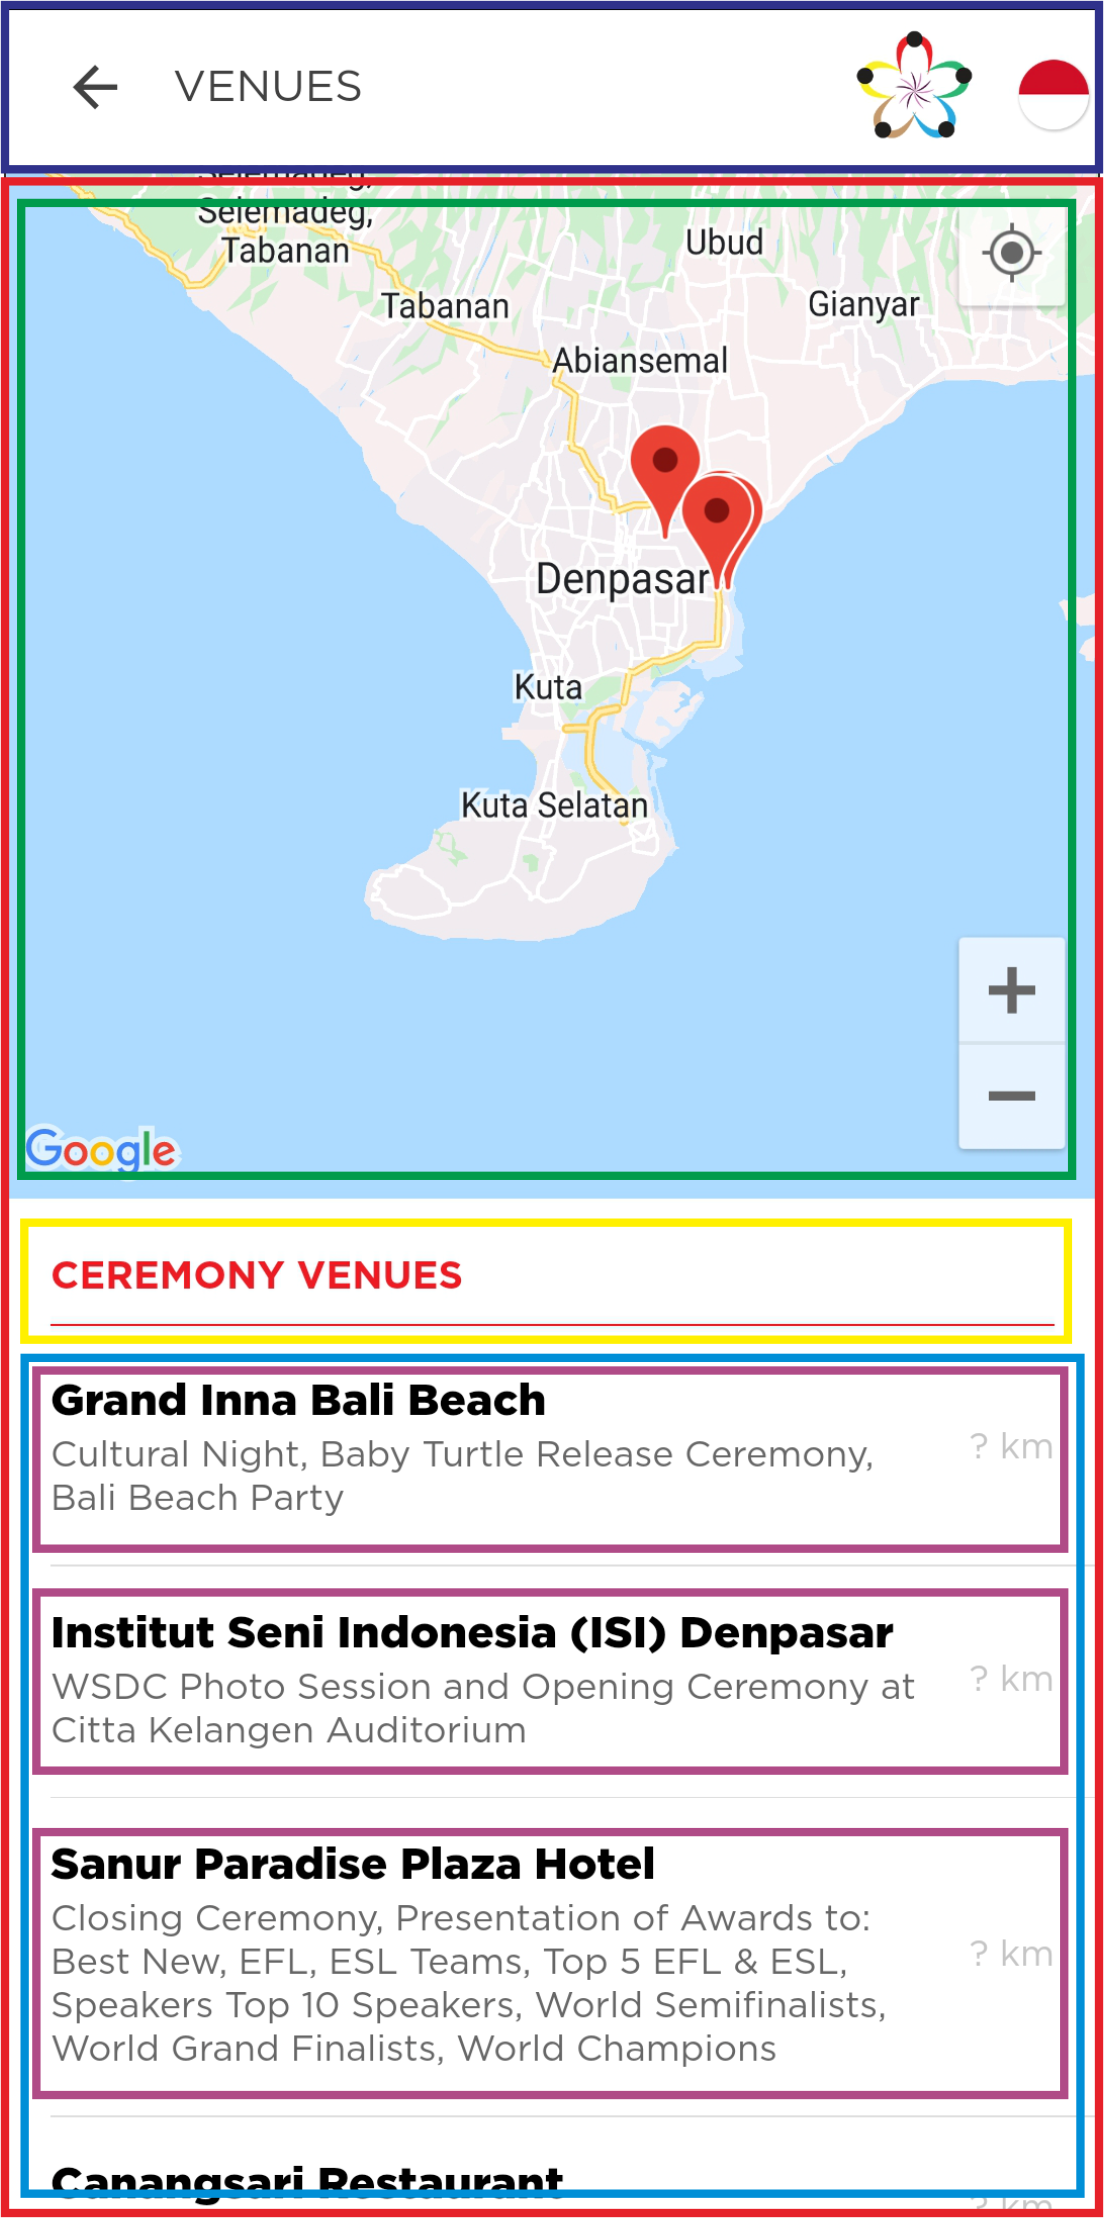
\includegraphics[scale=0.465]{Gambar/VenueMapPageWireframe.png}
         	\caption{Wireframe Komponen \textit{Venues Map} Aplikasi WSDC 2017 Bali terdahulu}
         	\label{fig:VenueMapPageWireframe}
     	\end{subfigure}
     	\hspace*{0.5in}
     	\begin{subfigure}[b]{0.43\textwidth}
         	\centering
         	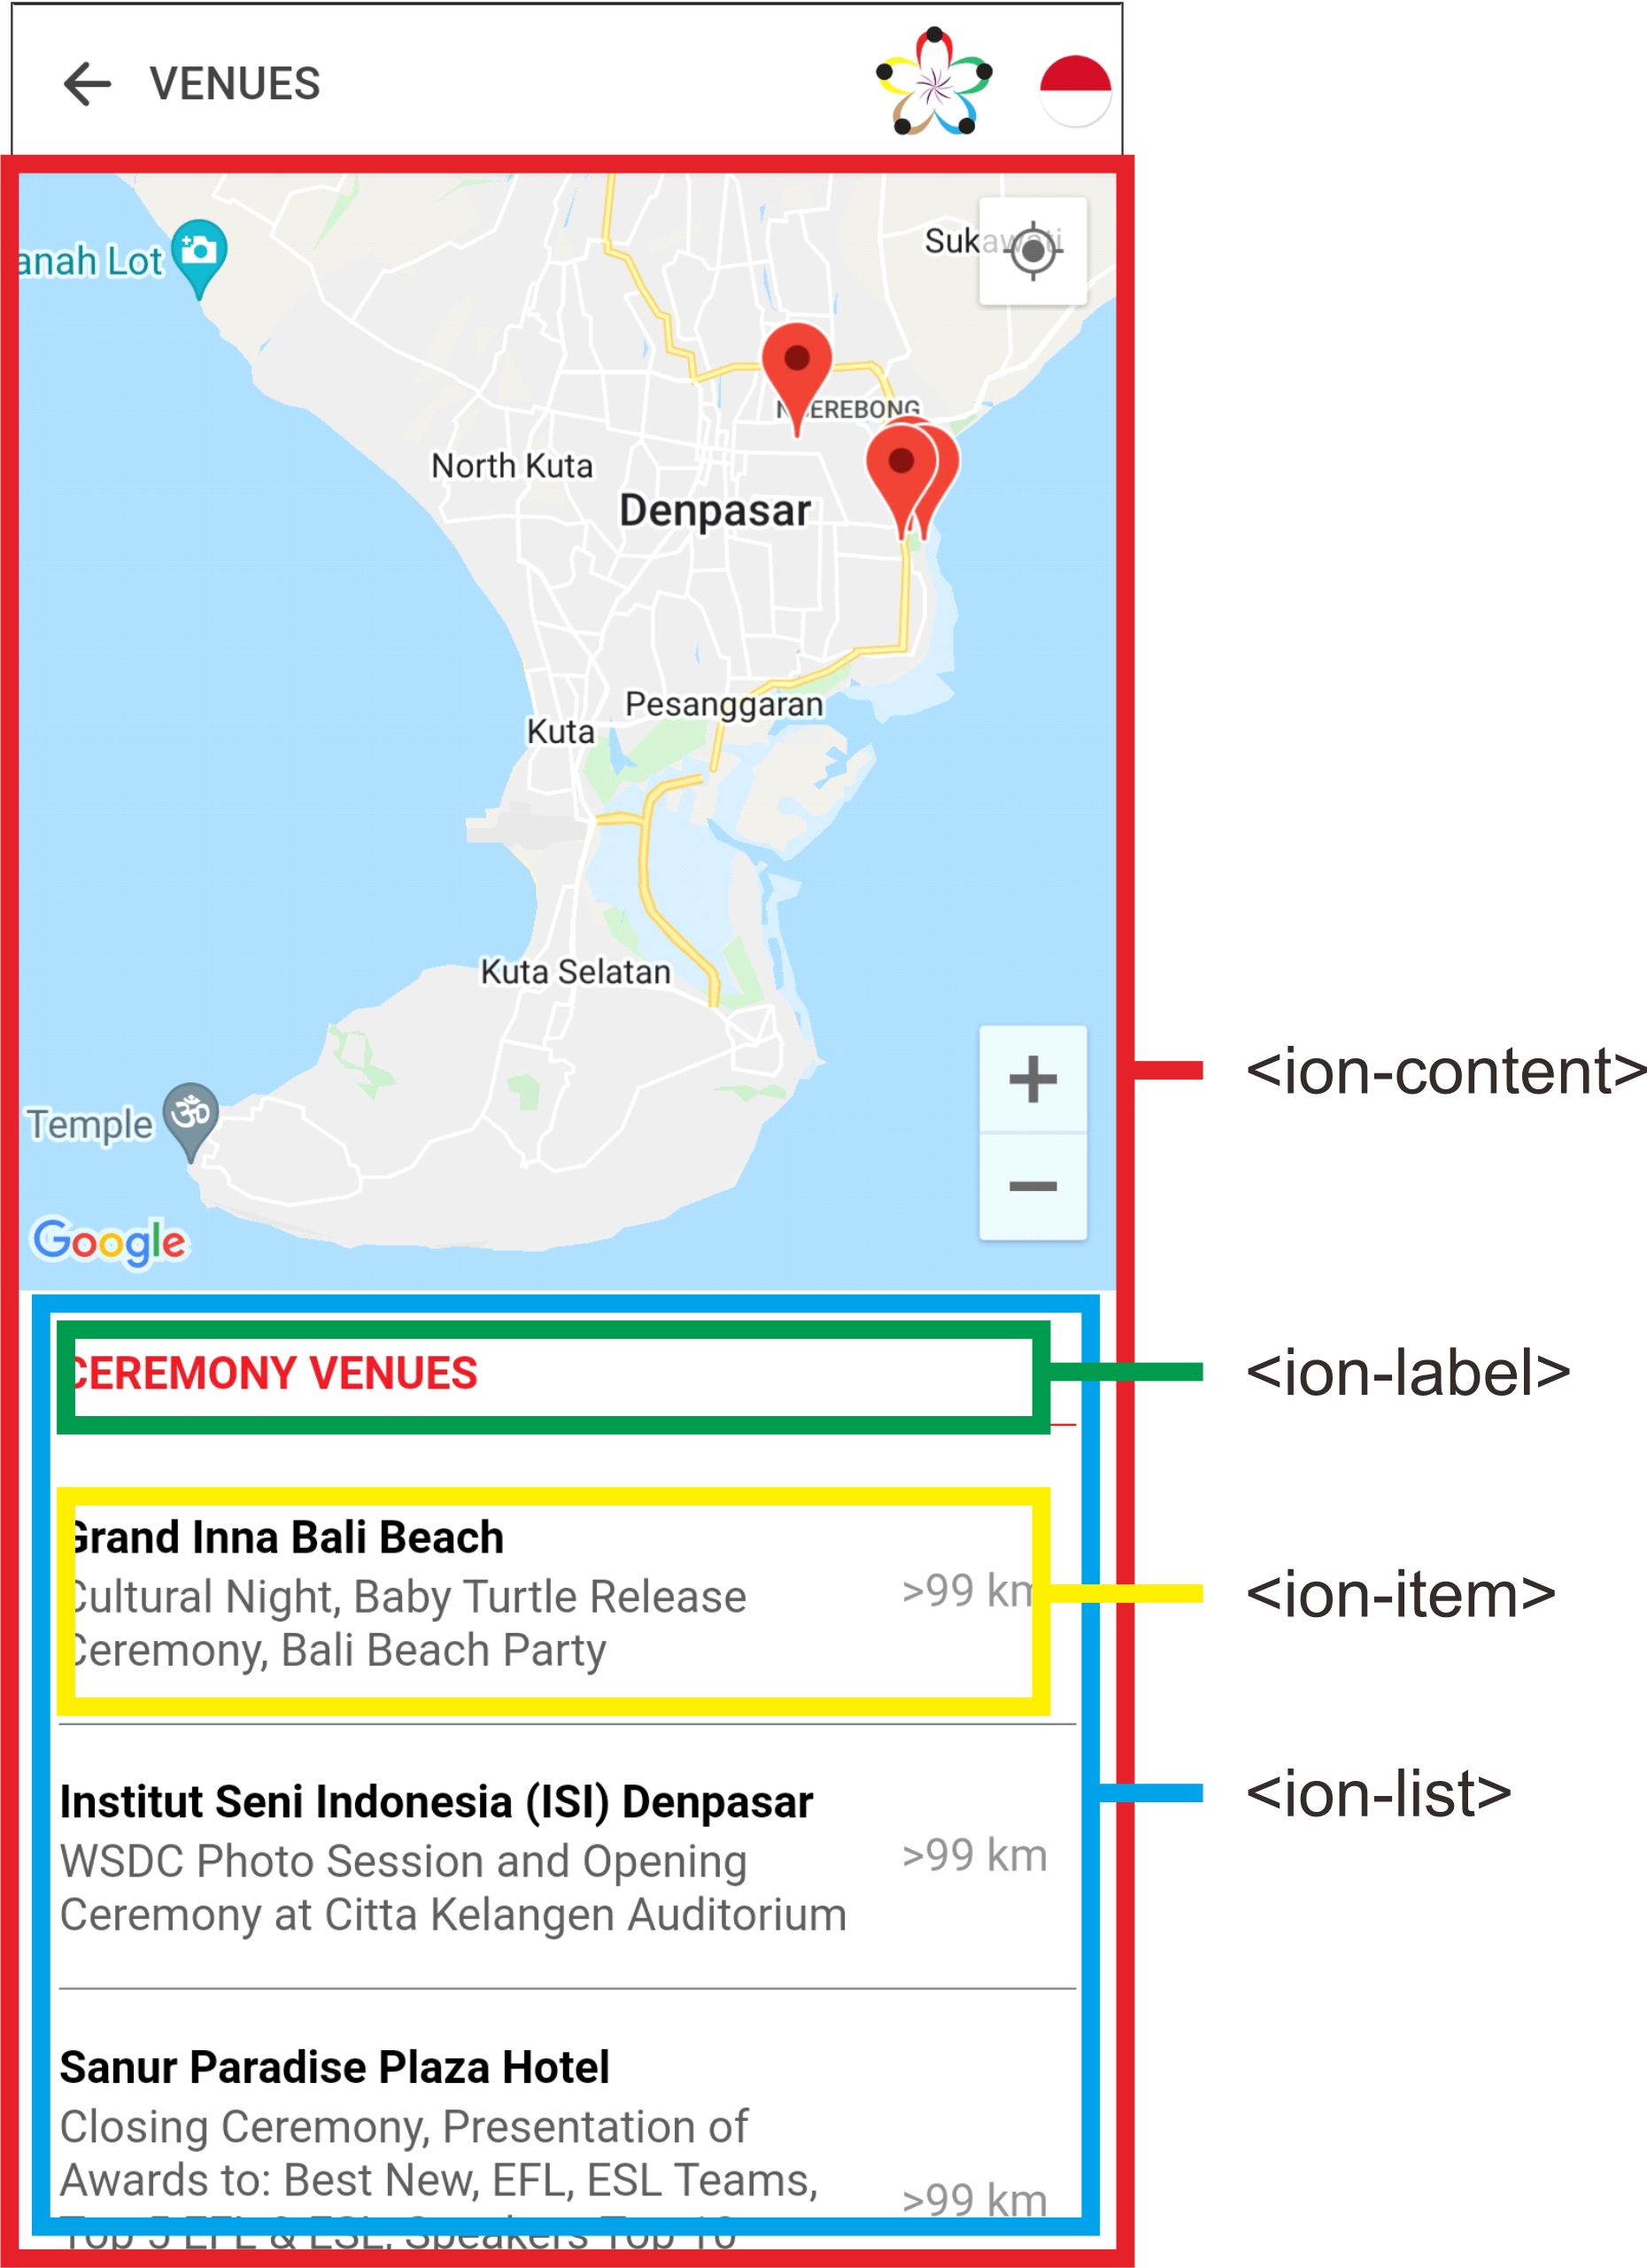
\includegraphics[scale=0.4]{Gambar/VenueMapKini.png}
         	\caption{UI Component Komponen \textit{Venues Map} Aplikasi WSDC 2017 Bali terbaru}
         	\label{fig:VenueMapKini}
     	\end{subfigure}
        \caption{Komponen \textit{Venues Map} pada Aplikasi WSDC 2017 Bali}
        \label{fig:UIComponent1}
	\end{figure}
	\begin{enumerate}
		\item Analisis pada Aplikasi WSDC 2017 Bali terdahulu \\
		Komponen \textit{Venues Map} menampilkan sebuah peta yang berisi lokasi dari acara WSDC 2017 Bali. Komponen ini memiliki sebuah \textit{file} TypeScript untuk mengatur keseluruhan halaman. Di dalam \textit{file} venues\textunderscore map.ts terdapat sebuah \textit{decorator} @Component untuk komponen (Kode~\ref{lst:componentVenuesMap}). Di dalam decorator ini terdapat CSS \textit{selector} untuk memilih CSS yang akan digunakan, serta \textbf{templateUrl} untuk mendefinisikan ekxternal HTML \textit{template} yang akan digunakan. \textit{Template} HTML yang digunakan adalah \textit{file} venues\textunderscore map.html
	
\begin{lstlisting}[label={lst:componentVenuesMap}, caption=@Component pada venues\textunderscore map.ts]
@Component({
  selector: 'page-venuesmap',
  templateUrl: 'venues_map.html',
})
\end{lstlisting}	

	Terdapat kelas VenuesMapPage di dalam app.module.ts. Kelas ini memiliki sebuah \textit{constructor}. \textit{Constructor} kelas ini berfungsi untuk mengambil data \textit{venues} yang berada di dalam penyimpanan internal, kemudian disimpan ke dalam variabel lokal venuesData. Di dalam \textit{constructor} mengambil data yang dikirimkan oleh halaman Venues. Data tersebut kemudian dimasukkan ke dalam variabel lokal bernama items. 	
	\newpage
	Pada komponen ini, terdapat sebuah \textit{plugin} Google Maps, yang digunakan untuk menampilkan peta yang berisi lokasi dari kegiatan WSDC 2017 Bali. \textit{Plugin} yang digunakan adalah \textit{plugin} Google Maps yang disediakan oleh Cordova. \textit{Plugin} tersebut diinisialisasikan di dalam \textit{constructor}. Terdapat juga sebuah \textit{plugin} Geolocation, yang berfungsi untuk menerima masukan posisi dari lokasi pengguna yang berisi \textit{latitude} dan \textit{longitude}, yang kemudian keseluruhan lokasi tersebut pada \textit{constructor} akan dihitung jaraknya dari lokasi pengguna saat ini. 
	
	Terdapat beberapa \textit{method} yang digunakan, diantaranya yaitu:
	
	\begin{itemize}
		\item ngAfterViewInit()\\
		\textit{Method} ini dipanggil hanya sekali ketika Angular menyelesaikan inisialisasi tampilan komponen. \textit{Method} ini digunakan untuk menambahkan atribut ke dalam judul dari halaman, yaitu menambahkan warna pada teks judul.
	
		\item loadMap() \\
		\textit{Method} ini dipanggil di dalam \textit{constructor}, dan berfungsi untuk menampilkan peta dengan bantuan \textit{plugin} Google Maps. Pada \textit{method} ini, peta pertama kali akan dibuat dengan pengaturan kamera yang mengarah ke lokasi latitude dan longitude dari kota Kuta, Bali. 	
		\textit{Plugin} Google Maps sendiri akan memanfaatkan fitur-fifur \textit{native} dari suatu perangkat. Fitur-fitur tersebut adalah untuk melakukan \textit{gesture} seperti \textit{scroll}, \textit{tilt}, \textit{rotate}, dan \textit{zoom}. Terdapat fitur untuk menagkses kontrol pada Google Maps, seperti mengakses kompas, tombol lokasi pengguna saat ini, dan melihat peta di dalam ruangan. Saat Google Maps sudah tersedia untuk digunakan, \textit{method} ini akan memanggil \textit{method} loadMarkers() untuk membuat penanda pada peta.	
		\item loadMarkers() \\
		\textit{Method} ini dipanggil oleh \textit{method} loadMap(). \textit{Method} ini digunakan untuk menampilkan \textit{marker} dari setiap lokasi acara WSDC 2017 Bali yang sudah tersimpan di dalam variabel items. Google Maps menggunakan lokasi latitude dan longitude dari suatu lokasi yang berada di variabel items untuk membuat \textit{marker}.  
		\item featTapped(event, index) \\
		\textit{Method} ini merupakan sebuah \textit{template statement} dipanggil oleh \textit{event} di dalam \textit{tag} \texttt{<ion-item>} pada venues\textunderscore map.html yaitu \textit{event} (click). Saat pengguna melakukan klik di dalam \textit{tag} \texttt{<ion-item>}, maka peta akan melakukan \textit{zoom} sesuai dengan lokasi yang ada pada \textit{tag} \texttt{<ion-item>}.
		\item computeDistance(p1, p2)\\
		\textit{Method} ini digunakan untuk menghitung jarak antara pengguna ke lokasi \textit{venues}. \textit{Method} ini memanfaatkan fitur dari \textit{plugin} Google Maps, yaitu computeDistanceBetween dengan parameter lokasi \textit{venues} dan lokasi perangkat pengguna yang didapatkan dari paramter \textit{method} ini.
	\end{itemize}
	
	Terdapat \textit{file} venues\textunderscore map.html yang digunakan untuk menampilkan halaman \textit{venues map}. Terdapat beberapa komponen yang disediakan oleh Ionic Framework, yang diimplementasikan ke dalam halaman. Diantaranya adalah sebagai berikut:
\newpage
	\begin{itemize}
		\item \textit{Header} \\
		 Halaman \textit{venues} memiliki \textit{header} dengan \textit{tag} \texttt{<ion-header>} (Kode~\ref{lst:headerVenuesMap}) seperti pada gambar~\ref{fig:VenueMapPageWireframe}. \textit{Tag} tersebut merupakan komponen \textit{parent} yang menampung komponen navbar seperti yang ditandai dengan kotak berwarna biru. Di dalam navbar, terdapat sebuah \textit{tag} \texttt{<button>} untuk memunculkan \textit{sidemenu} dan \texttt{<ion-icon>} untuk menampilkan icon. Terdapat \textit{tag} \texttt{<ion-title>}~sebagai~judul~dari~halaman,~yaitu~``Venues''.
		
\begin{lstlisting}[label={lst:headerVenuesMap}, caption=\textit{Header} pada venues\textunderscore map.html]
<ion-header>
  <ion-navbar>
    <button ion-button menuToggle>
      <ion-icon name="menu"></ion-icon>
    </button>
    <ion-title>Venues</ion-title>
  </ion-navbar>
</ion-header>
\end{lstlisting}

		\item \textit{Content} \\
		\textit{Content} pada halaman venues dibungkus oleh \textit{tag} <ion-content> (Kode~\ref{lst:contentVenuesMap}) yang pada gambar~\ref{fig:VenuePageWireframe} dengan kotak berwarna merah. Di dalam \textit{tag} \texttt{<ion-content>} terdapat sebuah \textit{tag} \texttt{<div>} dengan id bernilai map, untuk menampilkan peta lokasi dari \textit{venues} seperti yang ditandai dengan kotak berwarna hijau pada gambar~\ref{fig:VenueMapPageWireframe}. Untuk judul dari \textit{venues} ditandai dengan kotak berwarna kuning dengan menggunakan \textit{tag} \texttt{<h3>}. Terdapat sebuah \textit{tag} \texttt{<ion-scroll>} seperti yang ditandai dengan kotak berwarna biru muda, berfungsi untuk menampilkan sebuah konten yang dapat digulir. Di dalam \textit{tag} \texttt{<ion-scroll>} terdapat sebuah \textit{tag} \texttt{<ion-list>} dan \texttt{<ion-item>} seperti yang ditandai dengan kotak berwarna ungu, berisi nama, deskripsi, serta jarak pengguna ke tempat \textit{venues} berada. \textit{Tag} \texttt{<ion-item>} akan melakukan perulangan dengan menggunakan \texttt{*ngFor} yang tersedia pada Angular untuk menampilkan daftar \textit{venues}.
		
\begin{lstlisting}[label={lst:contentVenuesMap}, caption=\textit{Content} pada venues\textunderscore map.html]
<ion-content>
  <div #map id="map"></div>
  <h3 #pagetitle>
    {{selectedItem.name}}
  </h3>
  <ion-scroll scrollY="true">
    <ion-list>
      <ion-item text-wrap *ngFor="let feature of items; let i=index" (click)="featTapped($event, i)">
        <h2>{{feature.name}}</h2>
        <p>{{feature.description}}</p>
        <ion-note item-end>
          {{feature.distance}}
        </ion-note>
      </ion-item>
    </ion-list>
  </ion-scroll>
</ion-content>
\end{lstlisting}

	\end{itemize}
		\item Perancangan Aplikasi WSDC 2017 Bali terbaru \\
		Pada komponen \textit{venues map}, terdapat beberapa UI Component yang akan diimplementasikan seperti pada gambar~\ref{fig:VenueMapKini}, diantaranya adalah sebagai berikut:
	\begin{itemize}
			\item Content \\
		Komponen ini akan digunakan sebagai penyedia area konten yang digunakan untuk mengontrol area yang dapat digulir dan menampilkan isi konten dari halaman \textit{venues\textunderscore map}. UI Component \textit{Content} dengan \textit{tag} \texttt{<ion-content>} pada Ionic Framework versi 6 tidak mengalami perubahan dari Ionic Framework versi 3.

			\item \textit{Scroll} \\
			\textit{Tag} \texttt{<ion-scroll>} telah dihapus sejak Ionic Framework versi 4, dan digantikan penggunaannya dengan hanya cukup menggunakan \textit{tag} \texttt{<ion-content>} sejak Ionic Framework versi 4.
		
			\item \textit{List} \\
		\textit{List} dengan \textit{tag} \texttt{<ion-list>}, yang terdiri dari baris yang setiap barisnya berisi nama dan lokasi \textit{venues} yang disusun menggunkan \texttt{<ion-item>}. UI Component \textit{List} dengan \textit{tag} \texttt{<ion-list>} dan \texttt{<ion-item>} pada Ionic Framework versi 6 tidak mengalami perubahan dari Ionic Framework versi 3.
		\end{itemize}
	\end{enumerate}
	
\end{enumerate}
Sebagai penyedia \textit{interface} untuk mengakses SDK \textit{native} dan API \textit{native} pada perangkat, pada skripsi ini akan menggunakan Capacitor dibandingkan dengan Cordova. Capacitor mengelola \textit{plugin} dengan cara yang berbeda dibandingkan dengan Cordova, yaitu dengan cara membangun semua \textit{plugin} sebagai sebuah \textit{libraries} di Android, dan diinstal menggunakan \textit{management tool} adnroid, yaitu Gradle. Capacitor didukung langsung oleh Ionic, dengan pengembangan yang lebih baru dibandingkan Cordova dapat lebih mendukung untuk \textit{Web Apps} modern untuk membuka fungsionalitas~\textit{native}~dari~platform~melalui~API.

Dengan digunakannya Capacitor, maka akan digunakan Capacitor \textit{plugin} diantaranya yaitu:

\begin{itemize}
	\item Capacitor Browser API \\	
	\textit{Plugin} ini berfungsi untuk menjalankan kemampuan \textit{in-app browser} pada aplikasi WSDC 2017 Bali, yaitu untuk membuka berita terkait acara WSDC 2017 Bali. Untuk membuka \textit{in-app browser}, digunakan \textit{method} open() dengan properi url sebagai url yang dituju, seperti pada kode~\ref{lst:methodOpenBrowserAPI}.
	
\begin{lstlisting}[label={lst:methodOpenBrowserAPI}, caption=\textit{Method} open() Pada Browser API]
launch(newsUrl: string) {
	Browser.open({ url: newsUrl });
}
\end{lstlisting}
	
	\item Capacitor Community Google Maps \\
	\textit{Plugin} ini berfungsi untuk menampilkan peta Google Maps secara \textit{native} pada perangkat pengguna. Peta tersebut berisi lokasi dari seluruh acara WSDC 2017 Bali dilaksanakan yang ditandai dengan \textit{marker}, dan juga menampilkan posisi dari perangkat pengguna. Seperti yang sudah dijelaskan pada sub bab~\ref{subsec:capacitor}, Capacitor Community Google Maps membutuhkan sebuah kontainer pada HTML untuk ditempati. Contoh kontainer tersebut seperti pada gambar~\ref{fig:VenuesMapPageKontainer} yang ditandai dengan kotak berwarna merah. Kode HTML untuk kontainer seperti pada kode~\ref{lst:htmlkontainergooglemap} dibuat dengan ukuran lebar sesuai dengan layar ponsel pengguna, dan tinggi sebesar 400px. Kemudian mengisi \textit{option} boundingRect pada \textit{method} createMap() seperti pada kode~\ref{lst:createMapGoogleMaps} dengan nilai yang diambil dari kontainer pada HTML yang sudah dibuat sebelumnya. Dengan begitu, Google Maps sudah memiliki tempat di dalam kontainer pada HTML. Peta Google Maps menampilkan lokasi awal Kuta, Bali dengan memasukan \textit{latitude} dan \textit{longitude} dari Kuta, Bali ke dalam \textit{option} cameraPosition properti target. Selain properti target, digunakan juga properti zoom yang digunakan untuk seberapa besar peta ditampilkan. Semakin besar nilai zoom, maka peta ditampilkan semakin dekat, begitu pula sebaliknya.
	
\begin{lstlisting}[label={lst:htmlkontainergooglemap}, caption=Kontainer pada HTML untuk Peta Capacitor CommunityGoogle Maps]
<div id="container">
  <div id="mapContainer"></div>
</div>
\end{lstlisting}

\begin{lstlisting}[label={lst:createMapGoogleMaps}, caption=\textit{Method} createMap() Pada Capacitor Community Google Maps]
const result = await CapacitorGoogleMaps.createMap({
	boundingRect: {
		width: Math.round(boundingRect.width),
        height: Math.round(boundingRect.height),
        x: Math.round(boundingRect.x),
        y: Math.round(boundingRect.y),
    },
    cameraPosition: {
        target: {
        	latitude: -8.722396,
            longitude: 115.17671,
        },
        zoom: 11,
    },
    preferences: {
        controls: {
    	    isCompassButtonEnabled: true,
            isMyLocationButtonEnabled: true,
            isZoomButtonsEnabled: true,
        },
        appearance: {
            isMyLocationDotShown: true,
        },
    },
});
\end{lstlisting}

\begin{figure}[H]
     \centering
     \begin{subfigure}[b]{0.3\textwidth}
         \centering
         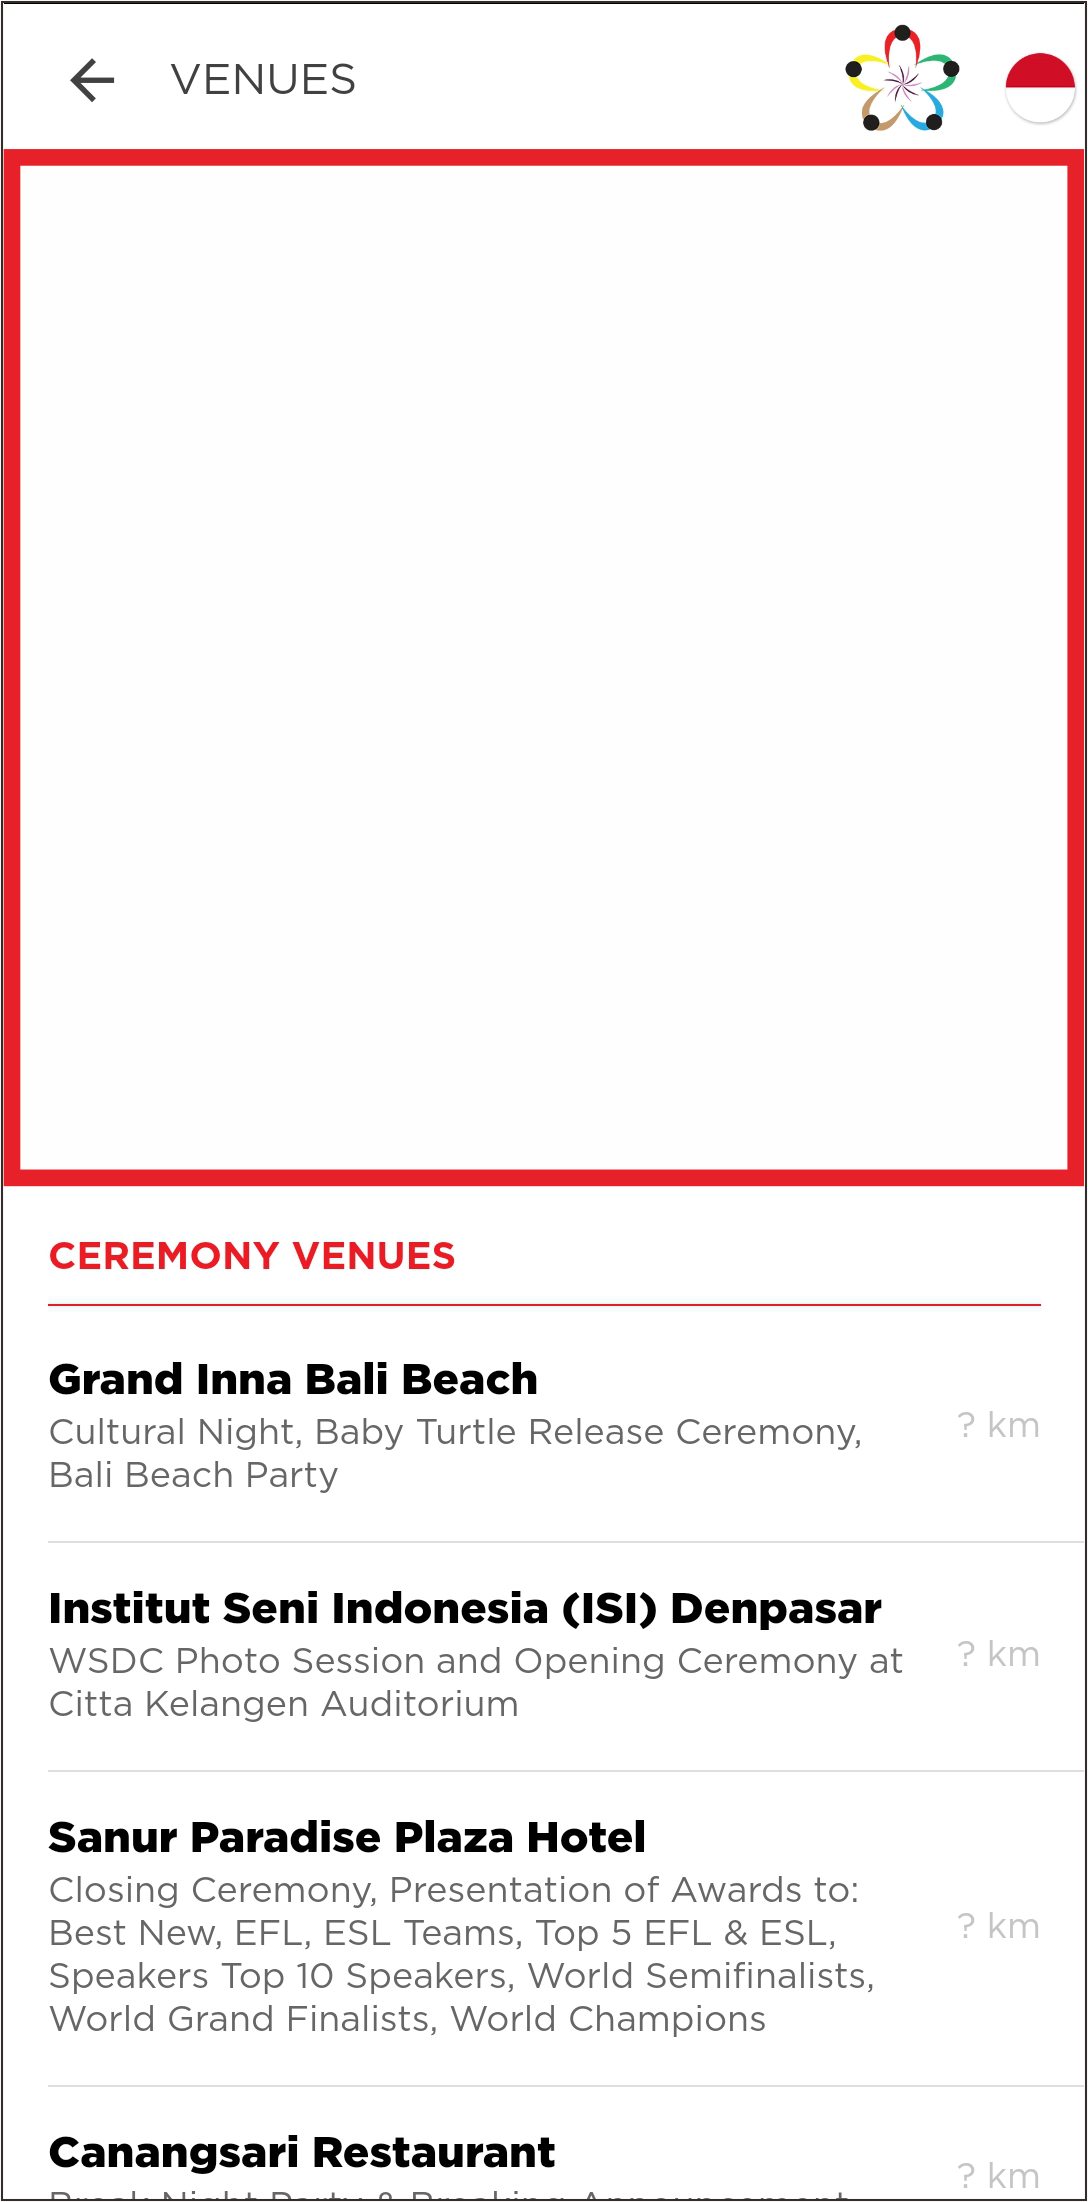
\includegraphics[width=\textwidth]{Gambar/VenuesMapPageKontainer.png}
         \caption{Kontainer untuk Google Maps}
         \label{fig:VenuesMapPageKontainer}
     \end{subfigure}
     \hspace*{0.5in}
     \begin{subfigure}[b]{0.3\textwidth}
         \centering
         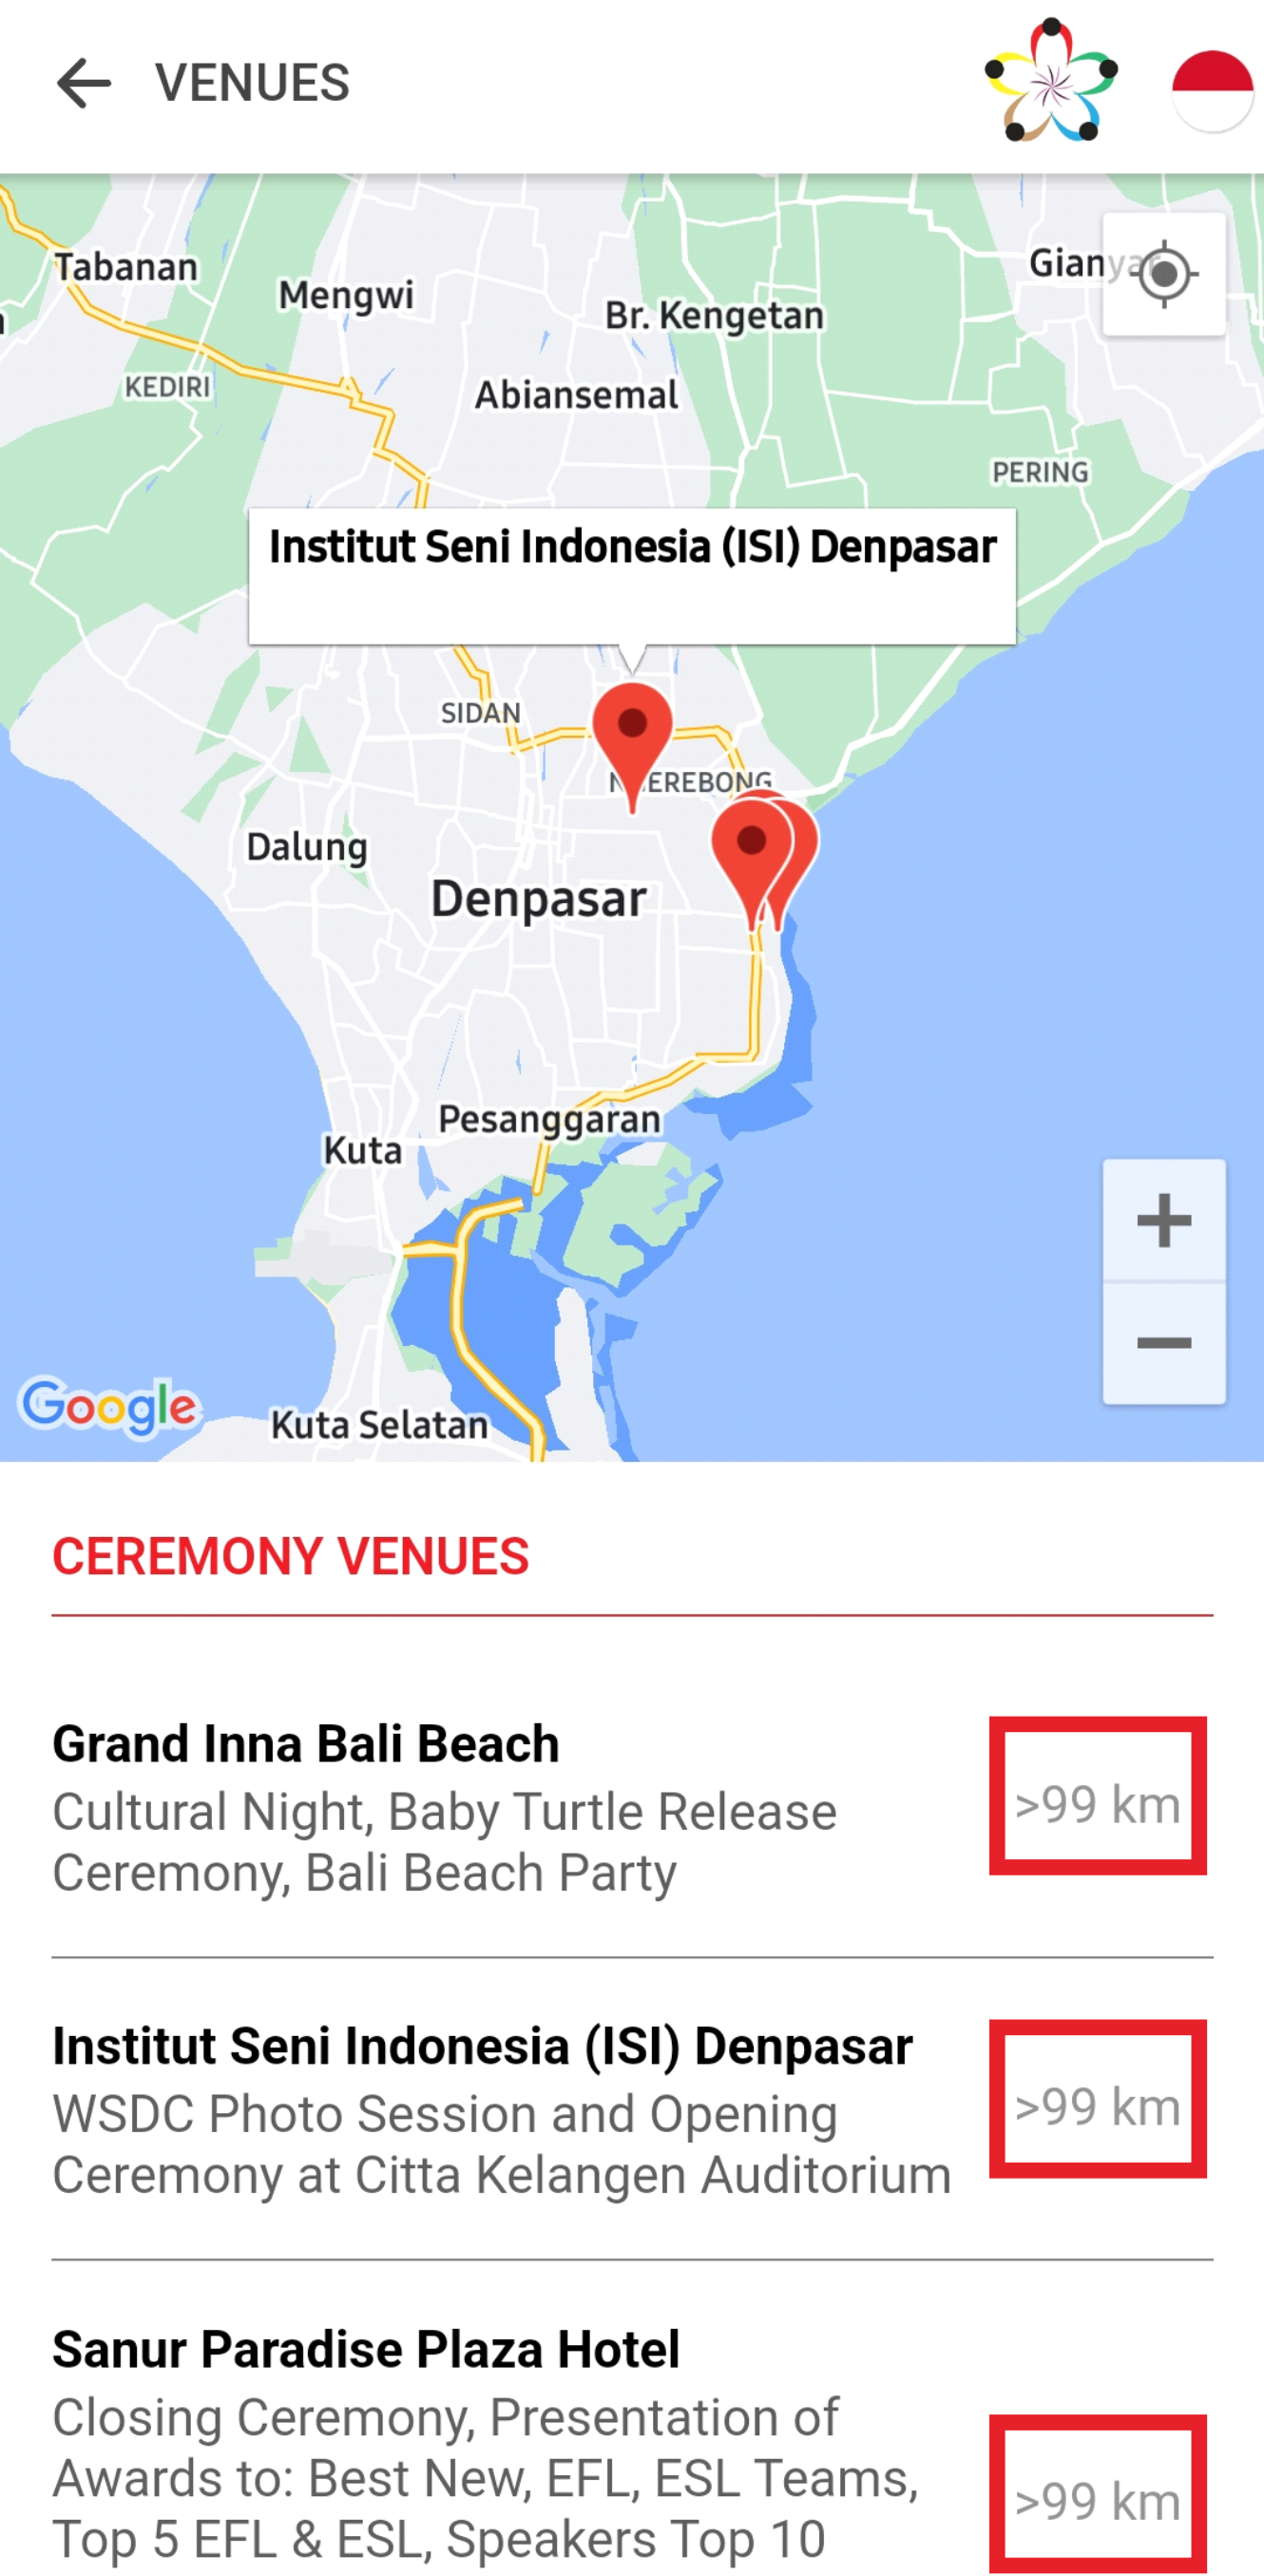
\includegraphics[width=\textwidth]{Gambar/jarakVenuesMap.png}
         \caption{Penggunaan Geolocation}
         \label{fig:jarakVenuesMap}
     \end{subfigure}
        \caption{Penggunaan Community Google Maps dan Geolocation pada Aplikasi WSDC 2017 Bali}
        \label{fig:VenuesMapPenggunaan}
\end{figure}
	
	Pada Capacitor Community Google Maps terdapat \textit{option} preferences seperti pada kode~\ref{lst:createMapGoogleMaps} yang digunakan untuk menambah fungsi pada Google Maps, diantaranya yaitu:
	
	\begin{enumerate}
		\item isCompassButtonEnabled: Digunakan untuk menampilkan tombol kompas sebagai petunjuk arah mata angin.
		\item isMyLocationButtonEnabled: Digunakan untuk menampilkan tombol gps. Ketika tombol tersebut ditekan, posisi peta mengarah pada posisi ponsel pengguna. Penggunaan isMyLocationButtonEnabled adalah pada gambar~\ref{fig:VenueMapPageOption1} yang ditunjukan dengan kotak berwarna hijau.
		\item isZoomButtonsEnabled: Digunakan untuk menampilkan tombol \textit{zoom in} dan \textit{zoom out}. Ketika tombol tersebut ditekan, maka peta akan melakukan \textit{zoom in} dan \textit{zoom out} sesuai dengan tombol yang ditekan. Penggunaan isMyLocationButtonEnabled adalah pada gambar~\ref{fig:VenueMapPageOption1} yang ditunjukan dengan kotak berwarna kuning.
		\item isMyLocationDotShown: Digunakan untuk menampilkan titik biru sebagai tanda lokasi pengguna saat ini. Titik ini akan muncul ketika peta mengarah pada posisi ponsel pengguna. Penggunaan isMyLocationButtonEnabled adalah pada gambar~\ref{fig:VenueMapPageOption2} yang ditunjukan dengan kotak berwarna biru.
	\end{enumerate}
	
	Di dalam peta Google Maps menampilkan \textit{marker} untuk setiap lokasi \textit{venue} seperti pada gambar~\ref{fig:VenueMapPageOption1} yand ditandai dengan kotak warna hitam. Untuk menampilkan \textit{marker} digunakan \textit{method} addMarker() seperti pada kode~\ref{lst:markergooglemap}. \textit{Marker} ditempatkan pada lokasi \textit{venue} sesuai dengan koordinat \textit{latitude} dan \textit{longitude} masing-masing \textit{venue}. Lokasi tersebut ditambahkan pada \textit{option} position. Terdapat juga \textit{option} preferences yang memiliki properti \textit{title}, digunakan untuk menampilkan nama \textit{venue} diatas \textit{marker} ketika \textit{marker} ditekan seperti pada gambar~\ref{fig:VenueMapPageOption1} yang ditandai dengan kotak berwarna merah.
\newpage
\begin{lstlisting}[label={lst:markergooglemap}, caption=\textit{Method} addMarker() Pada Capacitor Community Google Maps]
CapacitorGoogleMaps.addMarker({
	mapId: result.googleMap.mapId,
    position: {
    	latitude: koor[1],
        longitude: koor[0],
    },
    preferences: {
        title: venuesMarker.properties.Name,
    },
});
\end{lstlisting}

\begin{figure}[H]
     \centering
     \begin{subfigure}[b]{0.45\textwidth}
         \centering
         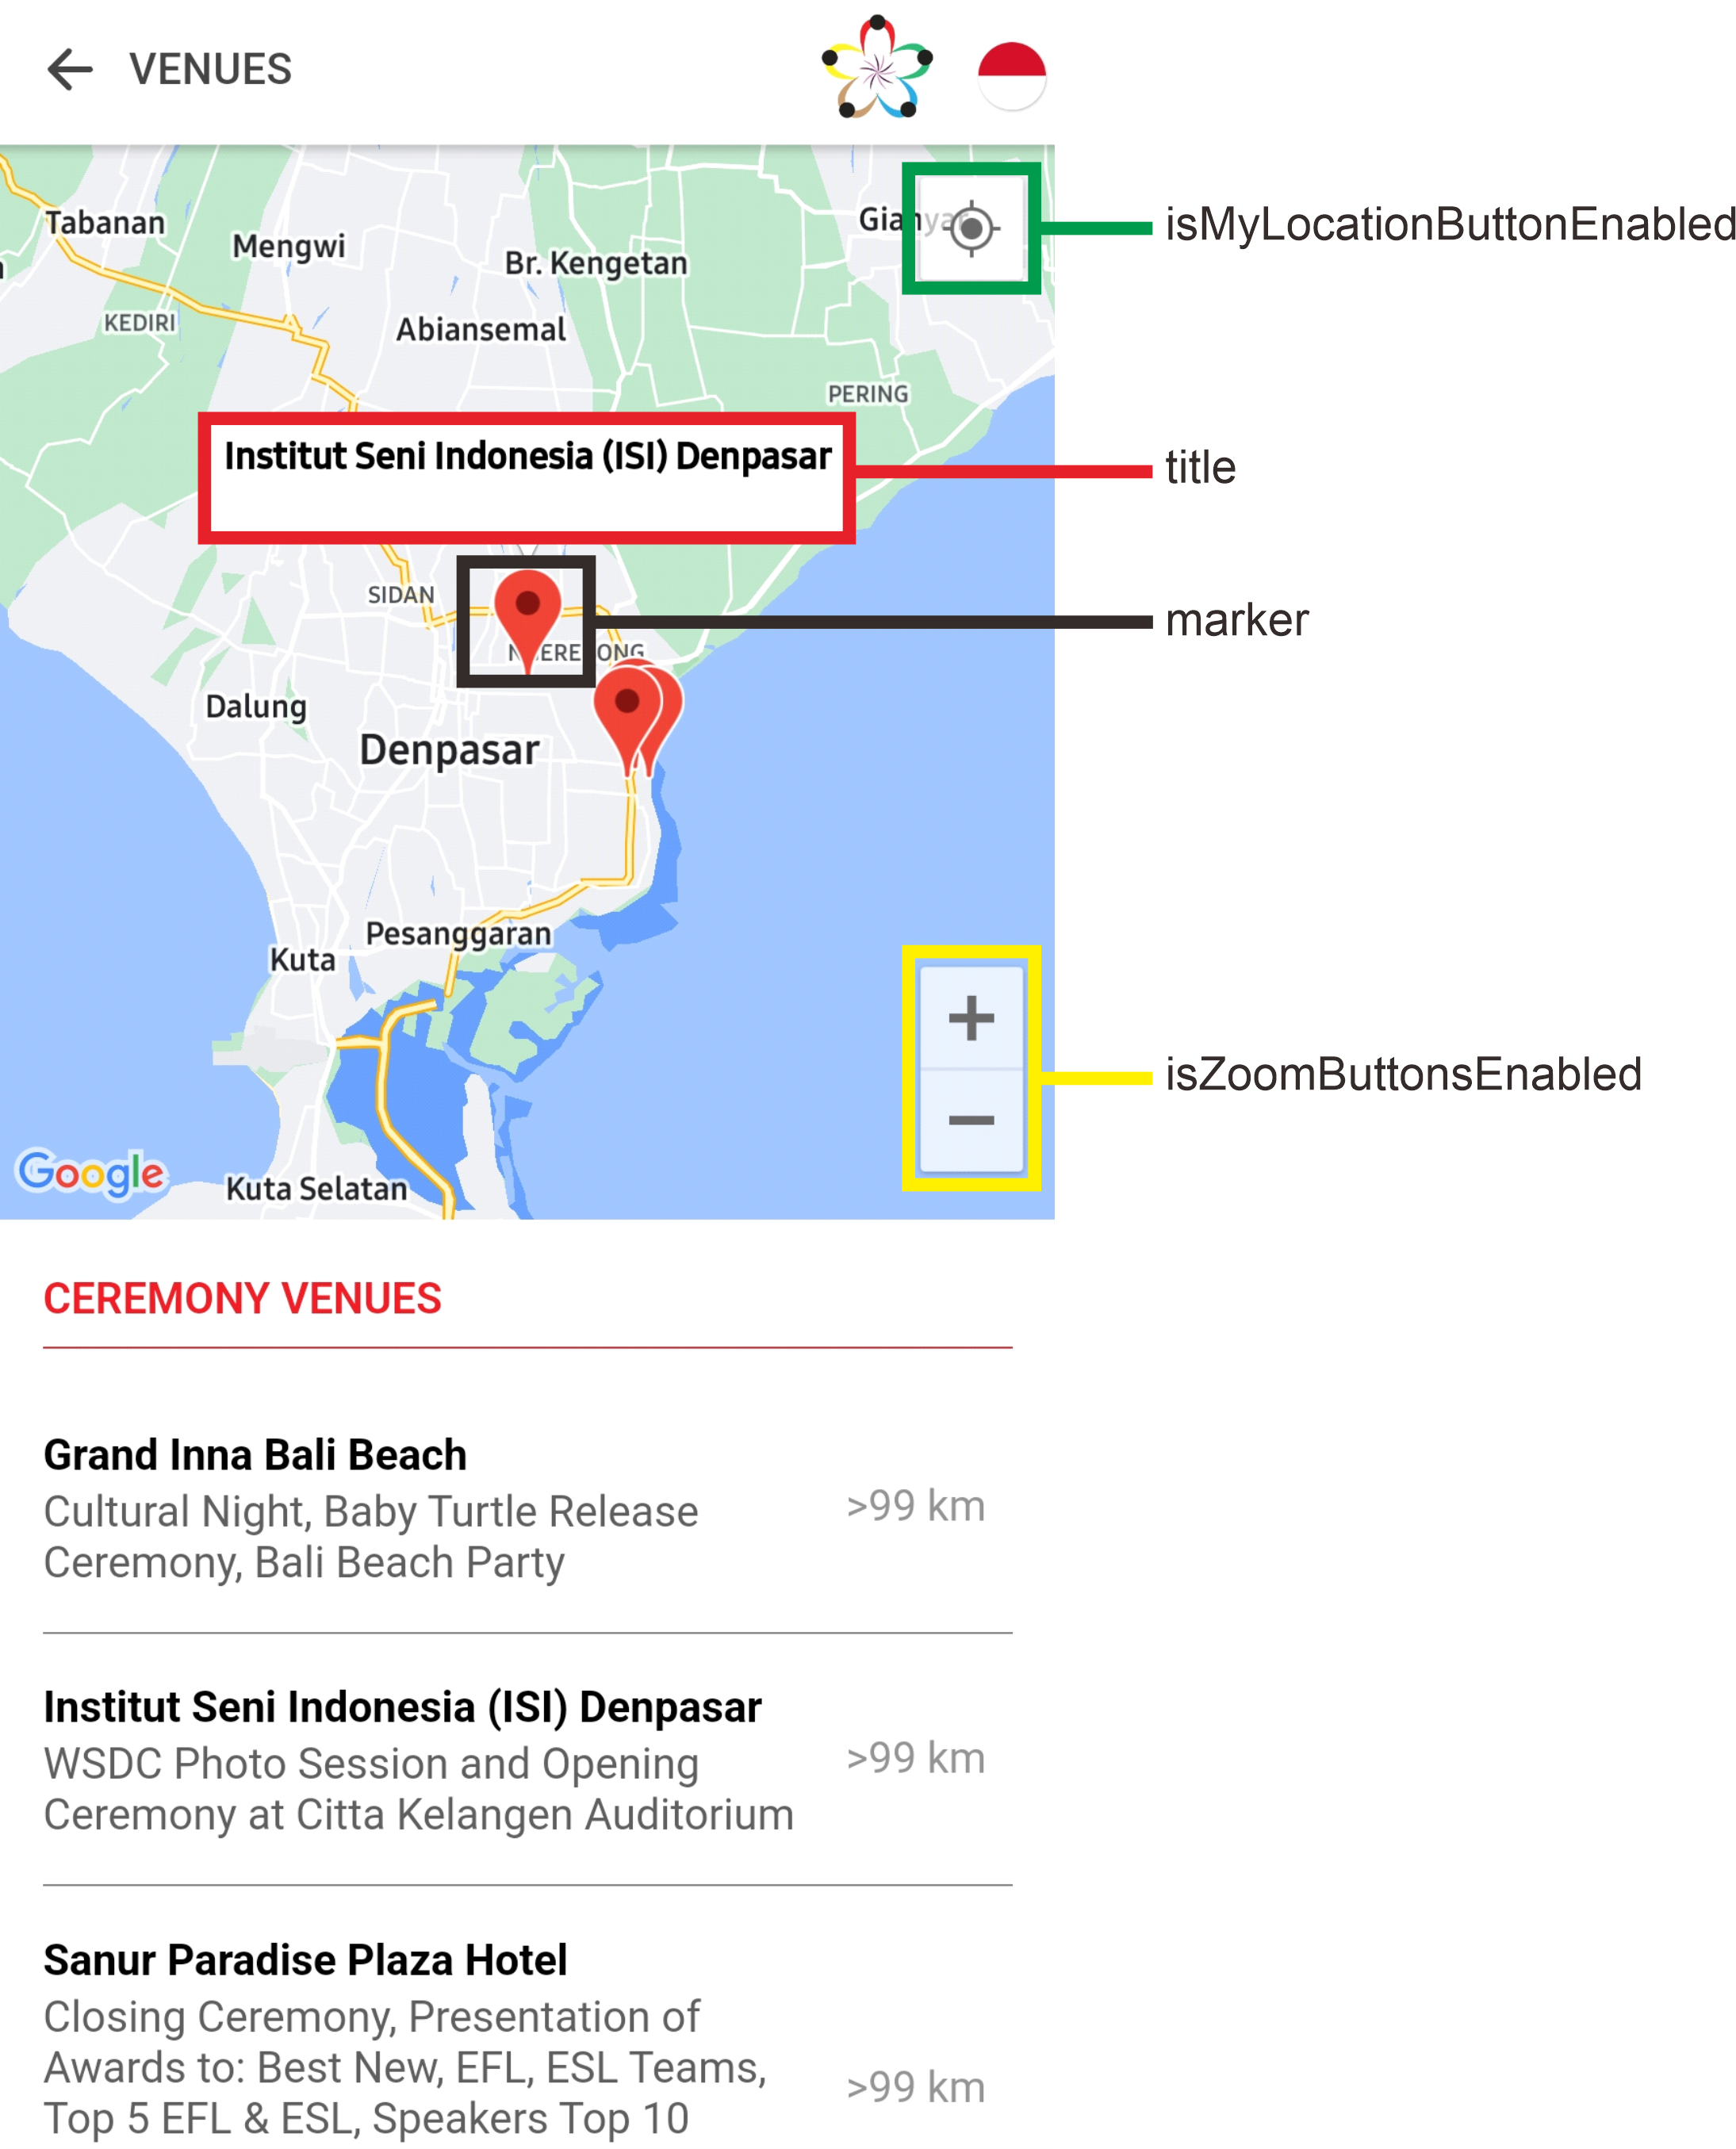
\includegraphics[width=\textwidth]{Gambar/VenueMapPageOption1.png}
         \caption{\textit{Option preferences} dan Marker}
         \label{fig:VenueMapPageOption1}
     \end{subfigure}
     \hspace*{0.5in}
     \begin{subfigure}[b]{0.45\textwidth}
         \centering
         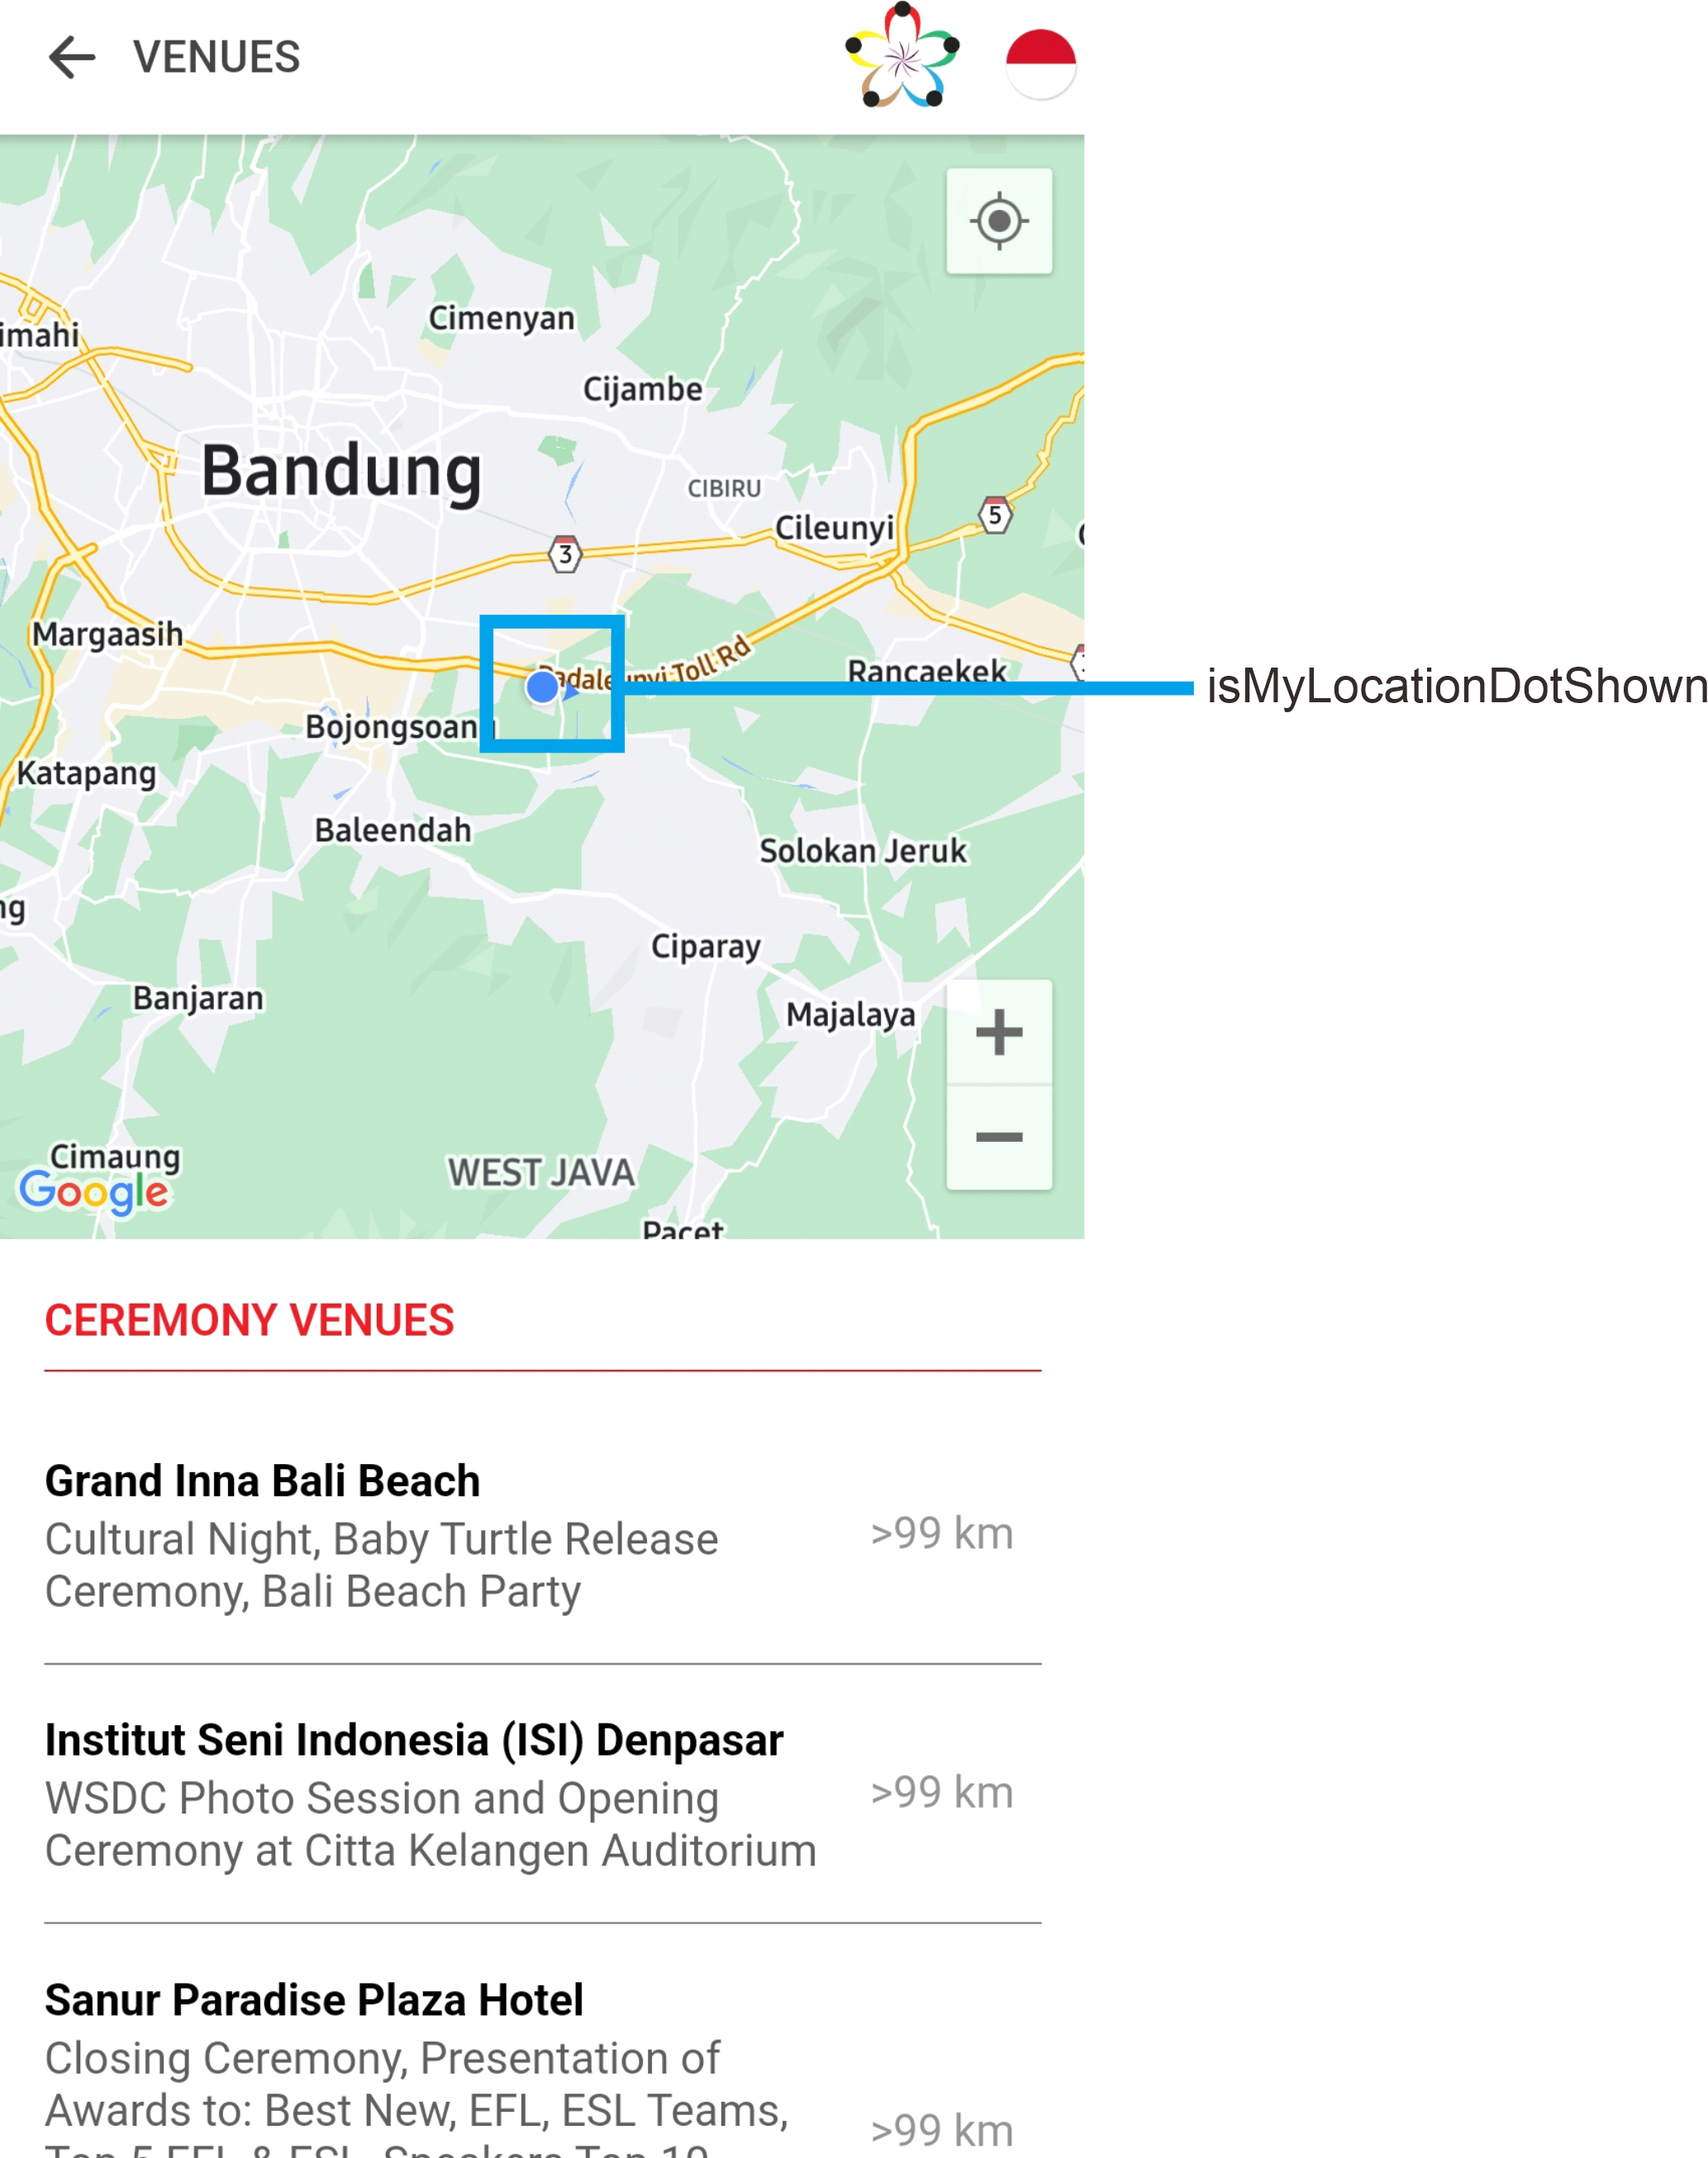
\includegraphics[width=\textwidth]{Gambar/VenueMapPageOption2.png}
         \caption{isMyLocationDotShown pada Google Maps}
         \label{fig:VenueMapPageOption2}
     \end{subfigure}
        \caption{Penggunaan Community Google Maps pada Aplikasi WSDC 2017 Bali}
        \label{fig:VenuesMapPenggunaan2}
\end{figure}
		
	\item Capacitor Geolocation API \\
	 Capacitor Geolocation API digunakan untuk mengetahui posisi dari pengguna. \textit{Plugin} ini mendapatkan koordinat berupa \textit{latitude} dan \textit{longitude} ponsel pengguna berada saat ini menggunakan \textit{Global Positioning System} (GPS) dengan menggunakan \textit{method} getCurrentPosition() seperti pada kode~\ref{lst:getposisipenggunageolocation}. Setelah mendapatkan koordinat ponsel pengguna, koordinat tersebut digunakan untuk menghitung jarak dari lokasi pengguna ke lokasi \textit{venue} seperti pada gambar~\ref{fig:jarakVenuesMap} yang ditandai dengan kotak berwarna merah. Jika lokasi pengguna dengan \textit{venue} lebih dari 99 KM dari lokasi \textit{venue}, maka akan menampilkan >99km. Jika lokasi pengguna dengan \textit{venue} kurang dari 99 KM, maka akan menampilkan jarak yang sesuai. 
\newpage
\begin{lstlisting}[label={lst:getposisipenggunageolocation}, caption=\textit{Method} getCurrentPosition( Pada Geolocation API]
const printCurrentPosition = async () => {
	const coordinates = await Geolocation.getCurrentPosition();
    this.userCoordinatesLat = coordinates.coords.latitude;
    this.userCoordinatesLng = coordinates.coords.longitude;
};
\end{lstlisting}
	 
	 \item Capacitor Splash Screen API \\
	 Capacitor Splash Screen API idigunakan untuk menampilkan \textit{splash screen} yang tampil pada saat aplikasi pertama kali dibuka. Seperti yang sudah dijelaskan pada sub-bab~\ref{subsec:capacitor}, Splash Screen secara \textit{default} otomatis ditutup setelah 500ms sejak pertama kali Splash Screen dibuka. Namun jika hal itu terjadi, maka akan ada kemungkinan ketika Splash Screen ditutup, komponen-komponen pada aplikasi belum selesai dimuat, mengakibatkan pengguna melihat halaman putih kosong. Untuk menghindari hal tersebut, Splash Screen ditutup ketika komponen Home, komponen yang pertama kali ditampilkan, selesai dimuat dan ditampilkan ke layar. Hal tersebut dapat terjadi dengan menjalankan \textit{method} hide() yang dimiliki Capacitor Splash Screen pada \textit{method} ionViewDidEnter() di dalam komponen Home seperti pada kode~\ref{lst:hidesplashscreenhome}. \textit{Method} ionViewDidEnter() sendiri merupakan sebuah Ionic Life Cycle yang dijalankan ketika komponen selesai dijalankan dan sudah ditampilkan ke layar. 
	 
\begin{lstlisting}[label={lst:hidesplashscreenhome}, caption=\textit{Method} hide() Pada Splash Screen API]
ionViewDidEnter(){
	SplashScreen.hide()
}
\end{lstlisting}

\end{itemize}

Pada sistem usulan, digunakan \textit{libraries} yang dimiliki Angular, yaitu Angular Routing dan Angular HTTPClient. Angular Routing digunakan untuk menangani navigasi dari satu tampilan ke tampilan lain, kemudian menampilkannya di layar.  Angular HTTPClient digunakan untuk melakukan komunikasi dengan server dengan menggunakan protokol HTTP. HTTPClient mendapatkan data dari server, kemudian menyimpannya ke dalam penyimpanan. HTTPClient digunakan pada setiap komponen untuk mendapatkan data dari penyimpanan. Pada komponen Home dan Announcements digunakan juga untuk mengambil data dari server seperti pada kode~\ref{lst:httpclienthome} yang merupakan penggunaan HTTPClient pada komponen Home untuk sistem kini. Pertama, Ionic Storage mengambil data terlebih dahulu dari penyimpanan. Jika aplikasi pertama kali dijalankan setelah instalasi, maka data tersebut tidak akan ada di dalam penyimpanan. Jika data tidak ada data pada penyimpanan, HTTPClient mengambil data dari aset lokal dengan \textit{method get}(), dan menyimpannya ke dalam penyimpanan dengan Ionic Storage. Jika data tidak berhasil didapatkan, maka akan menampilkan sebuah Toast. Kemudian \textit{method get}() dijalankan untuk mengambil data terbaru dari server. Data terbaru tersebut kemudian menggantikan data sebelumnya yang didapat dari lokal aset. Mengambil data pertama kali dari aset lokal bertujuan agar jika pengguna tidak terhubung ke koneksi internet pada saat pengguna melakukan instalasi aplikasi, aplikasi tetap dapat dibuka, dijalankan, dan menampilkan data-data yang seharusnya ditampilkan. Pengguna tetap mendapatkan data terbaru dari server ketika pengguna terhubung ke koneksi internet, karena \textit{method get} pada HTTPClient selalu dijalankan pada saat pengguna membuka aplikasi untuk selalu mendapatkan data terbaru dari server.
\newpage
\begin{lstlisting}[label={lst:httpclienthome}, caption=HTTPClient pada Komponen Home]
this.storage.get('wsdcDataStorage').then((data) => {
	if(data == null){
		this.http.get('../assets/json/wsdc_data.json').subscribe((data: any) => {
    		this.wsdcData = data;
        	this.storage.set('wsdcDataStorage',data);       
        },
        error => {
         	this.showToast('Failed to refresh information from local storage');
        });
	}else{    
		this.wsdcData = data;
    }
    setTimeout(() => {
        this.http.get('https://wsdc.dnartworks.com/wsdc_data.json')
        .subscribe((data: any) => {
        	this.storage.set('wsdcDataStorage', data);
          	this.wsdcData = data;
        },
        error => {
          	this.showToast('Failed to refresh information');
        });
   }, 1000);
})
\end{lstlisting} 

Perubahan-perubahan yang terjadi dan dilakukan oleh penulis dari aplikasi WSDC 2017 Bali terdahulu ke aplikasi WSDC 2017 Bali terbaru meliputi perubahan UI Component, Native API dan penggunaan \textit{plugin} dari Native API yaitu seperti pada tabel~\ref{table:perubahan}. Selain hal-hal yang berkaitan dengan perubahan-perubahan tersebut, pembuatan aplikasi WSDC 2017 Bali dengan Ionic 6 menggunakan aset yang sama dengan aplikasi WSDC 2017 Bali terdahulu, seperti gambar, file HTML, kelas TypeScript, file SCSS untuk setiap komponen, dan kode warna.

\begin{table}[H]
\centering
\caption{Tabel Perubahan yang Dilakukan dari Ionic 3 ke Ionic 6}
\begin{tabular}{|l|ll|}
\hline
\multicolumn{1}{|c|}{\multirow{2}{*}{Jenis Perubahan}} & \multicolumn{2}{c|}{Perubahan}                                                                                                               \\ \cline{2-3} 
\multicolumn{1}{|c|}{}                                 & \multicolumn{1}{l|}{Ionic 3}                                     & Ionic 6                                                                   \\ \hline
\multirow{5}{*}{UI Component}                          & \multicolumn{1}{l|}{\textless{}ion-item\textgreater{}}           & Menambahkan  \textless{}ion-label\textgreater{}                           \\ \cline{2-3} 
                                                       & \multicolumn{1}{l|}{\textless{}ion-list-header\textgreater{}}    & Menambahkan \textless{}ion-label\textgreater{}                            \\ \cline{2-3} 
                                                       & \multicolumn{1}{l|}{\textless{}button\textgreater{}}             & \textless{}ion-button\textgreater{}                                       \\ \cline{2-3} 
                                                       & \multicolumn{1}{l|}{\textless{}ion-segment-button\textgreater{}} & Menambahkan \textless{}ion-label\textgreater{}                            \\ \cline{2-3} 
                                                       & \multicolumn{1}{l|}{\textless{}ion-scroll\textgreater{}}         & Dihapus, hanya menggunakan \textless{}ion-content\textgreater sudah cukup \\ \hline
Native API                                             & \multicolumn{1}{l|}{Cordova}                                     & Capacitor                                                                 \\ \hline
\multirow{4}{*}{Plugin Native API}                     & \multicolumn{1}{l|}{Cordova Google Maps API}                     & Capacitor Community Google Maps API                                       \\ \cline{2-3} 
                                                       & \multicolumn{1}{l|}{Cordova Geolocation}                         & Capacitor Geolocation API                                                 \\ \cline{2-3} 
                                                       & \multicolumn{1}{l|}{Cordova Splash Screen}                       & Capacitor Splash Screen API                                               \\ \cline{2-3} 
                                                       & \multicolumn{1}{l|}{Cordova In-App Browser}                      & Capacitor Browser API                                                     \\ \hline
\end{tabular}
\label{table:perubahan}
\end{table}

\section{Tantangan Pengembangan Sistem Usulan}
\label{sec:analisisPermasalahanSistemKini}
Saat sedang melakukan proses migrasi aplikasi WSDC 2017 Bali dari Ionic Framework versi 3 ke Ionic Framework versi 6, terdapat beberapa kendala yang dialami. Kendala-kendala tersebut adalah sebagai berikut : 

\begin{itemize}
	\item Seperti yang disebutkan pada landasan teori (Sub Bab~\ref{subsec:migrasi}) sebelum melakukan migrasi dari Ionic Framework versi 3 ke Ionic Framework versi 6 terlebih dahulu melakukan migrasi dari Ionic Framework versi 3 ke Ionic Framework versi 4, yang selanjutnya dari Ionic versi 4 ke Ionic versi 5 dan dari Ionic versi 5 ke Ionic versi 6. Namun karena tidak tersedianya perintah untuk membuat aplikasi dengan menggunakan Ionic Framework versi 4 dan 5, maka penulis langsung melakukan migrasi dari Ionic Framework versi 3 ke Ionic Framework versi 6. Dalam melakukan hal ini, penulis berlandaskan bahwa susunan kelas Ionic Framework versi 4, 5 dan 6 tidaklah berubah sama sekali. Yang mengalami perubahan hanyalah pembaruan properti mengenai API, CSS, dan {\it package dependencies} yang terpasang, yang telah dijelaskan pada landasan teori (Sub Bab~\ref{subsec:migrasi}).
	
	\item Pada awal pengerjaan skripsi, halaman Draw dan Result pada aplikasi WSDC 2017 Bali tidak dapat diakses karena terjadi kesalahan konfigurasi pada server. Kemudian setelah menghubungi dan dibantu oleh pembuat dari aplikasi WSDC 2017 Bali, maka masalah ini telah terselesaikan, yaitu halaman Draw dan Result pada aplikasi WSDC 2017 Bali dapat diakses kembali sebagaimana mestinya.
	
	\item Pada saat pengerjaan skripsi ini, pada Desember 2021 Ionic meluncurkan generasi terbaru dari Ionic Framework, yaitu Ionic versi 6. Sedangkan Ionic versi 5 pengembangannya berhenti didukung pada tanggal 8 Juni 2022~\footnote{Status pemeliharaan dan dukungan dari setiap versi Ionic dilihat pada \url{https://ionicframework.com/docs/reference/support}}. Maka dari itu, atas saran dan masukan dosen pembimbing dan dosen penguji, maka peneliti melakukan migrasi tidak lagi sampai Ionic versi 5, melainkan sampai dengan Ionic versi 6 untuk masa dukungan Ionic Framework yang lebih lama.
	
	\item Pada Capacitor Community Google Maps, terdapat \textit{option} preferences isCompassButtonEnabled yang digunakan untuk menampilkan tombol kompas pada peta. Namun setelah aplikasi dijalankan, tombol tersebut tidak muncul pada layar. Maka hal ini menyebabkan adanya perbedaan tampilan pada peta antara aplikasi WSDC 2017 Bali terdahulu dan terbaru, yaitu tidak ada tombol kompas pada aplikasi WSDC 2017 Bali terbaru.
	
\end{itemize}